\documentclass[twocolumn]{article}

%% Language and font encodings
\usepackage[english]{babel} \usepackage[utf8x]{inputenc}
\usepackage[T1]{fontenc} \usepackage{authblk}

%% Sets page size and margins
\usepackage[a4paper,top=3cm,bottom=2cm,left=2cm,right=2cm,marginparwidth=1.5cm]{geometry}

%% Useful packages
\usepackage{amsmath}
\usepackage{graphicx}
\usepackage[colorinlistoftodos]{todonotes} \usepackage[colorlinks=true,
allcolors=blue]{hyperref}

% For algorithms
\usepackage{algorithm}
\usepackage{algorithmic}

\DeclareMathOperator*{\E}{\mathbb{E}}
\DeclareMathOperator*{\argmin}{\text{argmin}}

\usepackage[normalem]{ulem}
%\usepackage[switch]{lineno} \linenumbers
\usepackage{amsmath,amsfonts,amssymb}  % blackboard math symbols
\usepackage{bm}
\usepackage{color}
\usepackage{fancyhdr}
\usepackage{cite}
\usepackage{caption}
%\pagestyle{fancyplain}
\usepackage{tabularx}
\newcolumntype{b}{X}
\newcolumntype{s}{>{\hsize=1.09\hsize}X}
\newcolumntype{g}{>{\hsize=1.09\hsize}X}
\newcolumntype{Y}{>{\centering\arraybackslash}X}

\usepackage{etoolbox}
\appto\appendix{\addtocontents{toc}{\protect\setcounter{tocdepth}{0}}}


\DeclareMathAlphabet{\mathbbmsl}{U}{bbm}{m}{sl}
\newcommand\PP{\mathbb{P}}
\newcommand\EE{\mathbb{E}}

\newcommand{\bomu}{\ensuremath{\boldsymbol{\mu}}}
\newcommand{\boC}{\ensuremath{{\sf{C}}}}
\newcommand{\boSo}{\ensuremath{{\boldsymbol{S}_{\mathrm{o}}}}}

\numberwithin{equation}{section}

\title{\textbf{Teaching a machine to generate an artificial universe}}
\author[1]{Jed Homer\thanks{}}
\author[1]{Christopher Messenger}
\author[1]{Martin Hendry}
\affil[1]{Institute for Gravitational Research, 
          School of Physics and Astronomy, 
          University of Glasgow, G12 8QQ, UK}

%%%%%%%%%%%%%%%%%%%%%%%%%%%%%%%%%%%%%%%%%%%%%%%%%%%%%%%%%%%%%%%%%%%%%%%%%%%%%%%%%%%%%%%%%%%%%%%%%%%%%%%%%%%%%%%%%%%%%%%%%%%
%%%%%%%%%%%%%%%%%%%%%%%%%%%%%%%%%%%%%%%%%%%%%%%%%%%%%%%%%%%%%%%%%%%%%%%%%%%%%%%%%%%%%%%%%%%%%%%%%%%%%%%%%%%%%%%%%%%%%%%%%%%
%%%%%%%%%%%%%%%%%%%%%%%%%%%%%%%%%%%%%%%%%%%%%%%%%%%%%%%%%%%%%%%%%%%%%%%%%%%%%%%%%%%%%%%%%%%%%%%%%%%%%%%%%%%%%%%%%%%%%%%%%%%

\begin{document}
\date{}
%\lhead{\textbf{Version $2.7$}}

\twocolumn[
	\begin{@twocolumnfalse}
		\maketitle
		\begin{abstract}
		    This work presents a three-dimensional generative framework that uses an Auxiliary Classifier Generative
		    Adversarial Network to create realistic samples of cosmological structure at various values of redshift~$z$. 
		    Provisional samples of the virtual cosmic web are obtained from N-body simulation data that is restricted to 
		    volumes of size $200 \, h^{-1} \, \text{Mpc}$. The generated samples are shown to demonstrate
		    a high degree of coherence with their simulated counterparts and the distinction is difficult to make visually
		    by human experts. The nature of the separation between generated and N-body simulation samples is quantified 
		    with repeated tests of the Kullback-Leibler divergence on ensembles of samples alongside samples with 
		    uniformly distributed pixel densities. It is found that the implementations secure a coherence to within the
		    same order of magnitude as a self comparison of the simulation samples. The main advantage of the generative
		    approach to simulating large volumes of cosmological structure is that much less time is required than 
		    creating N-body simulations on high performance computing resources. This is demonstrated by the creation of
		    large box volumes made with $\sim10^3$ generated samples for a redshift $z$ arranged on a cubic mesh. At this 
		    stage, the generative artificial intelligence can then be said to be capable of generating an artificial 
		    universe. Future explorations of the method that are relevant to the next paradigm in cosmological simulations 
		    are also outlined. 
		  %  The most pertinent application being for a generator that can produce samples that maintain high statistical 
		  %coherence to simulation data at various redshifts. 
            %\textit{}
		\end{abstract}
	\end{@twocolumnfalse}
]
{\renewcommand{\thefootnote}%
    {\fnsymbol{footnote}}
  \footnotetext[1]{Corresponding author: \url{jedhmr@gmail.com}}
}

% \setcounter{tocdepth}{2}
% \begingroup
% \let\clearpage\relax
% \tableofcontents
% \endgroup
% \newpage

%%%%%%%%%%%%%%%%%%%%%%%%%%%%%%%%%%%%%%%%%%%%%%%%%%%%%%%%%%%%%%%%%%%%%%%%%%%%%%%%%%%%%%%%%%%%%%%%%%%%%%%%%%%%%%%%%%%%%%%%%%%
%%%%%%%%%%%%%%%%%%%%%%%%%%%%%%%%%%%%%%%%%%%%%%%%%%%%%%%%%%%%%%%%%%%%%%%%%%%%%%%%%%%%%%%%%%%%%%%%%%%%%%%%%%%%%%%%%%%%%%%%%%%
%%%%%%%%%%%%%%%%%%%%%%%%%%%%%%%%%%%%%%%%%%%%%%%%%%%%%%%%%%%%%%%%%%%%%%%%%%%%%%%%%%%%%%%%%%%%%%%%%%%%%%%%%%%%%%%%%%%%%%%%%%%

\section{Introduction}
Beyond the distance scales of galactic diameters, toward the sizes of galaxy clusters and beyond, matter in the Universe 
appears as a webbed structure of filaments across volumes of emptiness known as voids. This network of luminous formation 
is known as the cosmic web~\cite{bond_cw1, Coles_cw2, Forero_cw3, Dietrich_cw4, cw_phenomenon}. The cosmic web as a 
distribution of matter contains artefacts linked to the state of the primordial universe, the nature of early universe 
perturbations and more fundamental physics to describe this era in cosmic time. The emergence of the structure is from 
an early period of exponential expansion, known as inflation~\cite{inflation_cosmo2}. This structure has been observed by 
missions such as~\cite{sdss1, 2df} and by weak gravitational lensing~\cite{glens_book} through distortions, or 
shears~\cite{shear_review}, to images of distant galaxies caused by the large-scale structure of the universe. 

The webbed structure is native to the well-established $\Lambda$ Cold Dark Matter ($\Lambda \text{CDM}$) cosmology but 
its exact origins are not well understood~\cite{class_perturbs} and at present it is believed that the structure originates 
from an amplification of quantum fluctuations as a density perturbation in the early universe~\cite{perturbation_theory}, 
which is described by inflationary cosmology~\cite{inflation_cosmology}. The matter distribution of webbed structure in 
the universe holds information on the true nature of dark matter, dark energy, the laws of gravity and the mode of galaxy 
formation~\cite{DarkEnergySurvey, kids_lensing, kids_cosmo, gal_formation, gal_formation2}.

% PROBLEMS, FUTURE HOPES, SIMULATIONS
Simulations that trace the evolution of phenomena such as structure formation, galaxy populations and the distribution of 
matter are imperative to our understandings of cosmological measurements. Our insight into the high-redshift deep field 
will increase with the amount of information provided by next generation observational missions such 
as~\cite{wfirst_afta, euclid, LSST}. As a consequence, so too does the need for higher resolution and more capacity in 
the volumes of simulated universes. Evidence for new theory in cosmology can come from greater observational resolution. 
This level of detail informs research into baryonic acoustic oscillations within the matter 
distribution~\cite{bao,bao2,bao3}. Undoubtedly new information will emerge on these dilemmas in cosmology. This sets the 
next paradigm of the field in the study of smaller scales of cosmological structure.

Clearly there is a need for coherent simulations that are summarised by the same statistics as galaxy surveys such as 
the 2dF Galaxy Redshift Survey~\cite{2df}. These simulations will then contain the same environments of large scale
structure as observations to check experimental measurements with. Obtaining these more realistic 
simulations~\cite{mill2sim, millxxlsim} involves using greater computational resources and theoretical analysis. The 
latter of the two, due to the complexity of the non-linear physics that describes the growth of structure over cosmic time, 
shows some differences to observations~\cite{mill_diffs}. A resource that could effectively reproduce the statistical 
properties of observations and simulations by learning the distribution in an advanced simulation (and therefore potentially
of nature) without any assumptions of these properties would be of great value. This work aims to validate a method for 
obtaining a resource capable of achieving this objective by synthesising both 2D and 3D images from existing simulation 
data for two separate Generative Adversarial Networks (GANs) to emulate. 

% SOME EXAMPLES OF GENERATIVE AI
Deep learning has evolved to be able to process the statistical structure of the hierarchy of features in the visual 
domain~\cite{nvidia_gan}. There have been a number of recent applications of generative deep learning in astrophysics. 
GANs have been used to create new samples of galaxy images~\cite{gal_im_gen2} and to obtain visual characteristics past
the deconvolution limit~\cite{gal_im_gen3}. Other applications use the GAN framework to generate 2D images of the cosmic 
web~\cite{web_gan} and projected 2D mass distributions, known as convergence maps, from simulated data of weak 
gravitational lensing within the environment of an N-body simulation~\cite{cosmogan}. This report will show the insights 
that the study of astrophysics can have on AI through applications of statistics that could give new mechanisms for
maximizing the realism of GAN generated samples. 

This work is organised as follows. Section~\ref{sec:ai_intro} will introduce the domain in which the methods for 
generating new galaxy-distribution samples originate. This section will introduce the sub-field of generative artificial 
intelligence and its relevance to the experimental method. Section~\ref{sec:gans} will describe Generative Adversarial 
Networks (GANs), their analytical properties and how these models learn to imitate datasets. Section~\ref{sec:related_work} 
will study the present state of the concepts from the previous sections with respect to recent research in physics and 
astrophysics. Section~\ref{sec:universe_applications} discusses some of the applications for successful potential of the 
work, that is, being able to generate distributions of galaxies that are coherent with N-body simulation data. 
Section~\ref{sec:methods} describes the methods of extracting and pre-processing training data from N-body simulations, 
the setup of each training loop for the GAN implementations and the architectures of the generative models. 
Section~\ref{sec:stats_and_diags} gives insight into the methods of comparison between the generated and training 
distributions and finally Sections~\ref{sec:results},~\ref{sec:future_work} and~\ref{sec:conclusions} present the results, 
future work and conclusions.

%%%%%%%%%%%%%%%%%%%%%%%%%%%%%%%%%%%%%%%%%%%%%%%%%%%%%%%%%%%%%%%%%%%%%%%%%%%%%%%%%%%%%%%%%%%%%%%%%%%%%%%%%%%%%%%%%%%%%%%%%%%
%%%%%%%%%%%%%%%%%%%%%%%%%%%%%%%%%%%%%%%%%%%%%%%%%%%%%%%%%%%%%%%%%%%%%%%%%%%%%%%%%%%%%%%%%%%%%%%%%%%%%%%%%%%%%%%%%%%%%%%%%%%
%%%%%%%%%%%%%%%%%%%%%%%%%%%%%%%%%%%%%%%%%%%%%%%%%%%%%%%%%%%%%%%%%%%%%%%%%%%%%%%%%%%%%%%%%%%%%%%%%%%%%%%%%%%%%%%%%%%%%%%%%%%

\begin{figure}
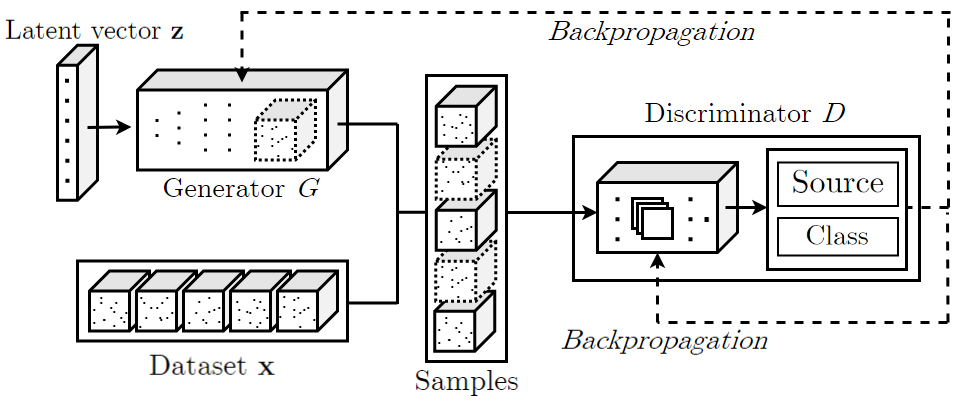
\includegraphics[width=\columnwidth, trim=4 4 4 4,clip]{figures/diagrams/ACGAN_diagram_box.png}
\centering
\caption{Schematic of the GAN framework; including discriminator and generator networks, the latent-space vector, dataset 
         of samples and the backpropagation feedback to model parameters. \textit{Source} and \textit{Class} refer to the
         values of $p_\mathbf{x}$ and $p_\mathbf{c}$ designated by the discriminator on a sample $\mathbf{x}$.}
\label{fig:GAN_diagram}
\end{figure}


\begin{figure*}%[hbt!]
\includegraphics[width=15cm]{figures/diagrams/gan_game.png}
\centering
\caption{A diagram of the simplified two-parameter value function $V$ for the zero-sum game in which the generator $G$ and 
discriminator $D$ participate in; (a) - the value function in parameter space with a Nash equilibrium point, (b) - The 
maximization objective for $G$ with $\theta^{(D)}=0$ and (c) - the minimization task for $D$ with $\theta^{(G)}=0$.}
\label{fig:gan_game}
\end{figure*}

%%%%%%%%%%%%%%%%%%%%%%%%%%%%%%%%%%%%%%%%%%%%%%%%%%%%%%%%%%%%%%%%%%%%%%%%%%%%%%%%%%%%%%%%%%%%%%%%%%%%%%%%%%%%%%%%%%%%%%%%%%%
%%%%%%%%%%%%%%%%%%%%%%%%%%%%%%%%%%%%%%%%%%%%%%%%%%%%%%%%%%%%%%%%%%%%%%%%%%%%%%%%%%%%%%%%%%%%%%%%%%%%%%%%%%%%%%%%%%%%%%%%%%%
%%%%%%%%%%%%%%%%%%%%%%%%%%%%%%%%%%%%%%%%%%%%%%%%%%%%%%%%%%%%%%%%%%%%%%%%%%%%%%%%%%%%%%%%%%%%%%%%%%%%%%%%%%%%%%%%%%%%%%%%%%%

\section{Generative Adversarial Networks}\label{sec:gans}
% what are GANs, what do D and G do, how do D and G work, how does this change over training,
% GANS ARE GOOD, EXAMPLES OF GANS

The type of generative model chosen for the objective of this work was the Auxiliary Classifier Generative Adversarial 
Network (ACGAN) created by Odena et al. 2017~\cite{acgan} which is an extension to the original GAN invented by Goodfellow 
et al. 2014~\cite{gf_gan}. The successes of GANs are well established in a wide range of applications on natural 
images~\cite{wgan, karrasgan, largegan} and there are many extensions to GANs that open up a wide range of other successful models~\cite{pix2pix, hiresgan, lapgan}. 

% BASICS: WHAT DO D AND G DO?
Generative Adversarial Networks consist of two models known as the generator and the discriminator. The generator must 
create samples that are allegedly drawn from the same distribution as the real samples dataset. The discriminator assigns 
scalars to a collection of input data and generated samples, each representing the probability that a sample is either real 
and from the data distribution $p_{data}$ or fake and from the model distribution  $p_{model}$. The discriminator has 
access to both real and fake samples. The training of a GAN involves navigating the combined parameter space of the 
generator and discriminator network parameters to find the optimal value of a function that gives the best performance of
the networks at their opposing objectives. The metric that describes the performance is related to the distance between 
the model and data distributions. There is no need for a validation subset external to the training data because the 
generator does not have direct access to the training data. This is not the case for singular deep learning networks.

%%%%%%%%%%%%%%%%%%%%%%%%%%%%%%%%%%%%%%%%%%%%%%%%%%%%%%%%%%%%%%%%%%%%%%%%%%%%%%%%%%%%%%%%%%%%%%%%%%%%%%%%%%%%%%%%%%%%%%%%%%%
%%%%%%%%%%%%%%%%%%%%%%%%%%%%%%%%%%%%%%%%%%%%%%%%%%%%%%%%%%%%%%%%%%%%%%%%%%%%%%%%%%%%%%%%%%%%%%%%%%%%%%%%%%%%%%%%%%%%%%%%%%%

\subsection{Generative adversarial learning}
% introduce adversarial relation / game between D and G
The discriminator and the generator are neural networks that each network try to reduce their own objective function. 
This adversarial relationship is a game between the models rather than two optimisation problems. The optimum in this 
case is a Nash equilibrium~\cite{NIPS16} rather than a local minimum given by optimisation in the case of a singular 
neural network. In this equilibrium the returns of the objective functions only change by indirect influence of the 
other network and at this stage the gradients for backpropagation to either model have vanished.

% WHAT ARE D AND G? HOW DO D AND G WORK?
% The discriminator and generator models can be represented as functions $D$ and $G$ respectively because of their 
% mappings as neural networks and parameter dependencies. 
The discriminator $D$ has image input $\mathbf{x}$ and parameters 
$\bm{\theta}^{(D)}$. The generator $G$ takes a latent space vector $\mathbf{z}$ as input and uses parameters 
$\bm{\theta}^{(G)}$. 
% Information flows through the network and its parameters to create the outputs $D(\mathbf{x})$ or 
% $D(G(\mathbf{z}))$ for the discriminator and $G(\mathbf{z})$ for the generator. This is the forward-propagation from 
% an input to an output. The model performances are calculated with the objective functions $J^{(D)}$ or $J^{(G)}$. 

% HOW DO D AND G WORK TOGETHER IN A GAN AND PLAY THE GAME?
In the case of a GAN, the optimisation landscape is more complex because of the simultaneous learning of the two 
neural networks that both constantly adjust their parameters. 
% The discriminator and generator models in a GAN depend on parameters $\bm{\theta}^{(D)}$ and $\bm{\theta}^{(G)}$ respectively. 
% The models typically consist of multi-layer 
% perceptrons with the potential for other parametric components such as convolutional layers and the parameters are 
% the state of these components at an epoch of training. 
The generator $G$ draws noise vectors $\mathbf{z}$ from a prior 
distribution $p_{\mathbf{z}}$. The vectors $\mathbf{z}$ are passed through the generator architecture to create a 
sample $\mathbf{x}=G(\mathbf{z};\bm{\theta}^{(G)})$ that is now a sample $\mathbf{x}$ from the model distribution 
$p_{model}$ - this is the distribution of generated samples $G(\mathbf{z})$ obtained from passing 
latent vectors $\mathbf{z}$ through $G$ such that $\mathbf{z} \sim p_{\mathbf{z}}$. The learning of the generator 
means that the samples evolve over the training process. Eventually, the samples will appear to have been drawn 
from the true data distribution $p_{data}$ so that $G(\mathbf{z}) \sim p_{data}$. The generated samples 
$\mathbf{x} \sim p_{model}$ and real samples $\mathbf{x} \sim p_{data}$ become indistinguishable. 

The mapping learnt by the generator is expressed as $G \! : \! \mathbf{z} \! \mapsto \! \mathbf{x}$. The 
discriminator $D$ is a map from an input of real $\mathbf{x}$ and fake samples $G(\mathbf{z})$ to an output of 
as many probabilities. The values of  $D(\mathbf{x})$ and $D(G(\mathbf{z}))$ signify the discriminator's confidence 
in the validity of the sample. This mapping is expressed as $D \! : \! \mathbf{x} \!  \mapsto \! [0,1]$. 

%%%%%%%%%%%%%%%%%%%%%%%%%%%%%%%%%%%%%%%%%%%%%%%%%%%%%%%%%%%%%%%%%%%%%%%%%%%%%%%%%%%%%%%%%%%%%%%%%%%%%%%%%%%%%%%%%%%%%%%%%%%
%%%%%%%%%%%%%%%%%%%%%%%%%%%%%%%%%%%%%%%%%%%%%%%%%%%%%%%%%%%%%%%%%%%%%%%%%%%%%%%%%%%%%%%%%%%%%%%%%%%%%%%%%%%%%%%%%%%%%%%%%%%

\subsubsection{Formulation of GAN learning}
% D vs G in adversarial environment, value function and game in parameter space
The objective functions of $D$ and $G$ are defined in terms of both players' parameters and are denoted by 
$J^{(D)}(\bm{\theta}^{(D)}, \bm{\theta}^{(G)})$ and $J^{(G)}(\bm{\theta}^{(D)}, \bm{\theta}^{(G)})$~respectively. 
In the most basic adversarial setting for the GAN models, $D$ and $G$ play a zero-sum game where $J^{(D)} = - J^{(G)}$.

During training the discriminator minimises $J^{(D)}$ only through feedback from backpropagation to its parameters 
$\bm{\theta}^{(D)}$. The generator $G$ minimises $J^{(G)}$ by only affecting its parameters $\bm{\theta}^{(G)}$ through 
returns from backpropagation related to the discriminator classifications. The minimization objectives are simultaneous 
between two networks in search of a Nash equilibrium and added together the objectives for the discriminator and generator 
give a value function $V(\bm{\theta}^{(D)}, \bm{\theta}^{(G)})$ in the combined parameter space $(\bm{\theta}^{(D)}, 
\bm{\theta}^{(G)})$. Figure~\ref{fig:gan_game} shows the value function in the combined parameter space for which the 
backpropagation gradients are calculated 
%with $D$ and $G$ as adversaries of each other. 
The optimum parameters for each 
network are shown at the Nash equilibrium. The game between the models is described with the value function $V$ as 

\begin{eqnarray}\label{eqn:value}
    \min_G \max_D V(D,G) &=& \mathbb{E}_{\mathbf{x}\sim p_{data}}\log D(\mathbf{x})            \nonumber \\
                         &+& \mathbb{E}_{G(\mathbf{z}) \sim p_{model}}\log(1-D(G(\mathbf{z}))) \nonumber \\
\end{eqnarray}

in the combined parameter space. The expectation operators 
$\mathbb{E}_{\mathbf{x} \sim p_{data}}$ and $\mathbb{E}_{G(\mathbf{z}) \sim p_{model}}$ correspond to the ensemble 
averages over the classifications of real and fake samples respectively. This equation shows the opposition between 
the maximization of the correct classifications by $D$ and the minimisation of the correct classifications by $D$ of 
the generator products that are made by $G$. 

The Nash equilibrium is satisfied by a pair of parameter sets $(\bm{\theta}^{(D)*}, \bm{\theta}^{(G)*})$ for which 
no further changes occur to the objective functions $J^{(D)}$ and $J^{(G)}$ of both networks~\cite{NIPS16}. 
Equation~\ref{eqn:value} means that the zero-sum game for the models returns an adjustment $+V$ for the discriminator 
and $-V$ for the generator. Figure~\ref{fig:gan_game} shows the equilibrium point in the parameter space and the 
returns $V(\bm{\theta}^{(D)}, 0)$ and $V(0, \bm{\theta}^{(G)})$ for the discriminator and generator with optimum 
parameters $\bm{\theta}^{(D)*}$ and $\bm{\theta}^{(G)*}$ respectively in the zero-sum game. The zero-sum game between 
$D$ and $G$ defines an objective function $J^{(D)}$ for the discriminator

\begin{eqnarray}\label{eq:J_D}
    J^{(D)} &=& \mathbb{E}_{\mathbf{x} \sim p_{data}}\log D(\mathbf{x})  \nonumber \\
            &+&\mathbb{E}_{G(\mathbf{z}) \sim p_{model}}\log (1 - D(G(\mathbf{z})))
\end{eqnarray}

this is from the cross-entropy discriminator objective function for the binary classification of real and fake 
samples. Appendix~\ref{appendix:cross_entropy} defines cross-entropy in this context. Equation~\ref{eq:J_D} shows that the first 
term cannot be influenced by the generator $G$ because here the samples are drawn from the data distribution to which 
it has no access to. Inputs to the generator $\mathbf{z}$ are drawn from the prior distribution $p_\mathbf{z}$ over 
the latent-space to the model. The discriminator is given a generator sample $G(\mathbf{z})$ to classify it as fake, 
so $D(G(\mathbf{z})) \! \rightarrow \! 0$ whereas the generator $G$ tries to make $D(G(\mathbf{z})) \!  \rightarrow \! 1$. 
The Nash equilibrium is satisfied for the model and data distributions becoming identical (in the ideal case) so that 
$G(\mathbf{z})$ is drawn from $p_{data}$. This means the discriminator classification tends to $D(\mathbf{x}) = 
\frac{1}{2}$ for all samples~$\mathbf{x}$~\cite{gf_gan}. The optimum of the generator $G$ parameters 
$\bm{\theta}^{(G)*}$ is 

\begin{equation}
    \bm{\theta}^{(G)*} = \argmin_{\mathbf{\theta}^{(G)}}\max_{\mathbf{\theta}^{(D)}}
                          V({\mathbf{\theta}^{(D)}},{\mathbf{\theta}^{(G)}})
\end{equation}

This motivates the generator to increase the likelihood of the discriminator incorrectly classifying a sample. The 
discriminator tries to increase its own likelihood of correctly classifying a sample by minimising the binary 
cross-entropy objective. The local minima of the value function $V$ are not necessarily Nash equilibrium points, rather
they are points that simultaneously minimise the objective functions $J^{(D)}$ and $J^{(G)}$. Whilst both networks search 
the parameter space via SGD of the value function, there is no guarantee of a Nash equilibrium, this is part of what makes 
training an adversarial model such a difficult task.

% The cross-entropy for the discriminator classification of a sample against the true label of the sample is numerically 
% effective for a GAN in practice because this objective does not saturate for an incorrect identification. Because the 
% networks try to minimize their opposing objectives, if the discriminators performance increases enough, the generator 
% objective function tends to zero. This causes the generator performance to become static. At all points in the parameter 
% space the generator objective minimization is guided by the gradients from backpropagation which will reduce to zero. At 
% this point the discriminator cannot improve and less information is back-propagated through the networks.

The solution, shown in~\cite{gf_gan}, is to deviate from the zero-sum ideal by inverting the target used to create the 
cross-entropy objective function for the generator. The generator's objective function becomes

\begin{equation}\label{eqn:J_G}
    J^{(G)} = \mathbb{E}_{G(\mathbf{z}) \sim p_{model}} \log D(G(\mathbf{z}))  
\end{equation}

Now the generator tries to maximize the log-probability of the discriminator wrongly classifying a given sample. This 
objective with the original objective for the discriminator $J^{(D)}$ means there are always non-vanishing gradients for 
backpropagation despite any imbalance in discriminator and generator performance. 

%%%%%%%%%%%%%%%%%%%%%%%%%%%%%%%%%%%%%%%%%%%%%%%%%%%%%%%%%%%%%%%%%%%%%%%%%%%%%%%%%%%%%%%%%%%%%%%%%%%%%%%%%%%%%%%%%%%%%%%%%%%
%%%%%%%%%%%%%%%%%%%%%%%%%%%%%%%%%%%%%%%%%%%%%%%%%%%%%%%%%%%%%%%%%%%%%%%%%%%%%%%%%%%%%%%%%%%%%%%%%%%%%%%%%%%%%%%%%%%%%%%%%%%

\subsubsection{Experimental design of GANs} 
The opposing players in the zero-sum game are assumed by two deep convolutional neural network (DCNN) models. These 
networks use convolutional layers to extract features from grid-like data. Deep Convolutional Generative Adversarial 
Networks (DCGANs), first implemented by Radford et al. 2015~\cite{dcgan}, use these layers to create images. The DCGAN 
model has shown excellent results on natural image generation using the CelebA~\cite{celebA} and the 
LSUN-Bedrooms~\cite{LSUN} datasets. The DCNNs in this work are based on the AlexNet models for image 
classification~\cite{dcnn}. Despite most of the architectural features, such as convolutional layers, being used in deep 
learning models prior to this publication the DCGAN architecture improved previous GAN architectures for increased 
performance in image generation tasks. The models in the methods of this work borrow from the ideas of this architectural 
basis.

%%%%%%%%%%%%%%%%%%%%%%%%%%%%%%%%%%%%%%%%%%%%%%%%%%%%%%%%%%%%%%%%%%%%%%%%%%%%%%%%%%%%%%%%%%%%%%%%%%%%%%%%%%%%%%%%%%%%%%%%%%%
%%%%%%%%%%%%%%%%%%%%%%%%%%%%%%%%%%%%%%%%%%%%%%%%%%%%%%%%%%%%%%%%%%%%%%%%%%%%%%%%%%%%%%%%%%%%%%%%%%%%%%%%%%%%%%%%%%%%%%%%%%%

\subsection{Auxiliary-Classifier GANs}
The ability to generate different classes of an object does not require separate and independent GANs. The GAN framework 
may be supplemented by an auxiliary classifier model that is attached to the discriminator model, which still classifies 
the samples as real and fake, whilst additionally characterising the pre-designated class of the object. This augmented 
GAN was derived by Odena et al. 2017 \cite{acgan} and is referred to as an Auxiliary Classifier Generative Adversarial 
Network (ACGAN). The application to this method is that the different redshift data available from N-body simulations can 
be classified and given to an ACGAN. The generator component of this model can then create samples at different redshifts. 
These samples could be tessellated together to form a larger distribution across a continuous range of  redshifts. A very 
similar method known as a Conditional-GAN (CGAN)~\cite{cgan} is known to work well at the same task.

In the ACGAN framework each sample $\mathbf{x}$ (generated or not) has a corresponding label $c_)\mathbf{x} \sim p_c$ and noise vector $\mathbf{z} \sim p_\mathbf{z}$ 
which make the generator create a sample $G(c_\mathbf{x}, \mathbf{z})$ where $G(c_\mathbf{x}, \mathbf{z}) \in X_\textup{fake}$.
The discriminator $D$ gives probability distributions $P(S|X)$ and $P(C|X) = D(X)$ over the sources of the samples $S \in \{X_\textup{real}, X_\textup{fake}\}$ and class labels $C$. The objective function is made of two independent parts; the 
likelihood of a correct source $L_S$ and the log-likelihood of the correct class $L_C$

\begin{eqnarray}
    % L_S &=& \EE [\log P(S = \textup{real} | X_{real})] \nonumber \\
    %     &+& \EE [\log P(S = \textup{fake} | X_{fake})] \\ 
    %     & & \nonumber \\ 
    % L_C &=& \EE [\log P(C = c | X_{real})] \nonumber \\
    %     &+& \EE [\log P(C = c | X_{fake})]
    L_S &=& \EE [\log P(\mathbf{x} \sim p_{\textup{data}} | \mathbf{x} \sim X_{real})] \nonumber \\
        &+& \EE [\log P(\mathbf{x} \sim p_{\textup{model}} | \mathbf{x} \sim X_{fake})] \\ 
        & & \nonumber \\ 
    L_C &=& \EE [\log P(c_\mathbf{x} = c \, | \mathbf{x} \sim X_{real})] \nonumber \\
        &+& \EE [\log P(c_\mathbf{x} = c \, | \mathbf{x} \sim X_{fake})]
\end{eqnarray}

In this case $D$ tries to maximize $L_S + L_C$ and $G$ tries to minimise $L_C - L_S$.

% Label embedding, one hot encoding, cross entropy

\begin{figure}
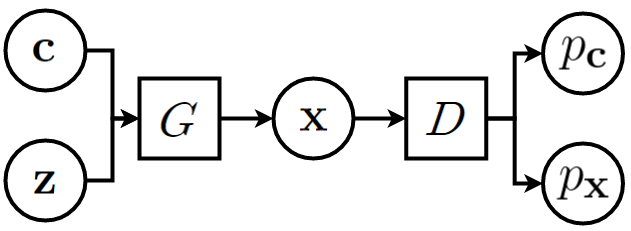
\includegraphics[width=\columnwidth]{figures/diagrams/ACGAN_diagram.png}
\centering
\caption{Schematic of the ACGAN framework; including discriminator and generator networks, the latent-space 
         vector~$\mathbf{z}$, the class label~$\mathbf{c}$, image~$\mathbf{x}$ and the discriminator 
         classifications of the class and source of an image $p_{\mathbf{x}}$ and $p_\mathbf{c}$.}
\label{fig:GAN_diagram}
\end{figure}

%%%%%%%%%%%%%%%%%%%%%%%%%%%%%%%%%%%%%%%%%%%%%%%%%%%%%%%%%%%%%%%%%%%%%%%%%%%%%%%%%%%%%%%%%%%%%%%%%%%%%%%%%%%%%%%%%%%%%%%%%%%
%%%%%%%%%%%%%%%%%%%%%%%%%%%%%%%%%%%%%%%%%%%%%%%%%%%%%%%%%%%%%%%%%%%%%%%%%%%%%%%%%%%%%%%%%%%%%%%%%%%%%%%%%%%%%%%%%%%%%%%%%%%

% \subsection{Fourier Transform ACGAN (FT-ACGAN)}
% write this if I get it to work

%%%%%%%%%%%%%%%%%%%%%%%%%%%%%%%%%%%%%%%%%%%%%%%%%%%%%%%%%%%%%%%%%%%%%%%%%%%%%%%%%%%%%%%%%%%%%%%%%%%%%%%%%%%%%%%%%%%%%%%%%%%
%%%%%%%%%%%%%%%%%%%%%%%%%%%%%%%%%%%%%%%%%%%%%%%%%%%%%%%%%%%%%%%%%%%%%%%%%%%%%%%%%%%%%%%%%%%%%%%%%%%%%%%%%%%%%%%%%%%%%%%%%%%
%%%%%%%%%%%%%%%%%%%%%%%%%%%%%%%%%%%%%%%%%%%%%%%%%%%%%%%%%%%%%%%%%%%%%%%%%%%%%%%%%%%%%%%%%%%%%%%%%%%%%%%%%%%%%%%%%%%%%%%%%%%

\section{Related work}\label{sec:related_work}
Over the last few years research has accumulated on the different applications of GANs to emulating data samples. An 
example of GANs being able to provide new data for further statistical insight is in the domain of particle physics. Here, 
GANs have been used to generate particle beams~\cite{muon_beams_gan}, particle interaction-showers~\cite{particle_showers_gan} 
and 2D images of jets~\cite{particle_jets_gan}. The DCGAN architecture has consistently shown that it could generalise well 
in astrophysical applications. The ability for GANs to transfer to new data and generalise to different types of data has 
been founded by many publications with a variety of target data.

Aside from the research into GANs for image based tasks, less work exists that uses generative AI in astrophysics. One 
application of GANs to astrophysical data concerns subverting the point spread function (PSF) that describes the effect 
of noise on the clarity of images~\cite{gal_im_gen3}. Typically the deconvolution of the separate noise and true light 
distributions are limited by the Nyquist sampling effect. The findings indicate the GAN approach successfully obtains 
artefacts within images that have low signal-to-noise ratios. See~\cite{gal_im_gen2} for a similar example of research 
using GANs in generating astronomical images.

Rodriguez et al. 2018~\cite{web_gan} use GANs to generate realistic 2D samples of N-body simulation mass distributions 
of size $100 \: h^{-1} \,\textup{Mpc}$ and $500 \: h^{-1} \,\textup{Mpc}$. This paper is the closest to the work 
presented in this report. N-body simulation data was obtained from the particle distribution of the L-PICOLA 
simulation~\cite{LPICOLA} at $z=0$. This simulation is based on the $\Lambda \text{CDM}$ cosmological model with 
the Hubble constant $H_0=70\textup{ km s}^{-1}\textup{ Mpc}^{-1}$, dark energy density $\Omega_\Lambda=0.72$ and
matter density $\Omega_m=0.28$. The method of Rodriguez et al. 2018 differs from this report in the statistical 
tests of the generator output. The generated samples are cross-correlated with each other in pairs to quantify 
their mutual independence. This estimates the effect of a weakness of GANs against other generative models, known
as mode collapse~\cite{gf_gan}, where generated samples can often be very similar if not identical. The generated 
2D slices are compared to simulation samples in a cosmological context by calculating the automatic and cross 
(sample-to-sample) power spectrum of the 2D images using a discrete Fourier transform. The power spectra $P_k$ 
% (see Appendix~\ref{appendix:power_spectrum}) 
of the generated samples against the training samples agree to 1-2\% 
for the majority of $k$ values. This work shows the potential for GAN methods to subvert N-body simulations. 

Work by Mustafa et al.~\cite{cosmogan} uses a GAN to generate weak lensing convergence maps. The lensing maps are 
generated from GADGET2 N-body simulation code~\cite{gadget2} that are then ray-traced using Inspector Gadget weak 
lensing simulation procedures~\cite{mink_funcs, lens_peaks, lens_peak_counts} to produce a collection of ray-traced 
lensing maps at $z=1.0$. The viability of replacing simulations with generative models is discussed, with detail on 
the nature of the separation between the model and data distributions after training. This is quantified by measuring 
the statistical confidence in the null hypothesis; the statement that the summary statistics in the generated maps and 
the validation maps originate from the same distribution. The summary statistics are the pixel intensities, the power 
spectrum of a map and a non-Gaussian statistic pertaining to the nature of the structure in a given map. The 
Kolmogorov-Smirnov (KS) test for the pixel intensities of the generated maps gives a p-value of $p_{\textup{KS}} > 
0.999$ in comparison to the real data. The generation of completely new maps that are distinct from the training set
is verified. The referenced research shows the strengths of GANs in generalising to new data and in emulating the 
distributions that are native to different cosmological datasets.

%%%%%%%%%%%%%%%%%%%%%%%%%%%%%%%%%%%%%%%%%%%%%%%%%%%%%%%%%%%%%%%%%%%%%%%%%%%%%%%%%%%%%%%%%%%%%%%%%%%%%%%%%%%%%%%%%%%%%%%%%%%
%%%%%%%%%%%%%%%%%%%%%%%%%%%%%%%%%%%%%%%%%%%%%%%%%%%%%%%%%%%%%%%%%%%%%%%%%%%%%%%%%%%%%%%%%%%%%%%%%%%%%%%%%%%%%%%%%%%%%%%%%%%
%%%%%%%%%%%%%%%%%%%%%%%%%%%%%%%%%%%%%%%%%%%%%%%%%%%%%%%%%%%%%%%%%%%%%%%%%%%%%%%%%%%%%%%%%%%%%%%%%%%%%%%%%%%%%%%%%%%%%%%%%%%

\section{Applications of an artificial universe}\label{sec:universe_applications}
% WHY IS THIS IMPORTANT, WHAT COULD IT BE FOR, WHAT RESEARCH WILL COME OF IT 

%%%%%%%%%%%%%%%%%%%%%%%%%%%%%%%%%%%%%%%%%%%%%%%%%%%%%%%%%%%%%%%%%%%%%%%%%%%%%%%%%%%%%%%%%%%%%%%%%%%%%%%%%%%%%%%%%%%%%%%%%%%
%%%%%%%%%%%%%%%%%%%%%%%%%%%%%%%%%%%%%%%%%%%%%%%%%%%%%%%%%%%%%%%%%%%%%%%%%%%%%%%%%%%%%%%%%%%%%%%%%%%%%%%%%%%%%%%%%%%%%%%%%%%

\subsection{Cosmological simulations}
The Millennium Project simulation~\cite{millsim} and the successive Millennium-XXL~\cite{millxxlsim} and 
Millennium-II~\cite{mill2sim} simulations made foundations for the comparison of observation to theory-based simulation. 
Research using the simulations has provided new insight into high-redshift quiescent galaxies~\cite{mill_quiescent},
dark-matter haloes~\cite{mill_dm_haloes}, weak lensing~\cite{mill_weak_lensing}, galaxy clustering~\cite{mill_gal_clustering} 
and the direct comparison of galaxy surveys with galaxy groups predicted in the simulation volumes\cite{mill_sdss}. 
These applications in the GAN-generated galaxy distributions depend on extending the depth of the method presented in 
this report but they are strong motivations for the use of GANs in simulating cosmological data. The direct comparison 
of survey data and generated data is the more likely once the objective of this work is completed. The approach in this 
report can generate a similar volume to the Millennium simulation in around an hour (GPU time) as opposed to 
three-hundred years (CPU time) for the Millennium simulation.\footnotemark.

\footnotetext{\url{wwmpa.mpa-garching.mpg.de/galform/virgo/millennium}}

%%%%%%%%%%%%%%%%%%%%%%%%%%%%%%%%%%%%%%%%%%%%%%%%%%%%%%%%%%%%%%%%%%%%%%%%%%%%%%%%%%%%%%%%%%%%%%%%%%%%%%%%%%%%%%%%%%%%%%%%%%%
%%%%%%%%%%%%%%%%%%%%%%%%%%%%%%%%%%%%%%%%%%%%%%%%%%%%%%%%%%%%%%%%%%%%%%%%%%%%%%%%%%%%%%%%%%%%%%%%%%%%%%%%%%%%%%%%%%%%%%%%%%%
\begin{figure}[hbt!]
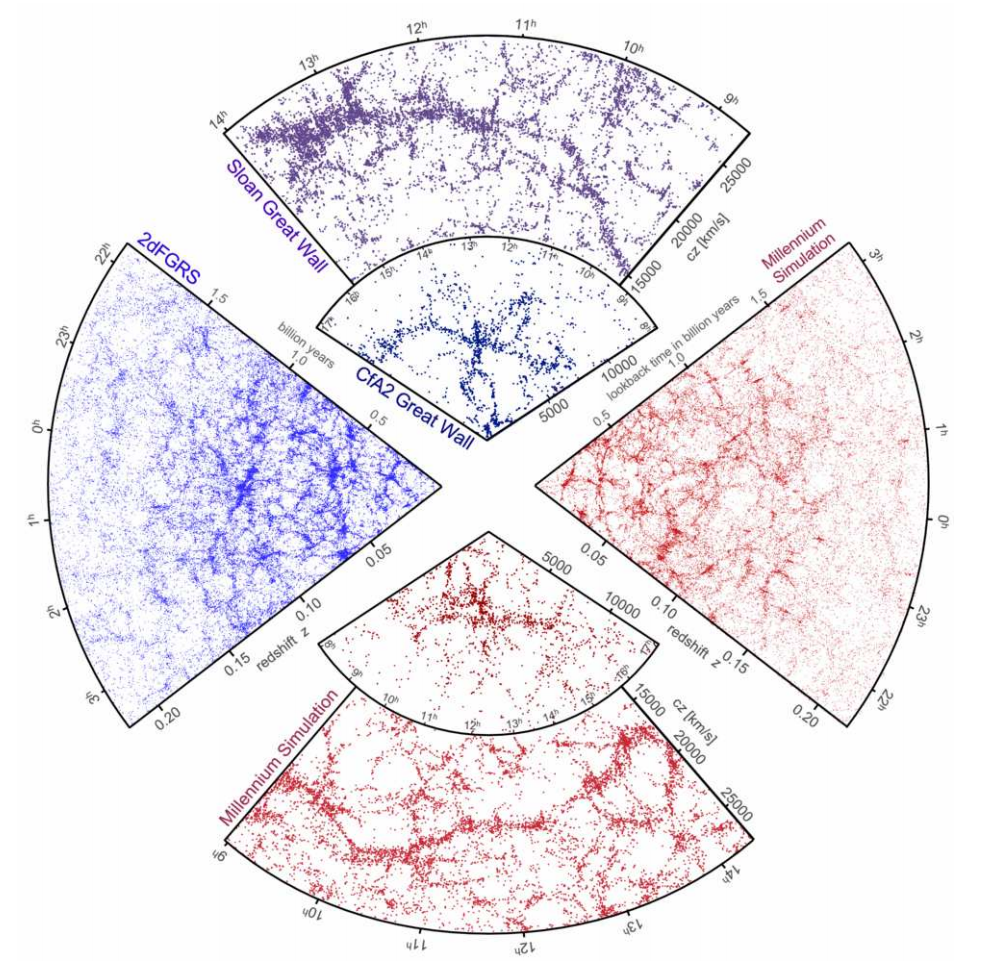
\includegraphics[width=\columnwidth]{figures/diagrams/mill_catalog_comparison.png}
\centering
\caption[]{A comparative diagram of Millennium simulation data against galaxy survey data\protect\footnotemark.}
\label{fig:gal_catalogs}
\end{figure}
\footnotetext{Image from \url{wwmpa.mpa-garching.mpg.de/millennium}.}

\subsection{Gravitational wave sources} % Rachel Gray et al. paper
Measurements of cosmological parameters from observations of gravitational wave events are independent of the 
electromagnetic (EM) spectrum and any obstacles to the transmission of EM radiation. Because these measurements 
do not use EM radiation, they provide alternative estimates that do not depend on cosmological distance 
scale~\cite{gw_distance_scale}. Information on dark energy density at $z>0.1$, past the edge of the local universe, 
could be obtained to better constrain cosmological parameters. At this distance, the cosmological distance-redshift 
relation depends on more than just $H_0$~\cite{gw_cosmology}. A further dependency is on the matter and dark energy 
densities $\Omega_m$ and $\Omega_\Lambda$. The values of these parameters could be constrained by measurements of the 
background rate of expansion from gravitational wave (GW) events at non-local redshifts. Next generation GW detectors 
such as Cosmic Explorer~\cite{cosmic_explorer} and the Einstein Telescope~\cite{einstein_telescope} as well as space 
based detectors such as LISA~\cite{lisa} will be at the forefront of such observations.
There are also gravitational waves from epochs in the early universe. These are known as relic gravitational waves and 
they can be attributed to GWs in the paradigm of quintessential inflation~\cite{relic_gws}. GW astrophysics has potential 
in the future to open new windows onto the conditions of the early universe.

Gravitational waves were first observed in 2015 with the detection of the binary black hole merger GW150914~\cite{gw_detection}.
A separate GW observation was of the binary neutron star merger event GW170817~\cite{GW170817} and later the optical 
redshift measurement of its electromagnetic counterpart, the host galaxy NGC4993~\cite{em_counterpart1, em_counterpart2}. 
This event was used to constrain the value of the Hubble constant $H_0$. The value of $H_0$ was found to be $H_0 = 
70^{+12}_{-8}\text{ km s}^{-1} \text{ Mpc}^{-1}$. This was the first application of gravitational wave sirens in 
obtaining cosmological parameters such as $H_0$. A separate analysis that improved on the X-ray and radio emission 
modelling from GW170817~\cite{GW170817_m2} obtained a value $H_0 = 74.0^{+11.5}_{-7.5}\text{ km s}^{-1} \text{ Mpc}^{-1}$. 
The consensus for the true value of $H_0$ from electromagnetic spectrum observations is a contentious issue. Assuming the 
$\Lambda \text{CDM}$ cosmology, the Planck experiment found a value of $H_0 =~ 67.4 \pm~0.5 \text{ km s}^{-1} 
\text{ Mpc}^{-1}$~\cite{planck}. 

\begin{figure}
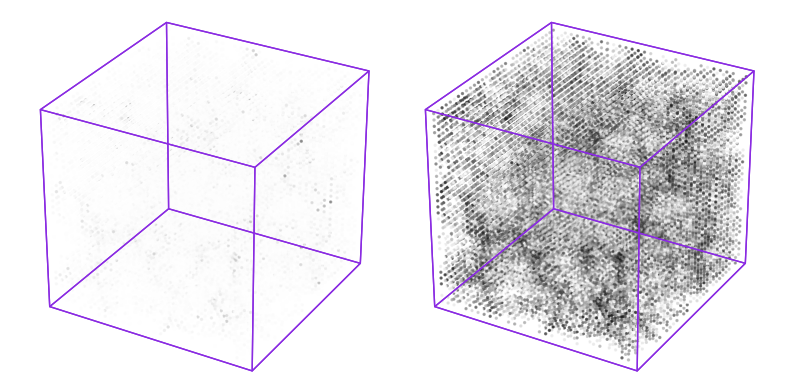
\includegraphics[width=\columnwidth]{figures/diagrams/scale_fig.png}% scaling2.png
\centering
\caption{The application of the scaling $s$ to a 3D-histogram training sample. The cube on the left shows an 
image $\mathbf{x}$ and on the right is a scaled image $s(\mathbf{x})$.}
\label{fig:scaling}
\end{figure}

The same event GW170817 had a degeneracy between the source distance and the viewing angle to the radio counterpart that 
limited the initial certainty in the EM localization of the GW source. This degeneracy was broken from radio 
interferometry~\cite{GW170817_source_radio} and a value of $H_0$ that disagrees with the previous values was found to be 
$68.9^{+4.7}_{-4.6} \text{ km s}^{-1} \text{ Mpc}^{-1}$~\cite{GW170817_jet_H0}. A recent survey calibrates Type Ia 
supernovae (SNe Ia) against a set of Tip of the Red Giant Branch (TRGB) stars~\cite{H0_redgiant}. These are bright stars
that have just initiated helium burning in their cores and $H_0$ from this calibration was found to be $69.8 \pm 0.8 \, 
(\pm1.1\% \text{ stat}) \pm 1.7 \, (\pm2.4\% \text{ sys})$. The disagreement between the competing values of $H_0$ could
be decided using more measurements from GW event observations and it is expected that accuracy similar to the level of
measurements by Planck is possible if between $10^6$ and $10^7$ gravitational wave events are 
observed~\cite{chris_planck_gw}.

Gray et al. 2019~\cite{gray} consider GW observations where the electromagnetic counterpart to the GW source is
unobservable so the distance to the electromagnetic counterpart is inferred as well as the GW source distance. This 
may become the norm for future searches into narrowing the uncertainties on cosmological parameters. The paper 
describes Bayesian methods used to obtain posteriors on $H_0$ from GW events.

The process involves the creation of a series of mock data challenges (MDCs). The MDCs are simulations of GW events 
in mock galaxy catalogues. Between the separate MDCs there are varying conditions of GW and EM selection effects 
(GW selection effects correspond to detector sensitivity and EM effects are due to observed flux limitations). The 
effects of clustering and large scale cosmological structure are ignored in the simulation of co-moving volumes of 
uniformly distributed galaxies that the GW events occur in. These mock catalogs show different comparisons to 
certain properties of true galaxy distributions from surveys for locating GW events, such as GLADE~\cite{GLADE}. %For 
% the complete galaxy catalogue in one such MDC a uniform simulated distribution of galaxies is added past the limit 
% of the catalog. 
A larger testing volume could be generated from a routine, such as the one described in this report, with the summary 
statistics that are similar to survey or simulation data with added realistic cosmological structure. The EM 
information from outside the volume specified in the catalogs could not be replaced by the GAN method shown in this 
report because at present it only returns positional data. This could increase the understanding of how current 
techniques for observed GW events perform so that tighter constraints on the source-observer separation could be 
obtained in the future. This would help to accumulate more data for posteriors to further constrain $H_0$.

% \begin{figure}[hbt!]
% 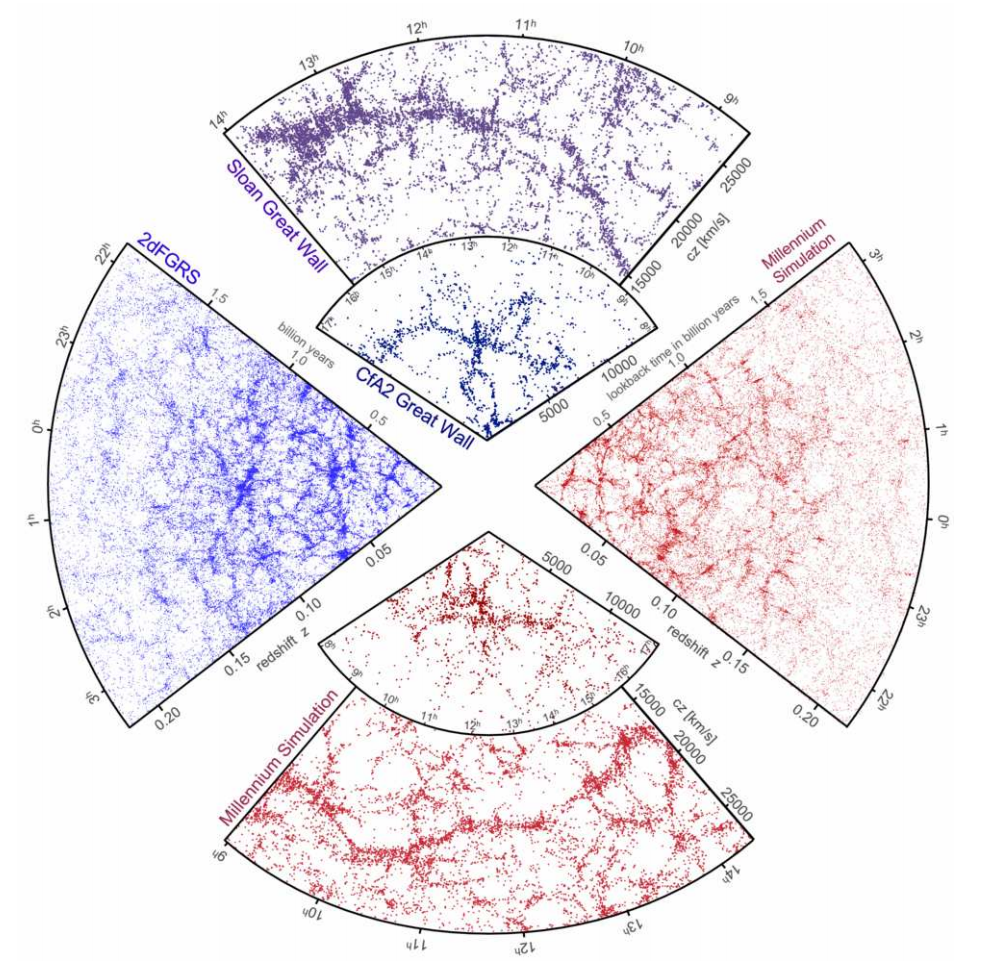
\includegraphics[width=\columnwidth]{figures/diagrams/mill_catalog_comparison.png}
% \centering
% \caption[]{A comparative diagram of Millennium simulation data against galaxy survey data\protect\footnotemark.}
% \label{fig:gal_catalogs}
% \end{figure}
% \footnotetext{Image from \url{wwmpa.mpa-garching.mpg.de/millennium}.}

In short, expanding the range for credible inferences of GW event localizations with increased understanding of GW event 
analyses would provide a more accurate estimate on the value of $H_0$ and other important parameters. This will be 
important in the next runs of LIGO~\cite{future_ligo}. The completed runs have already shown the higher frequency of 
binary black holes found at larger distances compared to binary neutron stars~\cite{GW_BNS_BBH_catalog}, where current 
galaxy catalogs are incomplete. The true substitute of the incompleteness could be replaced by a fast and realistic 
simulation from a conditional generative model that is given a redshift value. It should be noted that there is no reason
such a generative model could not generalise to higher redshift simulation data for this purpose. This is left to the 
discussion of future work in Section~\ref{sec:future_work}. This idea shows the direct link between generative AI and 
new discoveries in astrophysics.

\begin{figure}[!ht]%[hbt!]
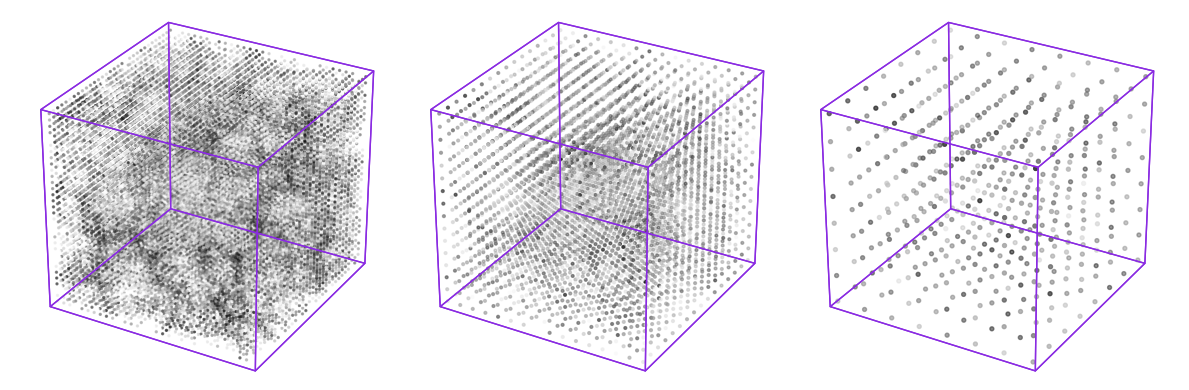
\includegraphics[width=\columnwidth]{figures/diagrams/kernel_fig.png}
\centering
\caption{A histogram down-sampled with three kernels of size $k=\{1, 2, 4\}$ (from left to right).}
\label{fig:kernel_fig}
\end{figure}

%%%%%%%%%%%%%%%%%%%%%%%%%%%%%%%%%%%%%%%%%%%%%%%%%%%%%%%%%%%%%%%%%%%%%%%%%%%%%%%%%%%%%%%%%%%%%%%%%%%%%%%%%%%%%%%%%%%%%%%%%%%
%%%%%%%%%%%%%%%%%%%%%%%%%%%%%%%%%%%%%%%%%%%%%%%%%%%%%%%%%%%%%%%%%%%%%%%%%%%%%%%%%%%%%%%%%%%%%%%%%%%%%%%%%%%%%%%%%%%%%%%%%%%
%%%%%%%%%%%%%%%%%%%%%%%%%%%%%%%%%%%%%%%%%%%%%%%%%%%%%%%%%%%%%%%%%%%%%%%%%%%%%%%%%%%%%%%%%%%%%%%%%%%%%%%%%%%%%%%%%%%%%%%%%%%

\section{Methods}\label{sec:methods}

%%%%%%%%%%%%%%%%%%%%%%%%%%%%%%%%%%%%%%%%%%%%%%%%%%%%%%%%%%%%%%%%%%%%%%%%%%%%%%%%%%%%%%%%%%%%%%%%%%%%%%%%%%%%%%%%%%%%%%%%%%%
%%%%%%%%%%%%%%%%%%%%%%%%%%%%%%%%%%%%%%%%%%%%%%%%%%%%%%%%%%%%%%%%%%%%%%%%%%%%%%%%%%%%%%%%%%%%%%%%%%%%%%%%%%%%%%%%%%%%%%%%%%%

\subsection{Simulation data}
% Basic intro to Cosmology simulations, describe simulation being used, redshift details
Hydrodynamical simulations of particles with masses on the order of a typical galaxy are the best way to emulate 
cosmological phenomena for testing without observational complications. Cosmological simulations model the physics in 
the evolution of baryonic and dark-matter in a self-consistent way that does not depend on observations.

The Millennium Project Simulation was used to sample training data for the generative models. The Millennium simulation
was published in 2005 by Springel et al.~\cite{millsim} and remains active in research today. The simulation was run 
using the GADGET2 code~\cite{gadget2} and it contains $2160^3$ particles of mass $8.6 \times 10^8 \, h^{-1}  \, M_{Sun}$ 
in a box of side length $512  \: h^{-1} \,\textup{Mpc}$. The cosmological parameters of the Millennium simulation are 
based on WMAP-1 data~\cite{wmap1} and the 2dF Galaxy Redshift Survey~\cite{2df}. These are $\Omega_m=0.25$, 
$\Omega_{\Lambda}=0.75$, $\Omega_b=0.045$ and $h=0.73$. Figure \ref{fig:gal_catalogs} shows a comparison of the 
Millennium simulation to the large scale structure and redshifts of the 2dF Galaxy Redshift Survey. 

The galaxy catalogs containing physical properties of galaxies in the Millennium simulation were derived with the 
Semi-Analytic Galaxy Evolution (SAGE) codebase by Croton et al. 2016~\cite{Croton2016} that improves on the earlier 
model of Croton et al. 2006~\cite{Croton2006}. The SAGE catalogs were sourced from the Theoretical Astrophysical 
Observatory (TAO)~\cite{TAO}. SAGE modelling adds baryonic processes into N-body simulations of halos after the 
simulations have been run. The baryonic particle properties are from information in the simulation run such as mass, 
size, spin and their merger history. SAGE models account for different mechanisms that affect the evolutions of 
galaxies and therefore the evolution of cosmological structure. The N-body particle positions of the Millennium-SAGE 
data were taken from snapshots at discrete redshifts $z=\{0.00, 1.07, 2.07, 3.06, 4.18, 5.28\}$ to give the training 
data for the ACGAN. 

%%%%%%%%%%%%%%%%%%%%%%%%%%%%%%%%%%%%%%%%%%%%%%%%%%%%%%%%%%%%%%%%%%%%%%%%%%%%%%%%%%%%%%%%%%%%%%%%%%%%%%%%%%%%%%%%%%%%%%%%%%%
%%%%%%%%%%%%%%%%%%%%%%%%%%%%%%%%%%%%%%%%%%%%%%%%%%%%%%%%%%%%%%%%%%%%%%%%%%%%%%%%%%%%%%%%%%%%%%%%%%%%%%%%%%%%%%%%%%%%%%%%%%%

\subsection{Extraction of training data} 
% TRAINING DATA AND PREPROCESSING
Position vector components for the centres of cube samples in the simulation volume were drawn from a uniform distribution 
along each axis of each redshift-snapshot. If the addition or subtraction of half the side length of the cube to any of 
the components resulted in a point outside of the simulation volume, the point was discarded. The galaxy cube samples were 
obtained by sorting the position vectors of galaxies in the simulation that were within the cube volume. Each point inside 
the cube was recorded in an array. The data was augmented by rotating the simulation box through random Euler angles to 
extend the number of possible unique cubes. From each simulation volume of $512 \: h^{-1} \,\textup{Mpc}$ ensembles of 64 
array samples of size $200 \: h^{-1} \,\textup{Mpc}$ were selected. The galaxy positions in each array for every cube were 
scaled to the range $[-1,+1]$. 3D-histograms with 32 bins per axis were made on each cube across the same range for each 
axis. The densities in each bin cell were also scaled to this range to fit the output ranges of the GAN models. 
% After testing different sizes, a cube size of $160 \: h^{-1} \,\textup{Mpc}$ was found to balance the selection of unique 
% samples in the simulation volume against featuring the same features in the simulation structure.

% \begin{figure}
% 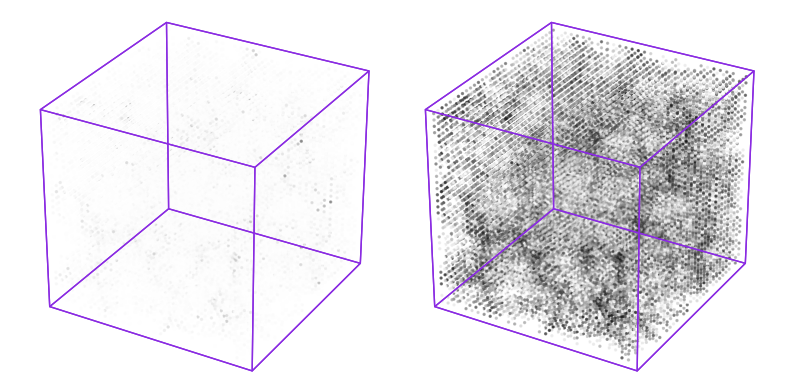
\includegraphics[width=\columnwidth]{figures/diagrams/scale_fig.png}% scaling2.png
% \centering
% \caption{The application of the scaling $s$ to a 3D-histogram training sample. The cube on the left shows an 
% image $\mathbf{x}$ and on the right is a scaled image $s(\mathbf{x})$.}
% \label{fig:scaling}
% \end{figure}

%%%%%%%%%%%%%%%%%%%%%%%%%%%%%%%%%%%%%%%%%%%%%%%%%%%%%%%%%%%%%%%%%%%%%%%%%%%%%%%%%%%%%%%%%%%%%%%%%%%%%%%%%%%%%%%%%%%%%%%%%%%
%%%%%%%%%%%%%%%%%%%%%%%%%%%%%%%%%%%%%%%%%%%%%%%%%%%%%%%%%%%%%%%%%%%%%%%%%%%%%%%%%%%%%%%%%%%%%%%%%%%%%%%%%%%%%%%%%%%%%%%%%%%

\subsection{Initial data transformations} 
The 3D-histograms have pixel densities that span across many orders of magnitude from voids to dense clusters of galaxies 
for each redshift value. The origin of GANs from image generation tasks has optimised the various architectures present in 
the literature for the general statistical structure of these images - the pixel densities in natural images are typically 
more uniformly distributed over the same scales. To help the GAN in generating sparsely distributed densities a transform, 
first utilised in~\cite{web_gan}, was used on the histograms to enhance the contrast between the density features. The 
transform from the original histogram $\mathbf{x}$ to the scaled histogram $s(\mathbf{x})$ is 

\begin{equation}
    s(\mathbf{x}) = \frac{\mathbf{x} - a}{\mathbf{x} + a}
\end{equation}

where $a$ is a free parameter that depends on the sparsity of the histogram densities. This is applied element-wise across 
the training data for all redshifts $z$. The value of $a=1.25$ was found to be optimal for the 
$200 \:  \: h^{-1} \,\textup{Mpc}$ histograms at all redshifts $z$. This parameter remains fixed during training. The value 
of $a$ controls the median pixel density of the scaled image. Figure \ref{fig:scaling} shows the difference between scaled 
images $s(\mathbf{x})$ and the original images $\mathbf{x}$. The inverse transformation $s^{-1}(\mathbf{x})$ can be applied 
to obtain the original image. 

% A logarithmic scaling was used originally, but this did not provide good results with the GAN architecture that used 
% the hyperbolic tangent ($\tanh$) activation because the logarithm of a negative number is undefined. The models using 
% $\tanh$ activations achieved much better results than models without these activations.

%%%%%%%%%%%%%%%%%%%%%%%%%%%%%%%%%%%%%%%%%%%%%%%%%%%%%%%%%%%%%%%%%%%%%%%%%%%%%%%%%%%%%%%%%%%%%%%%%%%%%%%%%%%%%%%%%%%%%%%%%%%
%%%%%%%%%%%%%%%%%%%%%%%%%%%%%%%%%%%%%%%%%%%%%%%%%%%%%%%%%%%%%%%%%%%%%%%%%%%%%%%%%%%%%%%%%%%%%%%%%%%%%%%%%%%%%%%%%%%%%%%%%%%

\subsection{Networks, architectures and training}\label{training}

% \subsubsection{2D-GAN implementation} % DESCRIBE SPECIFICS OF THIS IMPLEMENTATION
% \textit{Architecture} --- 
% The networks follow the structuring of the DCGAN models~\cite{dcgan} and are written in Keras~\cite{keras}. A full 
% description of the layers in the 2D-GAN architecture is given in Table~\ref{table:2dgan_archi} of 
% Appendix~\ref{appendix:gan_setups}. The generator transforms a 100-dimensional vector drawn from a Gaussian prior 
% $\mathbf{z}\sim \mathcal{N} (0,1)$ into a $32\times 32$ single-channel image. The latent-space vector is followed by a 
% fully connected layer that is reshaped to a stack of feature maps for the two convolutional layers. Batch-normalisation 
% is only used after the fully connected layer. Through each layer hyperbolic tangent activations are used. See 
% Appendices~\ref{appendix:app_acts} and~\ref{app_BN} for more detail on batch-normalisation and activation functions. 

% The discriminator network has two convolutional layers and two fully connected layers. The image samples have features 
% extracted by the first two convolutional layers and the features are flattened for the final fully connected layers. 
% Hyperbolic tangent functions are used throughout the model and a sigmoid activation function (see 
% Appendix~\ref{appendix:app_acts}) is used for the final single neuron layer that outputs the probability for a given 
% sample being real. 

% Both networks use the same number of filters for the corresponding layers in either model. Together the discriminator 
% and generator models have $3.8\times 10^7$ trainable parameters. The discriminator and generator objectives of 
% Equations~\ref{eq:J_D} and \ref{eqn:J_G} are minimized using the Adam optimiser~\cite{adam}. Each model uses a learning 
% rate of $2\times 10^{-4}$ and momentum $\beta_1 = 0.5$. The models use a batch size of 64 histograms out of a set of 128 
% training histograms, where the batch size is the number of samples given to the discriminator at each iteration of 
% training. Refer to Table~\ref{table:2dgan_params} of Appendix~\ref{appendix:gan_setups} for a complete listing of the 
% 2D-GAN hyper-parameters used in each model. The hyper-parameters of a model are set outside of training and they shape 
% how the training proceeds.\\

% {\setlength{\parindent}{0cm}
% \textit{Training} --- GANs are notoriously difficult to train. This means that the state of the models can generate 
% realistic samples for a single epoch at a time. The GAN was made to record the parameters of the generator model at 
% these epochs by using a statistical check (see Section~\ref{sec:stats_and_diags}) of the generated histograms against 
% the training data histograms in the training loop. The loss (the objective function value) and accuracy values of the 
% discriminator for each epoch were recorded during training.
% % }

% % An indicator for the performance of a GAN is the classification accuracy of the discriminator model. This metric is 
% the average classification accuracy of the discriminator on two separate batches of real and fake samples. The accuracy 
% metric for the generator is given by the same accuracy subtracted from one. However, in this case the accuracy is the 
% discriminator's accuracy in classifying a batch of fake cubes labelled as real. This is because the generator is trying 
% to make the discriminator classify its products as real. The best results were obtained when the losses of the networks 
% diverged and the accuracies of the networks slowly increased and were at approximately the same value. A training loop 
% of $3.0\times 10^4$ epochs for the $80\:h^{-1} \textup{ Mpc}$ cubes sectioned into $32 \times 32$ pixel projections 
% took approximately 2 hours on an NVIDIA Tesla V100 GPU with 32GB capacity.

% % \begin{figure*}[!ht]%[hbt!]
% % 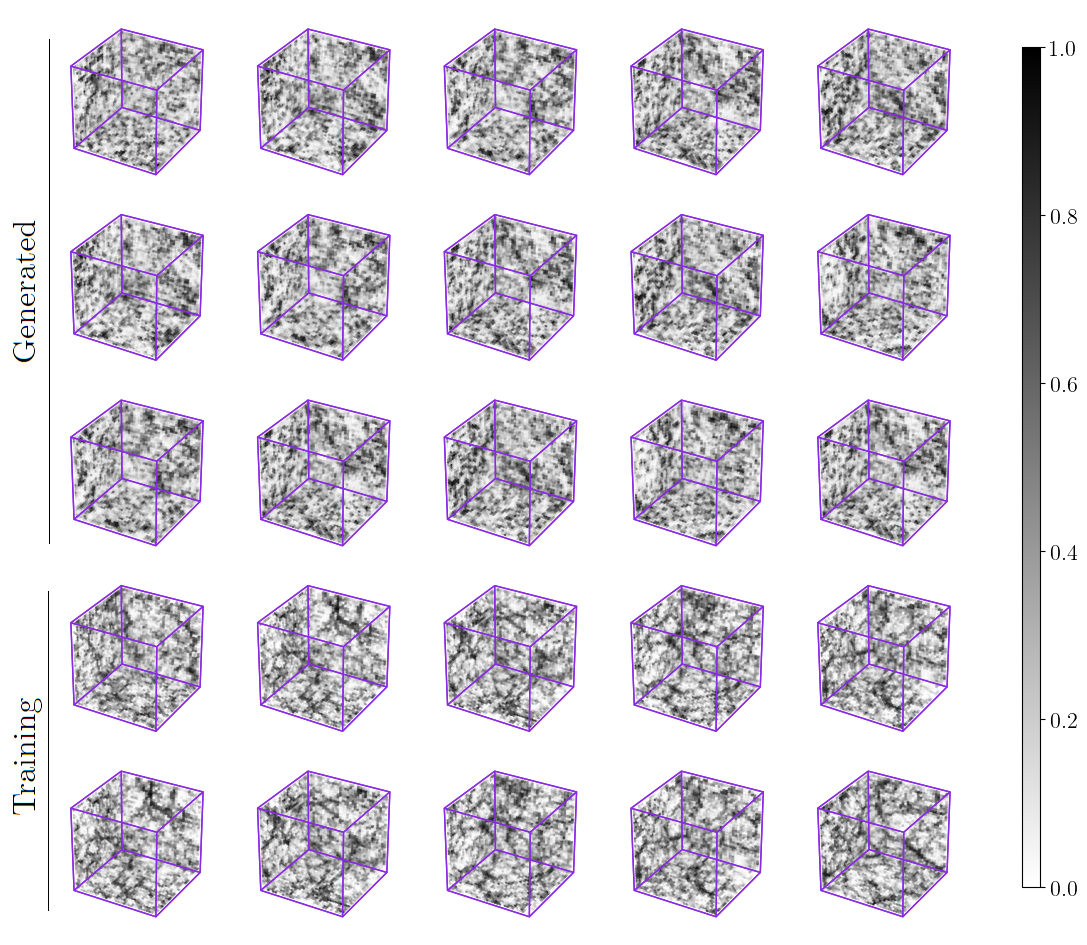
\includegraphics[width=17cm]{figures/cubes/t_g_3d.png}
% % \centering
% % \caption{Training data histograms and GAN-generated histograms from the 3D-GAN implementation.}
% % \label{fig:3dgan_imgs}
% % \end{figure*}
% % \begin{figure*}[!ht]%[hbt!]
% % \label{fig:2dgan_imgs}
% % 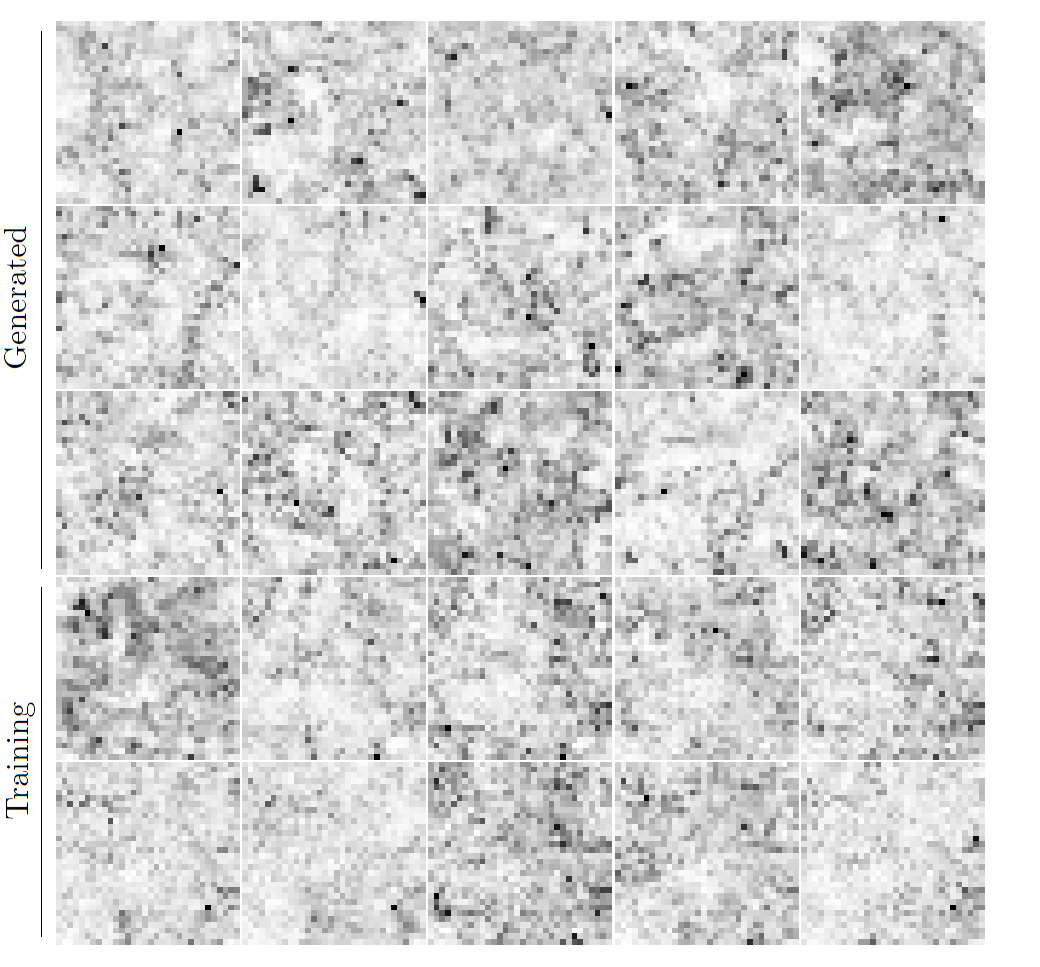
\includegraphics[width=16.5cm]{figures/cubes/t_g_2d.png}
% % \centering
% % \caption{Training data histograms and GAN-generated histograms from the 2D-GAN implementation.}
% % \label{fig:2dgan_imgs}
% % \end{figure*}

%%%%%%%%%%%%%%%%%%%%%%%%%%%%%%%%%%%%%%%%%%%%%%%%%%%%%%%%%%%%%%%%%%%%%%%%%%%%%%%%%%%%%%%%%%%%%%%%%%%%%%%%%%%%%%%%%%%%%%%%%%%

\subsubsection{Architecture}
Table~\ref{table:acgan_archi} of Appendix~\ref{appendix:acgan_setup} shows the architectures of the ACGAN discriminator 
and generator models. The hyper-parameters used in the ACGAN are also given in Table~\ref{table:acgan_params} of 
Appendix~\ref{appendix:acgan_setup}. Together the discriminator and generator models had around $2.5\times10^8$ trainable 
parameters across one linear layer and three convolutional layers for the generator model and three convolutional layers 
for the discriminator model. 
% \textit{Architecture} --- 
% Table~\ref{table:acgan_archi} of Appendix~\ref{appendix:acgan_setup} shows the architectures of the ACGAN discriminator 
% and generator models. The hyper-parameters used in the ACGAN are also given in Table~\ref{table:acgan_params} of 
% Appendix~\ref{appendix:acgan_setup}. Together the discriminator and generator models had around $2.5\times10^8$ trainable 
% parameters across one linear layer and three convolutional layers for the generator model and three convolutional layers 
% for the discriminator model. \\

% {\setlength{\parindent}{0cm}
% \textit{Training} --- 
% The networks follow the structuring of the DCGAN models~\cite{dcgan} and are written in Tensorflow~\cite{tensorflow} and 
% Keras~\cite{keras}. The generator transforms a 256-dimensional vector drawn from a Gaussian prior $\mathbf{z}\sim 
% \mathcal{N}(0,1)$ into a $32 \times 32 \times 32$ single-channel image. The latent-space vector is followed by a fully 
% connected layer that is reshaped to a stack of feature maps for the convolutional layers. 
% % Through each layer hyperbolic tangent activations are used. See Appendices~\ref{appendix:app_acts} and~\ref{app_BN} 
% % for more detail on batch-normalisation and activation functions. 
% }

%%%%%%%%%%%%%%%%%%%%%%%%%%%%%%%%%%%%%%%%%%%%%%%%%%%%%%%%%%%%%%%%%%%%%%%%%%%%%%%%%%%%%%%%%%%%%%%%%%%%%%%%%%%%%%%%%%%%%%%%%%%

\subsubsection{Training}

The networks follow the structuring of the DCGAN models~\cite{dcgan} and are written in Tensorflow~\cite{tensorflow} and 
Keras~\cite{keras}. The generator transforms a 256-dimensional vector drawn from a Gaussian prior $\mathbf{z}\sim 
\mathcal{N}(0,1)$ into a $32 \times 32 \times 32$ single-channel image. The latent-space vector is followed by a fully 
connected layer that is reshaped to a stack of feature maps for the convolutional layers. 
% Through each layer hyperbolic tangent activations are used. See Appendices~\ref{appendix:app_acts} and~\ref{app_BN} 
% for more detail on batch-normalisation and activation functions. 

The ACGAN implementation was limited by the GPU memory capacity - the parameters and architectures together with the 
sample batch sizes meant that the GPU was easily saturated. Deeper models with more convolutional units were implemented 
but these tended to stall the GPU. A training loop for $10^5$ epochs for the $200 \: h^{-1} \: \textup{Mpc}$ cubes 
formatted to $32 \times 32 \times 32$ pixel histograms took approximately 144 hours on an NVIDIA Tesla V100 GPU with 
32GB capacity. To augment the dataset with additional diversity for each redshift, the samples were rotated in-situ during 
training as the sample batches were gathered. 

Generative adversarial networks are harder to train with three-dimensional input data because of the increase in the 
number of configurations of interest in the data. There are a number of tricks and techniques for moving toward more 
convergent and stable training. A compilation of these has resulted from testing GANs in natural image tasks. The techniques
that were used to train the ACGAN in this work were one-sided label smoothing, historical averaging and a decaying noise 
input which were borrowed from~\cite{gantricks_sali, gan_noise_decay}. The exact implementations stem only from the 
original theoretical basis. One-sided label smoothing adds scalar values sampled from a uniform distribution $\mathcal{U}
(-0.1,0)$ to the real labels only. 
%Historical averaging~\cite{gantricks_sali} adds a penalty $L_H$ to the objective functions 
%of the discriminator and generator. The addition is

%\begin{equation}
%    L_H = \Bigl\lvert\Bigl\lvert \, \bm{\theta} - \frac{1}{t} \sum_i^t\bm{\theta}[i] \,  \Bigr\rvert\Bigr\rvert^2
%\end{equation}

%where $\bm{\theta}$ and $\bm{\theta}[i]$ are the model parameters at the present and previous epochs respectively. This
%cost term helps the networks avoid mode collapse. 
The decaying noise input temporarily slows the discriminator training
by showing it less clear real samples. This in turn allows a strong discriminator model that doesn't overwhelm the generator
early in training. The decaying noise input samples noise at each epoch to add to every histogram pixel in an ensemble of
samples. The Gaussian noise $\mathbf{n}$ has standard deviation $\sigma_i$ that depends on epoch $i$ such that 

\begin{equation}
    \mathbf{n} \sim \mathcal{N}(0,\sigma_i), \: \: \sigma_i = A \textup{e}^{-\gamma i}
\end{equation}

where the free parameters $A=10^{-2}$ and $\gamma=10^{-3}$ were found to work well. Diluting the real and fake batches of 
samples to $1\%$ of the batch-size with the opposite validity of samples helped the training process stabilise.

%%%%%%%%%%%%%%%%%%%%%%%%%%%%%%%%%%%%%%%%%%%%%%%%%%%%%%%%%%%%%%%%%%%%%%%%%%%%%%%%%%%%%%%%%%%%%%%%%%%%%%%%%%%%%%%%%%%%%%%%%%%

\subsubsection{Minibatch Discrimination}

Minibatch discrimination~\cite{gantricks_sali} was implemented to help avoid mode collapse by discriminating over a 
collection of samples given to the discriminator as opposed to a single sample at a time. The original work describes 
the `closeness' of samples in a collection as follows: Let $\mathbf{f}(\bm{x}_i) \in \mathbb{R}^A$ represent a vector of 
features extracted by $D$ for sample $\mathbf{x}_i$, where $A$ is the number of components of the feature vector. Multiplying $\mathbf{f}(\bm{x}_i)$ by a tensor $T \in \mathbb{R}^{A\times B\times C}$ results in a matrix $M_i^{B\times C}$, where $B$ 
and $C$ are the number of discriminative kernels and the dimensionality of the space where the closeness of samples is 
calculated. The $L_1$-distance is calculated between each row of $M_i$ for each sample $i$ in the collection. The distances 
are exponentiated as

\begin{equation}
    c_b(\mathbf{x}_i, \mathbf{x}_j) = \exp({- ||M_{i,b} - M_{j,b}||_{L_1}}) \in \mathbb{R} \nonumber
\end{equation}

The output $o(\mathbf{x}_i)$ of the minibatch discrimination layer for a sample $\mathbf{x}_i$ is defined as the sum of 
each $c_b(\mathbf{x}_i, \mathbf{x}_j)$ for $B$ samples in a minibatch

\begin{eqnarray}
    o(\mathbf{x}_i)_b &=& \sum_{j=1}^n c_b(\mathbf{x}_i, \mathbf{x}_j) \nonumber \\
    o(\mathbf{x}_i) &=& [o(\mathbf{x}_i)_1, o(\mathbf{x}_i)_2, ..., o(\mathbf{x}_i)_B] \in \mathbb{R}^B \nonumber\\
    % o(\mathbf{x}_i) &=& \sum_{b=1}^B o(\mathbf{x}_i)_b\\ 
    o(\mathbf{X}) &\in& \mathbb{R}^{n \times B} \nonumber
\end{eqnarray}

Where $n$ is the number of pairings in a minibatch and  $\mathbf{X}$ denotes a minibatch of samples. The minibatch 
discrimination output is concatenated to the 
flattened-features from the last convolutional layers in the discriminator. This is done separately for the real and 
fake samples. The discriminator is able to designate the validity of a sample with additional information from samples 
in a collection which in turn causes the generator to promote variety in its products.

%%%%%%%%%%%%%%%%%%%%%%%%%%%%%%%%%%%%%%%%%%%%%%%%%%%%%%%%%%%%%%%%%%%%%%%%%%%%%%%%%%%%%%%%%%%%%%%%%%%%%%%%%%%%%%%%%%%%%%%%%%%

\subsubsection{Spectral Normalization}
To control discriminator training and the heuristic feedback to the generator and its products, a method proposed by 
\cite{spectral_norm} uses the normalization of weight matrices in the discriminator and generator convolutional nets. This 
method allows control over the derivative of the discriminator value function in the adversarial setting of GANs. The 
Lipschitz constant of the discriminator is constrained without specifics concerning the inputs to either models. This 
data-independent regularization is an advantage over traditional regularization particularly in the generative context. 
The spectral norm of a weight matrix $W$ for a given layer $g : \mathbf{h}_{in} \rightarrow \mathbf{h}_{out}$ is

\begin{equation}
    \sigma(W) = \max_{\mathbf{h}:\mathbf{h}\neq 0} \frac{|| W \mathbf{h}||_2}{||\mathbf{h}||_2}
              = \max_{||\mathbf{h}||_2 \leq 1} ||W\mathbf{h}||_2
\end{equation}

which is equivalent to the singular value of $W$. This is applied to all layers in the discriminator and the generator.

%%%%%%%%%%%%%%%%%%%%%%%%%%%%%%%%%%%%%%%%%%%%%%%%%%%%%%%%%%%%%%%%%%%%%%%%%%%%%%%%%%%%%%%%%%%%%%%%%%%%%%%%%%%%%%%%%%%%%%%%%%%
%%%%%%%%%%%%%%%%%%%%%%%%%%%%%%%%%%%%%%%%%%%%%%%%%%%%%%%%%%%%%%%%%%%%%%%%%%%%%%%%%%%%%%%%%%%%%%%%%%%%%%%%%%%%%%%%%%%%%%%%%%%

\subsubsection{Auxiliary Classification}
The ACGAN uses a secondary classification model to designate the discriminators belief in the type of image it has been 
shown. This model is nothing more than a classification neural network that is connected to the feature-extracting 
convolutions of the discriminator model. The model is optimised together with the discriminator using a sparse categorical
cross entropy function that calculates the cross entropy between two one-hot-encoded classification vectors that pertain 
to the class of an image. In practice a softmax activation function is used, which defines a discrete probability 
distribution over the class labels for each redshift value. 
% This auxiliary classifier model is optimised and trained externally to the discriminator and generator models.

%%%%%%%%%%%%%%%%%%%%%%%%%%%%%%%%%%%%%%%%%%%%%%%%%%%%%%%%%%%%%%%%%%%%%%%%%%%%%%%%%%%%%%%%%%%%%%%%%%%%%%%%%%%%%%%%%%%%%%%%%%%
%%%%%%%%%%%%%%%%%%%%%%%%%%%%%%%%%%%%%%%%%%%%%%%%%%%%%%%%%%%%%%%%%%%%%%%%%%%%%%%%%%%%%%%%%%%%%%%%%%%%%%%%%%%%%%%%%%%%%%%%%%%
\subsection{Generating a universe}

%%%%%%%%%%%%%%%%%%%%%%%%%%%%%%%%%%%%%%%%%%%%%%%%%%%%%%%%%%%%%%%%%%%%%%%%%%%%%%%%%%%%%%%%%%%%%%%%%%%%%%%%%%%%%%%%%%%%%%%%%%%

% {\setlength{\parindent}{0cm}
% \textit{Redshift interpolation} --- 
% To observe the A fixed point in the latent space is chosen and 
% }
\subsubsection{Redshift interpolation}\label{methods:z_interp}
% talk about what this is in our method, what comes out of doing it 
The latent space of a generator in a typical GAN framework stores a compressed representation of the statistical structure
of the distribution of the real data. By choosing different points in this space and supplying them to the generator, 
samples can be derived with different characteristics that have been extracted from the training process of the 
discriminator and generator models.

An array of latent-space vectors and class labels of a given redshift are passed to the trained ACGAN generator to create
a collection of cube samples. 
%These are placed together face-to-face to create larger samples of cosmic structure. A 
%discussion on the viability of this approach is left to Section~\ref{sec:results}.
In the specific case of interpolating through redshift $z$ values, a single point in the latent-space was chosen. This was 
repeatedly supplied to the generator with a class label $c$ that was changed by a small amount $\textup{d}c \sim 0.01$. 
This demonstrates the understanding of the generative model on the relationship between realisations of cosmic structure 
at different values of $z$. The results of this are left to Section~\ref{sec:results}.
% might be bad because of not enough training data, normalisation, parameter capacity in G, z-dim value

%%%%%%%%%%%%%%%%%%%%%%%%%%%%%%%%%%%%%%%%%%%%%%%%%%%%%%%%%%%%%%%%%%%%%%%%%%%%%%%%%%%%%%%%%%%%%%%%%%%%%%%%%%%%%%%%%%%%%%%%%%%

% \subsubsection{Latent space navigation}\label{methods:z_navig}
% % show the maths behind it, the general method of doing it. See https://arxiv.org/pdf/1609.04468.pdf, % (Larsen et al., 2016).
% In all non-trivial cases, the number of parameters available to the generative model of a GAN through its architecture is 
% less than the total parameters that constitute the training set. This means the discriminator and generator must find 
% condensed representations of the training data. The generator model is sampled from a set of latent variables in the 
% latent space that constitute the latent-vectors $\mathbf{z}$. Vector space arithmetic with points in the latent space 
% allows interpolation between tenable examples of learned representations of the training data the GAN is exposed to in 
% training. 
% % With the inherent structuring of the latent space by GANs, these operations can allow complex 

% Interpolation is the transit between two distinct points in the latent space. In this work, spherical interpolation is used
% as opposed to linear interpolation. The latter being a over-simplistic approach as the latent space of the model trained in
% this work had 256 dimensions with a Gaussian prior $\mathcal{N}(0,1)$. Spherical interpolation~\cite{spherical_interp} uses 
% a great circle arc on the N-dimensional hypersphere in the latent space, with a path given by 

% \begin{equation}
%     S(q_1, q_2; \mathbf{\mu}) = \frac{\sin (1 - \mu)\theta}{\sin \theta}q_1 + \frac{\sin \mu\theta}{\sin \theta}q_2
% \end{equation}

% where a discrete set of points between points $q_1$ and $q_2$ are passed to the generator model to create samples~with and
% $\mu$ are the discrete proportioned steps between $q_1$ and $q_2$. It should be noted that simple linear interpolation 
% along a given axis of the latent space would disregard the curvature of the 256-dimensional latent space and so the path 
% along a great circle by spherical interpolation is required.

%% In these cases, we have performed a linear interpolation which assumes that the latent space is uniformly distributed 
%% hypercube. Technically, our chosen latent space is a 100-dimension hypersphere or multimodal Gaussian distribution.

%%%%%%%%%%%%%%%%%%%%%%%%%%%%%%%%%%%%%%%%%%%%%%%%%%%%%%%%%%%%%%%%%%%%%%%%%%%%%%%%%%%%%%%%%%%%%%%%%%%%%%%%%%%%%%%%%%%%%%%%%%%

% \subsubsection{Building larger volumes from generated samples}\label{methods:volume_building}
% % say how the larger volumes are made from smaller generated cubes, talk about 
% A selection of cubes were generated with a batch of $N$ latent vectors $\mathbf{Z}=\{\mathbf{z}_i, ..., \mathbf{z}_N\}$ 
% drawn from the same prior $\mathcal{N}(0,1)$ as the generative model in training. These are placed at points on a cubic 
% mesh to create a larger box of generated cubes. This was repeated for side-lengths 7, 9 and 11 (in multiples of the initial 
% generated cube side-lengths). 

%%%%%%%%%%%%%%%%%%%%%%%%%%%%%%%%%%%%%%%%%%%%%%%%%%%%%%%%%%%%%%%%%%%%%%%%%%%%%%%%%%%%%%%%%%%%%%%%%%%%%%%%%%%%%%%%%%%%%%%%%%%
%%%%%%%%%%%%%%%%%%%%%%%%%%%%%%%%%%%%%%%%%%%%%%%%%%%%%%%%%%%%%%%%%%%%%%%%%%%%%%%%%%%%%%%%%%%%%%%%%%%%%%%%%%%%%%%%%%%%%%%%%%%
%%%%%%%%%%%%%%%%%%%%%%%%%%%%%%%%%%%%%%%%%%%%%%%%%%%%%%%%%%%%%%%%%%%%%%%%%%%%%%%%%%%%%%%%%%%%%%%%%%%%%%%%%%%%%%%%%%%%%%%%%%%

\section{Statistics and diagnostics}\label{methods:stats_and_diags}
% WHAT ARE THESE MEASURES FOR? WHY ARE THEY IMPORTANT TO THE EXPERIMENT ? 
% WHAT DO THE STATS CONSIST OF IN MAKING? WHAT DO THEY SHOW?

\subsection{Comparison of distributions with Kullback-Leibler Divergences}
Generative Adversarial Networks reduce the difference of the model probability distribution between the generated samples 
$p_{model}$ and the probability distribution of the training data samples $p_{data}$. This reduction quantifies how well 
$p_{model}$ estimates $p_{data}$. An estimate on the suitability of this replacement was made using a comparison with 
different ensembles of samples. The ensembles were collected from the training, generated and uniform distributions of 
histograms denoted $t$, $g$ and $u$ at each redshift $z$. The uniform distribution $u$ was a set of histograms with pixel 
densities drawn from a uniform distribution $\mathcal{U}(-1,1)$ so the samples are not discriminated for a redshift value 
in any comparison. The comparison of sample ensembles tested how well the generator made the discriminator associate the 
real and generated samples to the same distribution. The Kullback-Leibler (KL) divergence and its relevance to the 
comparisons is defined in Appendix~\ref{appendix:kl_div}.

% \begin{figure}[!ht]%[hbt!]
% 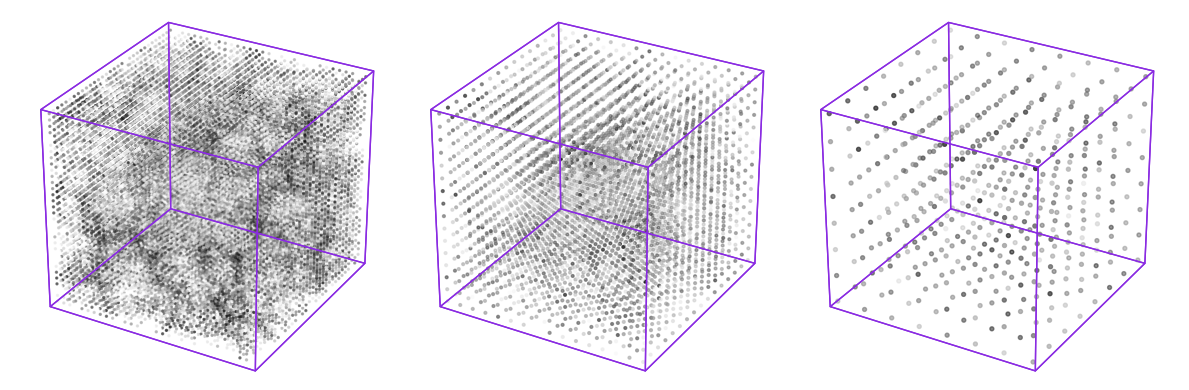
\includegraphics[width=\columnwidth]{figures/diagrams/kernel_fig.png}
% \centering
% \caption{A histogram down-sampled with three kernels of size $k=\{1, 2, 4\}$ (from left to right).}
% \label{fig:kernel_fig}
% \end{figure}

\begin{figure}
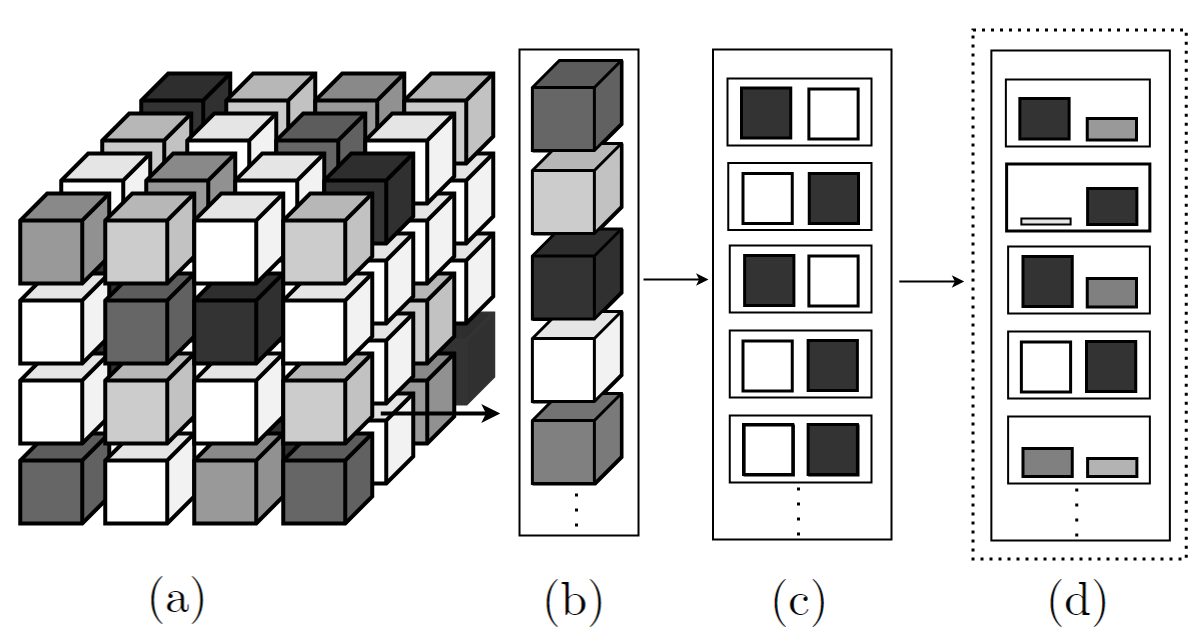
\includegraphics[width=\columnwidth, trim=4 4 4 4,clip]{figures/diagrams/kl_stat_process1.png}
\centering
\caption{From a single ensemble of 3D-histograms to a normalised distribution; 
         (a) - an ensemble of 3D-histograms that will be transformed into a distribution, 
         (b) - the flattened vector of bin-cells, 
         (c) - the histograms of each vector-component, 
         (d) - the final collapsed vector encoding the whole of a given distribution of 3D-histograms.}
\label{fig:klstat}
\end{figure}

%%%%%%%%%%%%%%%%%%%%%%%%%%%%%%%%%%%%%%%%%%%%%%%%%%%%%%%%%%%%%%%%%%%%%%%%%%%%%%%%%%%%%%%%%%%%%%%%%%%%%%%%%%%%%%%%%%%%%%%%%%%
%%%%%%%%%%%%%%%%%%%%%%%%%%%%%%%%%%%%%%%%%%%%%%%%%%%%%%%%%%%%%%%%%%%%%%%%%%%%%%%%%%%%%%%%%%%%%%%%%%%%%%%%%%%%%%%%%%%%%%%%%%%

\subsubsection{Histogram distributions}
Distributions of training and generated samples were gathered for each redshift $z$ and the average relative entropy 
between the ensembles was calculated to estimate how similar the generated and simulation samples were to each other.
The uniform distribution $u$ was made to have samples to compare with that did not have any correlated structure on any 
scale. The comparison of ensembles shows the spread of the $D_{KL}$ value on samples from the original distributions $t$, 
$g$ and $u$ and consequently how different random groups of samples are to each other. In the case of the uniform-training 
and uniform-generated comparisons it shows how similar the samples are to a uniform distribution. The $D_{KL}$ values 
between draws of samples from distributions $a$ and $b$ were calculated for both $D_{KL}(a||b)$ and $D_{KL}(b||a)$. 

%%%%%%%%%%%%%%%%%%%%%%%%%%%%%%%%%%%%%%%%%%%%%%%%%%%%%%%%%%%%%%%%%%%%%%%%%%%%%%%%%%%%%%%%%%%%%%%%%%%%%%%%%%%%%%%%%%%%%%%%%%%
%%%%%%%%%%%%%%%%%%%%%%%%%%%%%%%%%%%%%%%%%%%%%%%%%%%%%%%%%%%%%%%%%%%%%%%%%%%%%%%%%%%%%%%%%%%%%%%%%%%%%%%%%%%%%%%%%%%%%%%%%%%

\subsubsection{Deriving the KL comparative diagnostic}
There were 32 samples in the ensembles from the distributions $t$, $g$ and $u$ that contained 64 samples each for each $z$ 
value. Each histogram in the ensemble was down-sampled by iterating a kernel of size $k$ over each histogram and summing 
the densities. The summed densities were divided by the number of bins in the kernel after down-sampling. This is equivalent 
to the initial histograms having a lower sampling with larger bins. After an ensemble is down-sampled, the ensembles of two 
distributions are compared. The samples are individually flattened to `histogram-vectors' with $(32/k)^3$ components. 
This is shown in Figure~\ref{fig:kernel_fig}. One-dimensional histograms with two bins were made for each component in the 
histogram-vectors. The two bins represented `high' and `low' pixel densities and the boundary between them was the median 
of the training data pixel densities. This is because using the median meant that it was not assumed that the pixel density 
distributions were symmetric. The histogram-vectors were then collapsed over the ensemble and normalised to sum to one as 
a probability distribution. The vector was then sampling the probability density function of pixel density. This process 
is illustrated in Figure \ref{fig:klstat}.

The distributions were compared with all the possible pairings of the set the distributions $\{ t, g, u\}$. The relative 
entropy, that is equivalent here to the KL divergence $D_{KL}$, was calculated between the distribution ensembles. The 
process was repeated for 100 separate ensembles and with the final $D_{KL}$ values logarithmically-scaled $D_{KL}$ 
histograms for each comparison were made. This process was repeated for each kernel size $k$ where $k \in \{1, 2, 4\}$.


%%%%%%%%%%%%%%%%%%%%%%%%%%%%%%%%%%%%%%%%%%%%%%%%%%%%%%%%%%%%%%%%%%%%%%%%%%%%%%%%%%%%%%%%%%%%%%%%%%%%%%%%%%%%%%%%%%%%%%%%%%%
%%%%%%%%%%%%%%%%%%%%%%%%%%%%%%%%%%%%%%%%%%%%%%%%%%%%%%%%%%%%%%%%%%%%%%%%%%%%%%%%%%%%%%%%%%%%%%%%%%%%%%%%%%%%%%%%%%%%%%%%%%%
\subsection{Power spectrum correlation}
% I have a code to generate power spectra for a set of cubes. compare training / generated / uniform spectra?


%%%%%%%%%%%%%%%%%%%%%%%%%%%%%%%%%%%%%%%%%%%%%%%%%%%%%%%%%%%%%%%%%%%%%%%%%%%%%%%%%%%%%%%%%%%%%%%%%%%%%%%%%%%%%%%%%%%%%%%%%%%
%%%%%%%%%%%%%%%%%%%%%%%%%%%%%%%%%%%%%%%%%%%%%%%%%%%%%%%%%%%%%%%%%%%%%%%%%%%%%%%%%%%%%%%%%%%%%%%%%%%%%%%%%%%%%%%%%%%%%%%%%%%
%%%%%%%%%%%%%%%%%%%%%%%%%%%%%%%%%%%%%%%%%%%%%%%%%%%%%%%%%%%%%%%%%%%%%%%%%%%%%%%%%%%%%%%%%%%%%%%%%%%%%%%%%%%%%%%%%%%%%%%%%%%

\section{Results}\label{sec:results}

%%%%%%%%%%%%%%%%%%%%%%%%%%%%%%%%%%%%%%%%%%%%%%%%%%%%%%%%%%%%%%%%%%%%%%%%%%%%%%%%%%%%%%%%%%%%%%%%%%%%%%%%%%%%%%%%%%%%%%%%%%%
%%%%%%%%%%%%%%%%%%%%%%%%%%%%%%%%%%%%%%%%%%%%%%%%%%%%%%%%%%%%%%%%%%%%%%%%%%%%%%%%%%%%%%%%%%%%%%%%%%%%%%%%%%%%%%%%%%%%%%%%%%%


\subsection{Generated images}
% show generated images at various redshifts, compare with training data
Figures~\ref{fig:t_z_imgs} and ~\ref{fig:g_z_imgs} show separate collections of simulated cosmic web and GAN-generated 
cosmic web for each class of redshift in the Millennium-SAGE training data. Across each value of redshift the ACGAN 
demonstrates its ability to evaluate each point in the latent space to a strong representation of a sample at the equivalent
redshift drawn from the model distribution. The ACGAN replicates the pixel density statistics well but the main downfall is 
in the reproduction of filament structure in the generated images. Typically the generated filaments are not as thin as their 
real counterparts in the training data. 

Across the generated samples there is no evidence of generator mode collapse whereby a small set of characteristics are 
reproduced across the generated samples. They show as much mutual difference as the training images.

%%%%%%%%%%%%%%%%%%%%%%%%%%%%%%%%%%%%%%%%%%%%%%%%%%%%%%%%%%%%%%%%%%%%%%%%%%%%%%%%%%%%%%%%%%%%%%%%%%%%%%%%%%%%%%%%%%%%%%%%%%%

\begin{figure*}[hbt!]
\includegraphics[width=17cm]{figures/cubes/acgan_training.png} % acgan3d_t_fig.png
\centering
\caption{A collection of training data cubes extracted from the Millennium-SAGE catalogs. Each row corresponds to the 
         redshift value given above each cube. The scaling $s(\mathbf{x})$ is applied to each cube $\mathbf{x}$.}
\label{fig:t_z_imgs}
\end{figure*}

\begin{figure*}[hbt!]
\includegraphics[width=17cm]{figures/cubes//acgan_generated.png} % acgan3d_g_fig.png
\centering
\caption{A collection of training data cubes extracted from the Millennium-SAGE catalogs. Each row corresponds to the 
         redshift value given above each cube. The scaling $s(\mathbf{x})$ is applied to each cube $\mathbf{x}$.}
\label{fig:g_z_imgs}
\end{figure*}

% \begin{figure*}[hbt!]
% 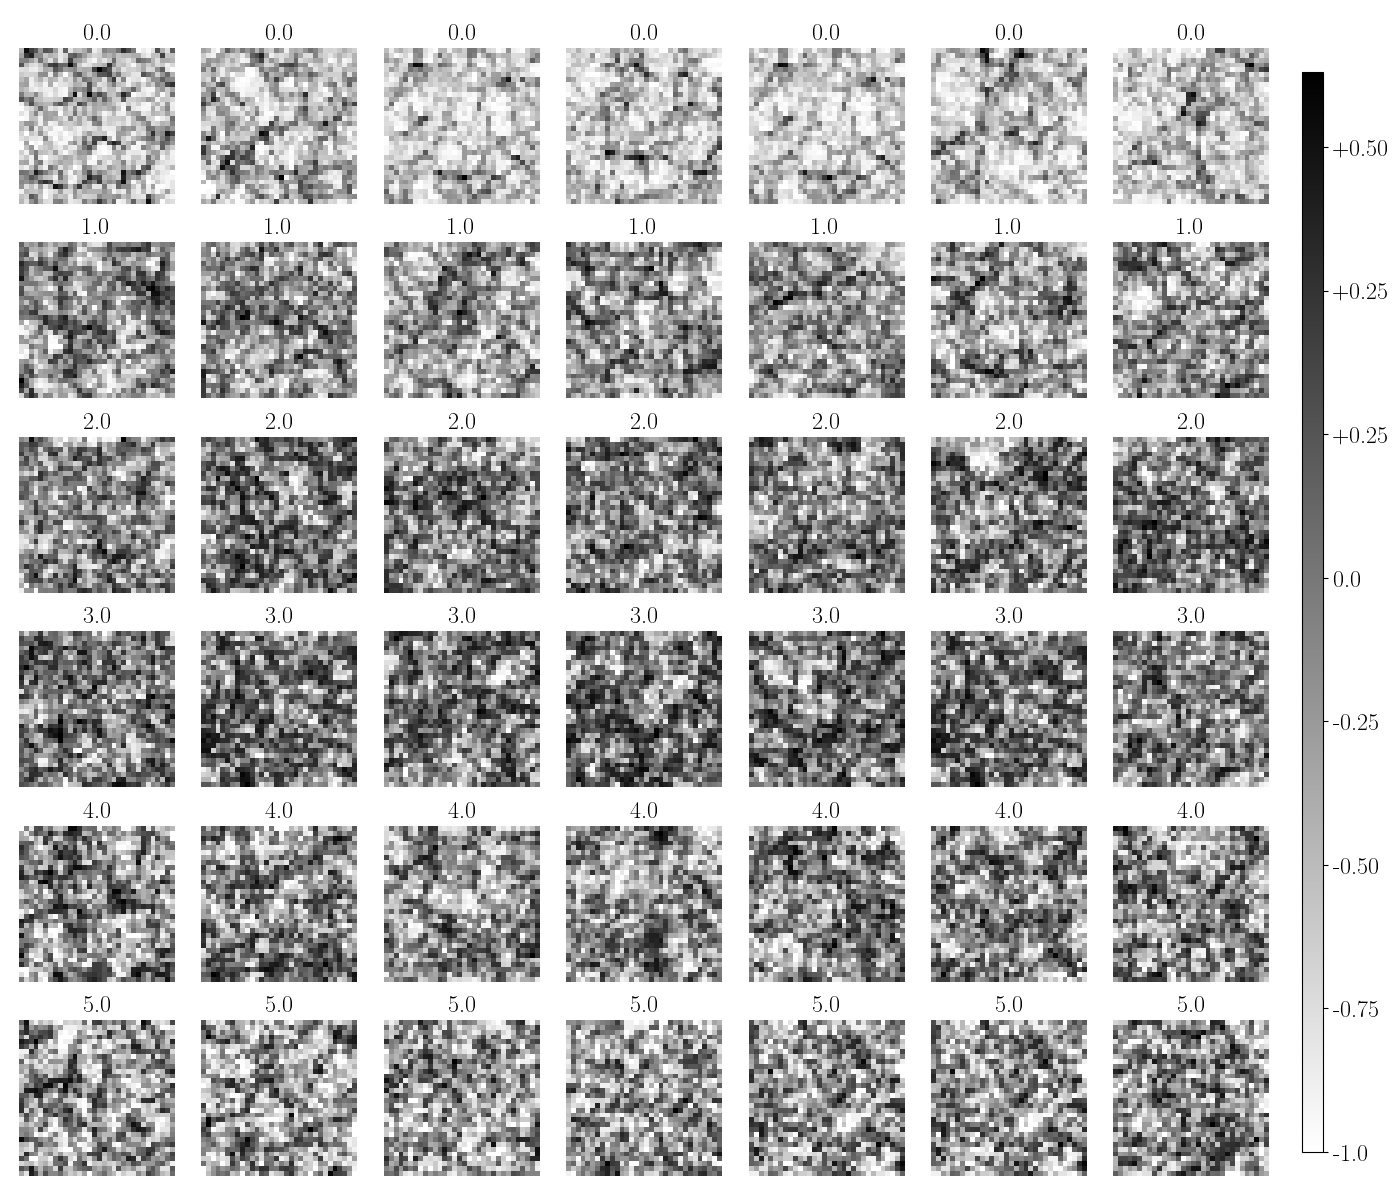
\includegraphics[width=16cm]{figures/cubes/acgan2d_t_fig.png}
% \centering
% \caption{A collection of 2D-projections of training data cubes extracted from the Millennium-SAGE catalogs. Each row 
%          corresponds to the redshift value given above each cube. The scaling $s(\mathbf{x})$ is applied to each cube 
%          $\mathbf{x}$.}
% \label{fig:t_z_imgs_2d}
% \end{figure*}

% \begin{figure*}[hbt!]
% 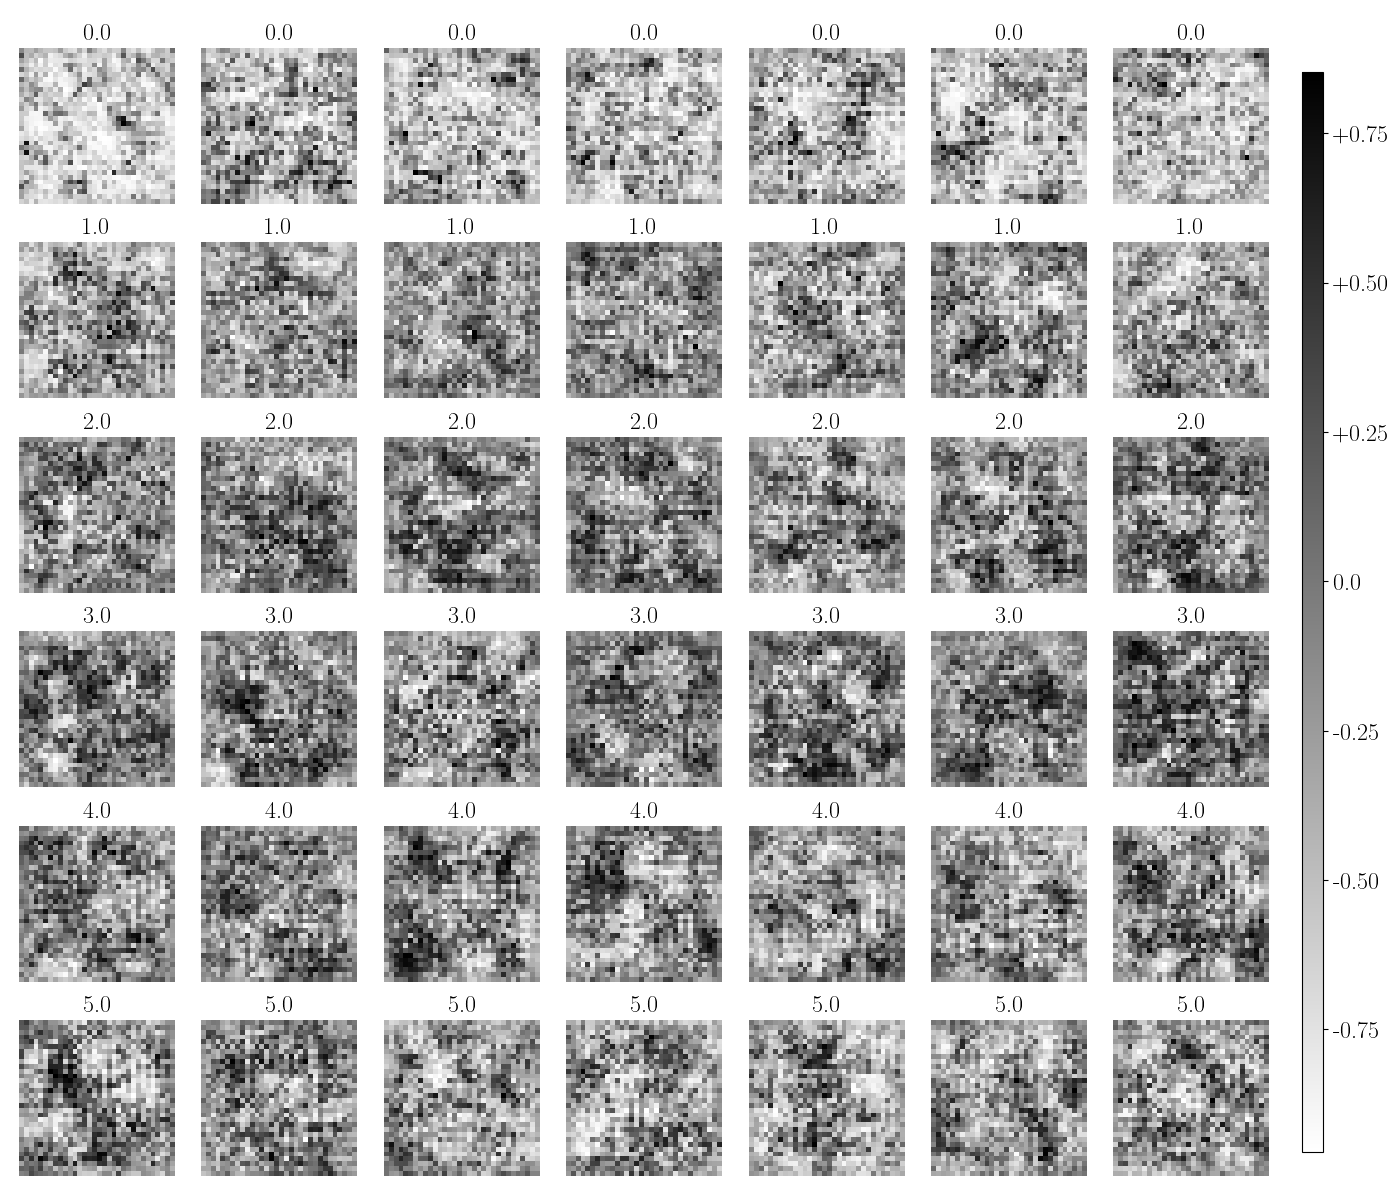
\includegraphics[width=17cm]{figures/cubes/acgan2d_g_fig.png}
% \centering
% \caption{A collection of 2D-projections of generated data cubes extracted from the Millennium-SAGE catalogs. Each row 
%          corresponds to the redshift value given above each cube. The scaling $s(\mathbf{x})$ is applied to each cube 
%          $\mathbf{x}$.}
% \label{fig:t_z_imgs_2d}
% \end{figure*}

%%%%%%%%%%%%%%%%%%%%%%%%%%%%%%%%%%%%%%%%%%%%%%%%%%%%%%%%%%%%%%%%%%%%%%%%%%%%%%%%%%%%%%%%%%%%%%%%%%%%%%%%%%%%%%%%%%%%%%%%%%%

%%%%%%%%%%%%%%%%%%%%%%%%%%%%%%%%%%%%%%%%%%%%%%%%%%%%%%%%%%%%%%%%%%%%%%%%%%%%%%%%%%%%%%%%%%%%%%%%%%%%%%%%%%%%%%%%%%%%%%%%%%%


\subsubsection{Redshift interpolation}
% show grid of cubes ranging from z=0 to z=(highest z in training data classes)

Figure~\ref{fig:acgan_interp} shows the results of varying the class label for a single latent-space point. Between the 
minimum and maximum redshifts $z=0.0$ and $z=5.28$ respectively, 40 class examples were generated. The figure shows a 
smooth evolution of the latent space point evaluated by the generator for redshift $z$. It is left to Section~\ref{sec:kl_trials} 
for a discussion on the validity of the generator samples that are conditioned for $z$ values not in the set of training 
data redshifts, though initial inspection suggests the generator is able to reproduce samples of all redshifts consistently.

\begin{figure}[!ht]%[hbt!]
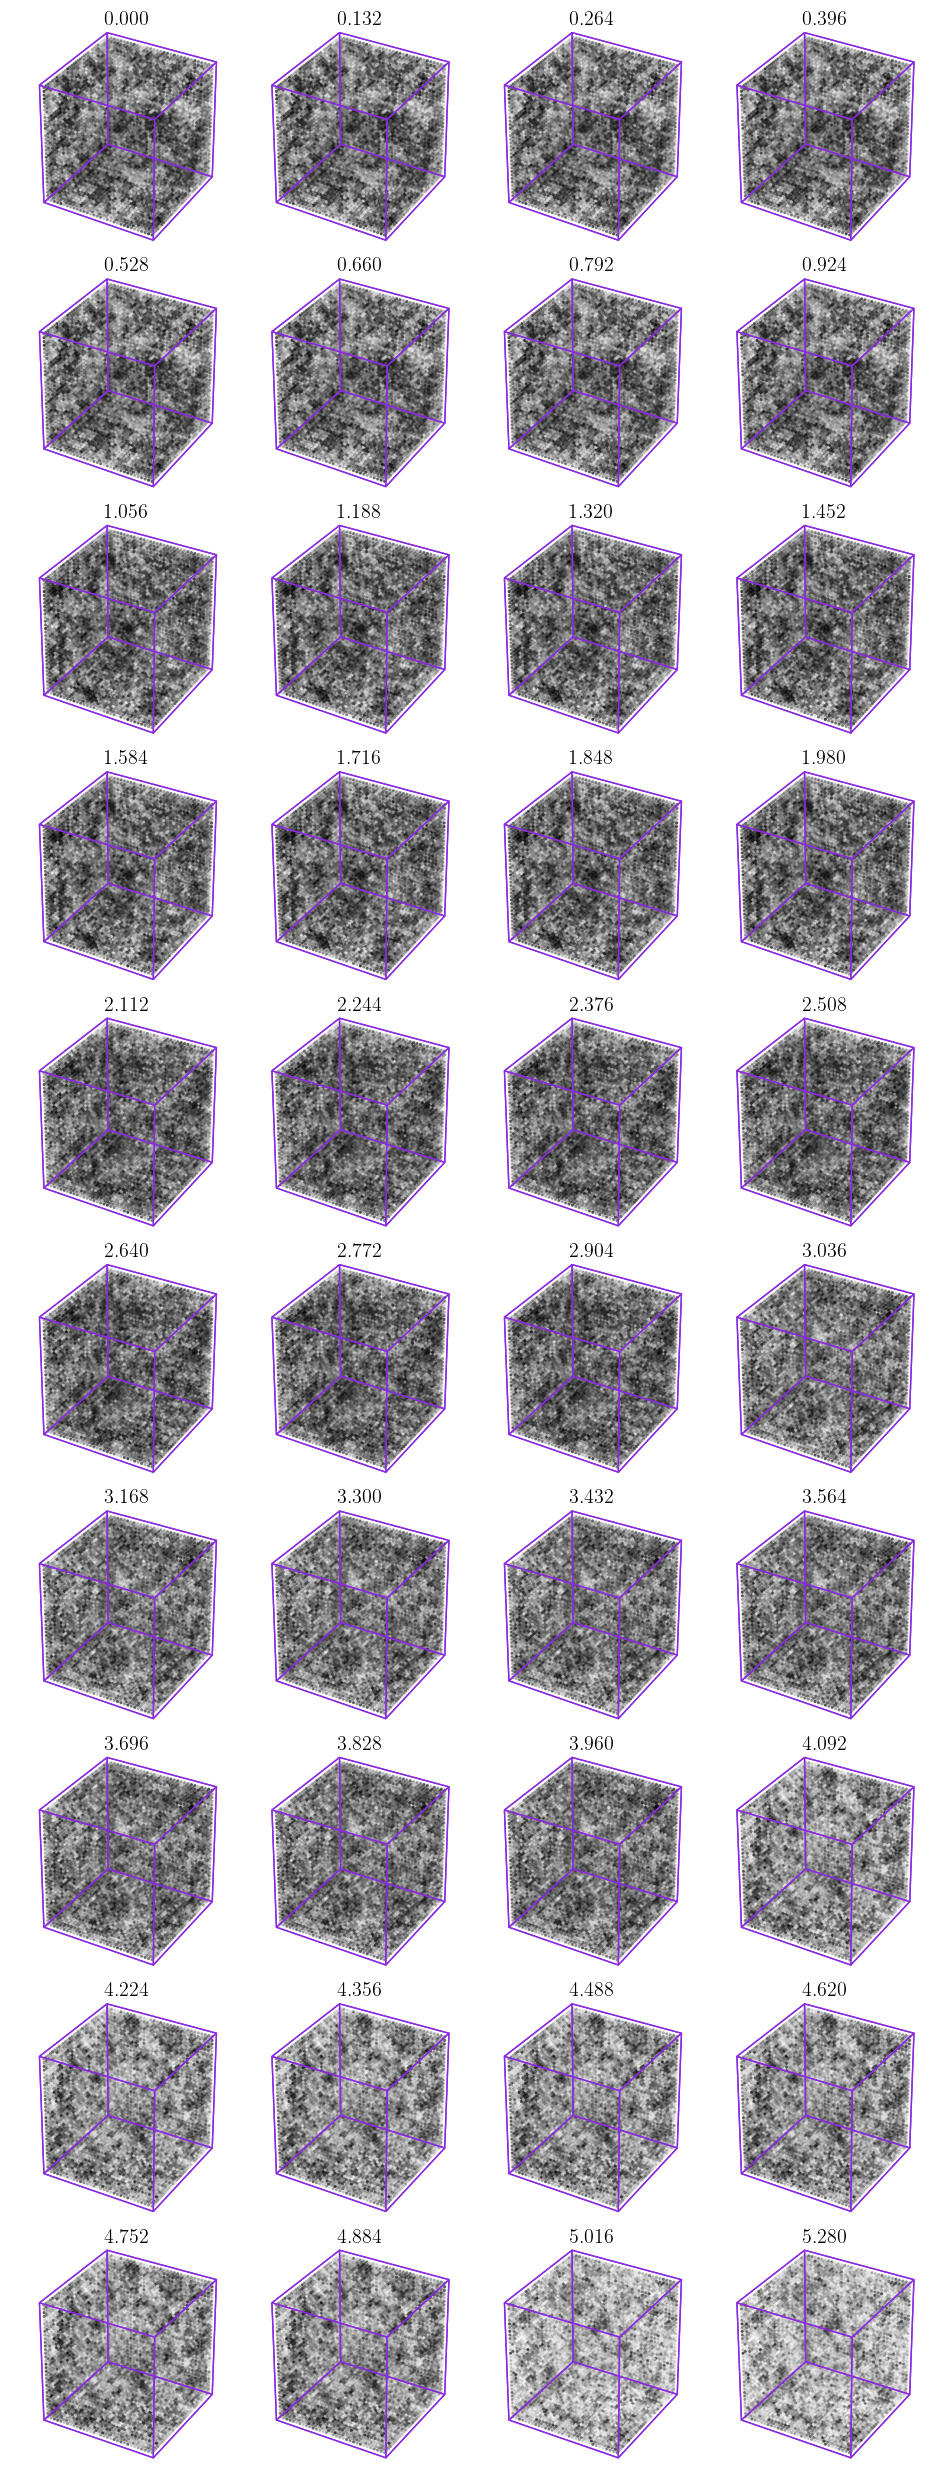
\includegraphics[width=\columnwidth]{figures/cubes/acgan3d_z_spec.png} % acgan3d_interp.png
\centering
\caption{A collection of images generated with an array of redshift values for a single latent-space point.}
\label{fig:acgan_interp}
\end{figure}

% \subsubsection{Universe generation}
% % show three scales (side lengths in terms of generated cubes - e.g. 7, 9, 11) of generated-cube-universes. 

% \begin{figure}[!ht]%[hbt!]
% 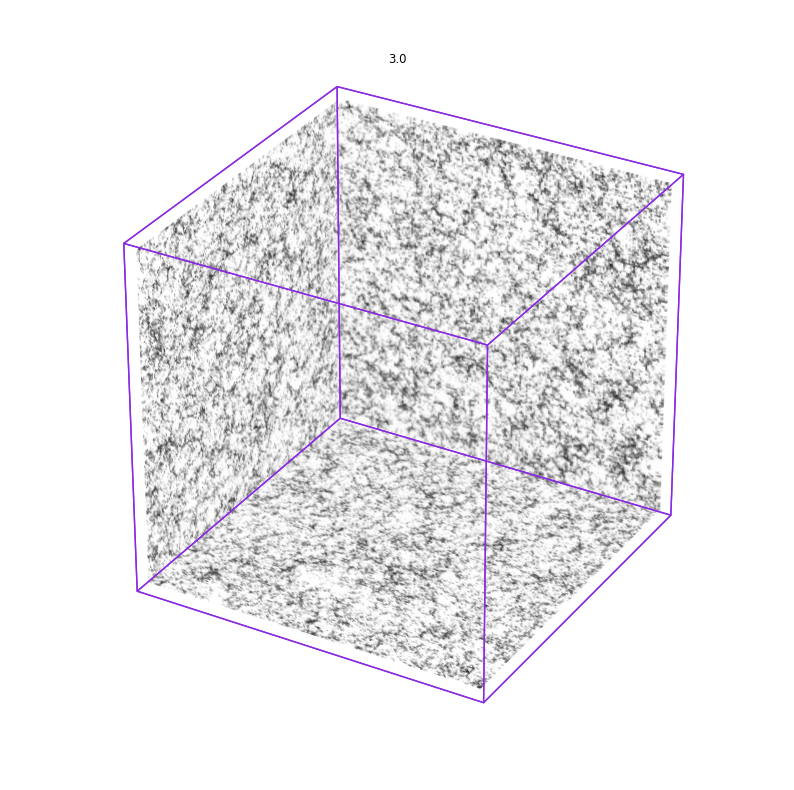
\includegraphics[width=\columnwidth]{figures/cubes/mill_box_3.png}
% \centering
% \caption{A box made of generated cubes at redshift $z=3.19$.}
% \label{fig:kernel_fig}
% \end{figure}

% \begin{figure}[!ht]%[hbt!]
% 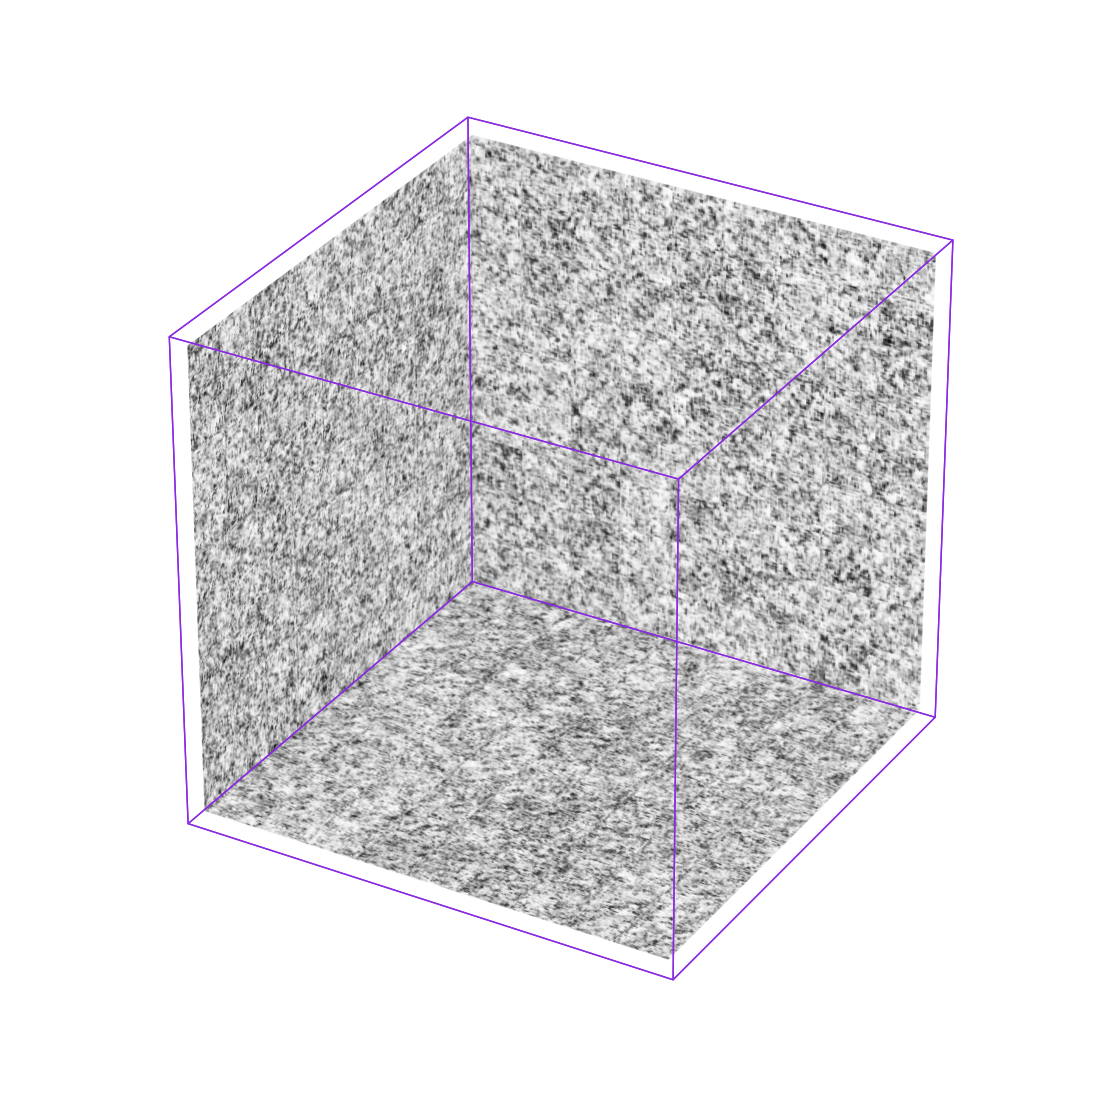
\includegraphics[width=\columnwidth]{figures/cubes/gen_box_9_z3.png}
% \centering
% \caption{A box made of generated cubes at redshift $z=3.00$.}
% \label{fig:kernel_fig}
% \end{figure}

%%%%%%%%%%%%%%%%%%%%%%%%%%%%%%%%%%%%%%%%%%%%%%%%%%%%%%%%%%%%%%%%%%%%%%%%%%%%%%%%%%%%%%%%%%%%%%%%%%%%%%%%%%%%%%%%%%%%%%%%%%%

% \subsubsection{Latent space point interpolation}

%%%%%%%%%%%%%%%%%%%%%%%%%%%%%%%%%%%%%%%%%%%%%%%%%%%%%%%%%%%%%%%%%%%%%%%%%%%%%%%%%%%%%%%%%%%%%%%%%%%%%%%%%%%%%%%%%%%%%%%%%%%

\subsubsection{Unseen redshift testing}
To test the power of the ACGAN generative approach, a selection of redshift values were selected from the Millennium-SAGE
snapshots to obtain new and unseen redshift data. This unseen data was used to register the ability of the generator to
create cubes at a redshift to which the discriminator had never been shown in training. 

The new values of simulation snapshot redshifts are $z'=\{0.51, 1.50, 2.62, 3.58, 4.52\}$ where the original redshift values
$z$ shown to the ACGAN are $z~=~\{0.0, 1.07, 2.07, 3.06, 4.17, 5.28\}$. With these new redshifts the same $D_{KL}$-trials 
were repeated and the results are shown in \ref{fig:kl_trials_all_z2}. A number of similar redshift values to the unseen
redshift values $z'$ are displayed in Figure~\ref{fig:acgan_interp}.
% plot unseen z cubes against true redshifts: 5 rows, 6 cols: 3 real, 3 gen

%%%%%%%%%%%%%%%%%%%%%%%%%%%%%%%%%%%%%%%%%%%%%%%%%%%%%%%%%%%%%%%%%%%%%%%%%%%%%%%%%%%%%%%%%%%%%%%%%%%%%%%%%%%%%%%%%%%%%%%%%%%
%%%%%%%%%%%%%%%%%%%%%%%%%%%%%%%%%%%%%%%%%%%%%%%%%%%%%%%%%%%%%%%%%%%%%%%%%%%%%%%%%%%%%%%%%%%%%%%%%%%%%%%%%%%%%%%%%%%%%%%%%%%

\subsection{Loss curves}
% separation of D and G losses because of number of images shown to models in one training step

% LOSSES AND ACCURACIES
Figure~\ref{fig:acgan_losscurve} shows the ACGAN objectives and accuracies over a run of training. The behaviours of the 
models over the training are apparent in these curves. The initial decline over the first few $10^4$ epochs or so 
shows the initial learning for both models that are new to their tasks. Each sharp jump in the losses of both models shows
the  generator attempting a new strategy for its objective. There are small fluctuations in the accuracies of either model 
as the generator makes smaller adjustments relative to the initial training, just after $1.0\times10^4$ epochs, these are 
in part due to the mistakes made by the discriminator in seeing new training and generated samples. 
% The use of spectral normalisation keeps the weights of the % general

The accuracies and losses of the models in this implementation are extremely chaotic in comparison to typical behaviours of
these parameters in GANs. This is because the spectral normalization regularization constrains the spectral norm of the weight
matrices on each layer it is applied to. This means that changes to this value are always normalised in the next training
iteration. This chaotic behaviour is implicit to the GAN framework and not this implementation itself. The cross entropy loss
is related to the specific KL-divergence we have defined in this work and so the models converging can still be seen in the
$\langle D_{KL}\rangle_z$ curves.

% The accuracies reported by the discriminator model tend very slowly toward around $55\%$. This is an ideal value because the
% discriminator and generator are both engaged in a conflict that still supplies information through gradients to the generator
% model. The samples are still being improved on at this stage. This is echoed in the convergence of the losses for each model 
% to a value of around $9.25$. 
% This does not mean an ideal `perfect' generator has closed the distance between the model and data distributions, but instead 
% that the architecture of the discriminator cannot extract any more useful information (and is extracting less and less) to 
% the generator.The gradients for backpropagation have vanished. This was seen in training. The generator suffered from mode 
% collapse and made more samples with more similarity between them. % NON SN model

% The accuracies of both models converge at just over 60\% which implies there is space to improve the model 
% architectures. The separate networks are not able to fully attain their objectives against each other. At this point the 
% discriminator is extracting the maximal amount of information for use in classification and feedback to the generator, 
% which was observed to be changing the histograms only at the scales given by its convolutional kernels. In other words, 
% the generator is fooling the discriminator without generating the most realistic cubes it could. Through running many 
% different models it was found that $8.0\times 10^4$ epochs was enough time for the network to converge. Past this point 
% the training would dissipate chaotically.

\begin{figure}[!ht]%[hbt!]
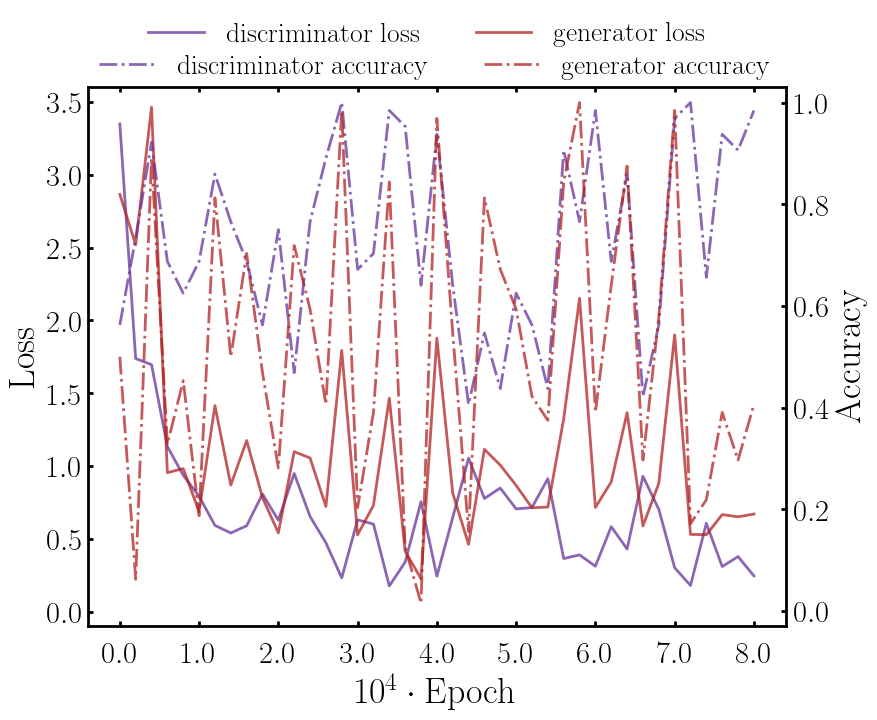
\includegraphics[width=\columnwidth]{figures/graphs/metrics1.png}
\centering
\caption{The loss and accuracy curves for the training of the ACGAN.}
\label{fig:acgan_losscurve}
\end{figure}

\subsection{$D_{KL}$ curves}

The KL divergences between the training and generated distributions $t$ and $g$, denoted by $\langle D_{KL}(t||g) \rangle_z$ 
and $\langle D_{KL}(g||t) \rangle_z$ (where $\langle\dot\rangle_z$ is an averaging over redshift), follow a path that is 
related to the behaviour of the models shown in loss and accuracy curve. The divergences both start at a global maximum and 
tend to a final convergent value. The initial value corresponds to the comparison between batches of cubes with 
pixel-densities sampled from the $\mathbf{z}$-prior $\mathcal{N}(0,1)$ that are devoid of structure and the final value 
corresponds to the cubes with realistic cosmological structure in. 
% The values sharply drop at the same epoch in training as the losses and accuracies do. 
The initial $D_{KL}$ values of the comparison are with earlier generated images that are 
devoid of structure. The final value, with some intermediate values, corresponds to images that are very similar to the 
training data, so the $D_{KL}$ values changed over a range of $10^{1.0}$ to $10^{-1.4}$ from structureless images to 
realistic images.

% The curves have similar features to the loss and accuracy curves as they should because of the relation of the 
% cross-entropy to the KL divergence $D_{KL}$.

The increasingly small differences between the observed $\langle D_{KL}(t||g) \rangle_z$ and $\langle D_{KL}(g||t) \rangle_z$ 
values with respect to the values throughout training is important. This suggests that the training and generated distributions 
$t$ and $g$, and ultimately $p_{model}$ and $p_{data}$ are suited for replacement with each other, as opposed to a preferred 
replacement of one with the other.

\begin{figure}[!ht]%[hbt!]
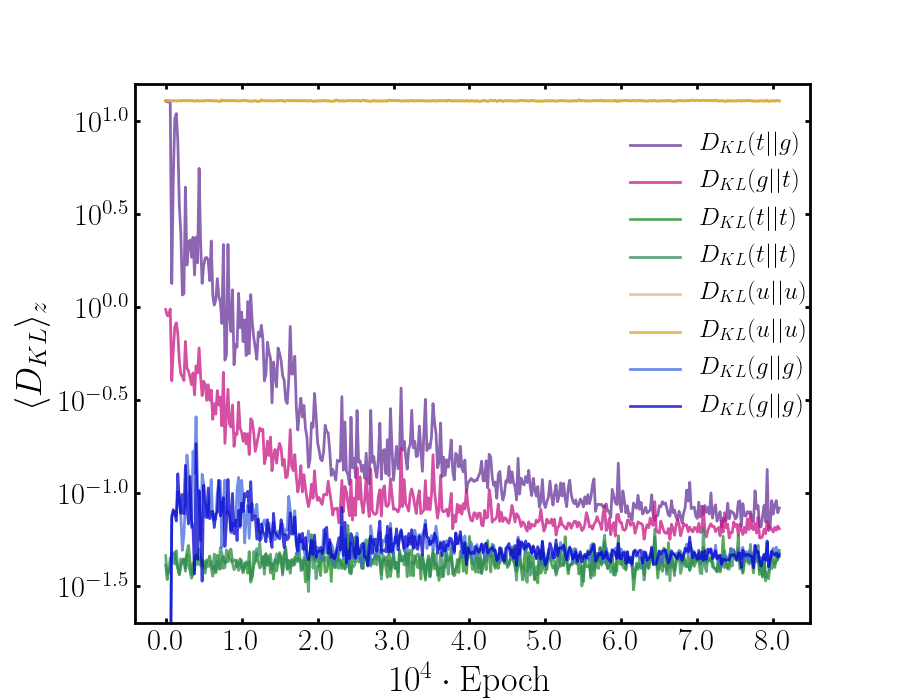
\includegraphics[width=\columnwidth]{figures/graphs/stats1.png}
\centering
\caption{The KL divergence $D_{KL}$ curves for the training of the ACGAN.}
\label{fig:2dgan_losscurve}
\end{figure}

%%%%%%%%%%%%%%%%%%%%%%%%%%%%%%%%%%%%%%%%%%%%%%%%%%%%%%%%%%%%%%%%%%%%%%%%%%%%%%%%%%%%%%%%%%%%%%%%%%%%%%%%%%%%%%%%%%%%%%%%%%%
%%%%%%%%%%%%%%%%%%%%%%%%%%%%%%%%%%%%%%%%%%%%%%%%%%%%%%%%%%%%%%%%%%%%%%%%%%%%%%%%%%%%%%%%%%%%%%%%%%%%%%%%%%%%%%%%%%%%%%%%%%%

\subsection{KL trials}\label{sec:kl_trials}

%%%%%%%%%%%%%%%%%%%%%%%%%%%%%%%%%%%%%%%%%%%%%%%%%%%%%%%%%%%%%%%%%%%%%%%%%%%%%%%%%%%%%%%%%%%%%%%%%%%%%%%%%%%%%%%%%%%%%%%%%%%

\subsubsection{Training redshift trials}

Figure~\ref{fig:kl_trials_all_z1} shows the results of the $D_{KL}$-trials for batches of 64 samples comprised from samples
from each distribution repeated for 128 separate comparisons between each distribution pairing. The procedure for the 
repeated ensemble KL divergence testing outlined in Section~\ref{methods:stats_and_diags} used the samples transformed into 
probability distributions over the pixel density.

There is a slight broadening of the histograms with increasing kernel size. This shows the random effect, or dispersion, 
on the $D_{KL}$ value from repeated tests to on separate ensembles of histograms. This is caused by the loss of information 
due to the down-sampling of larger areas causing more variance in a given value of pixel density because of the averaging 
over the original pixels. This is predicted by the central-limit theorem. In this discussion a `mutual comparison' 
refers to the KL divergence $D_{KL}$ between two different ensembles from the same distribution of $t$, $g$ or $u$. The 
mutual $D_{KL}$ comparisons that show the most broadening are the mutual comparisons which together have increasing 
variance and separation with kernel size. This shows that in both cases the distributions are composed very differently 
to the uniform distributions. The means of the mutual distributions stay the same except for the uniform-uniform comparison. 
This is because the median for the bin separations in the component-histograms was given by the median of the training data 
batch which consistently has a lower mean pixel density than the uniform histogram data. 
% It is also not symmetric as can be seen from the sheer sparsity of the samples for each redshift.


\begin{figure*}[hbt!]
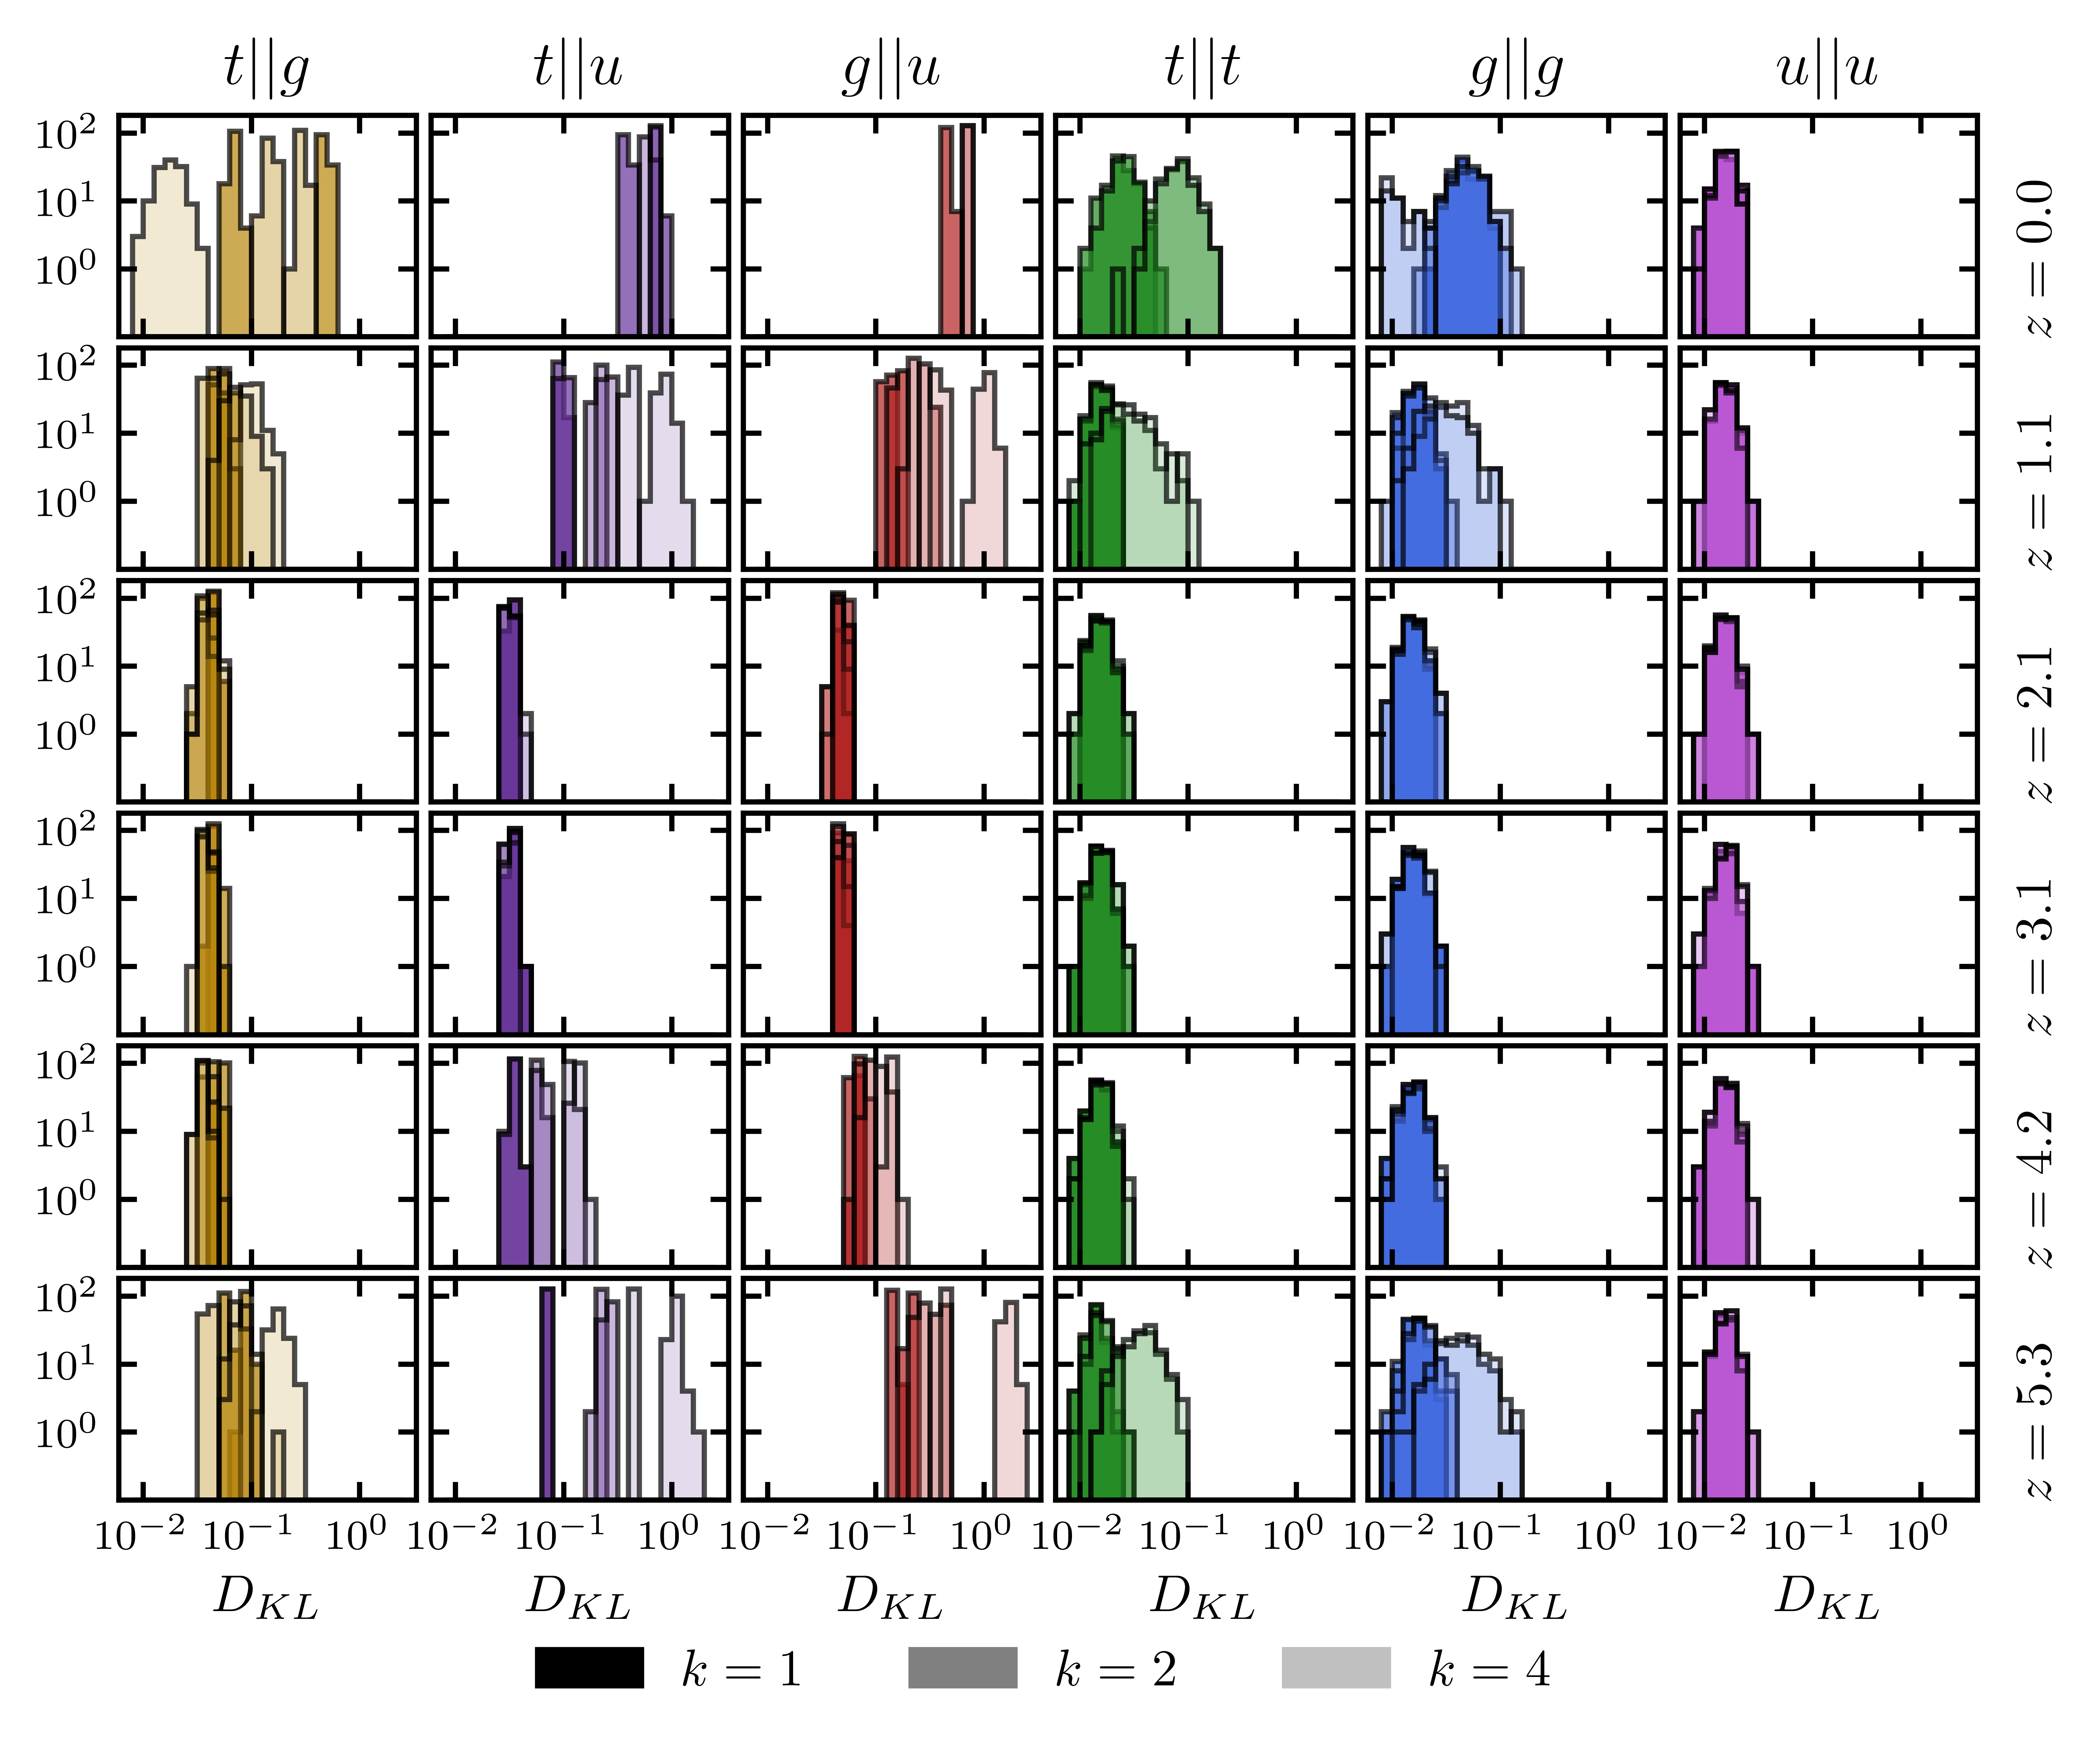
\includegraphics[width=17cm]{figures/graphs/kl_trials_all_z_train1.png}
\centering
\caption{Histograms showing the $D_{KL}$ values for distribution-comparisons between training $t$, generated $g$ and 
         uniform $u$ cube samples. This graph shows the results for downsampling kernel values $k \in \{1, 2, 4\}$.}
\label{fig:kl_trials_all_z1}
\end{figure*}


The similar values of the generated-generated $D_{KL}$ average comparison with the training-training average shows the 
ability of the generator to represent multiple modes in the latent space with as much variety as the simulation data. 
This was affirmed by the training not displaying any mode collapse after converging. The narrower widths of the $t||g$ 
and $g||t$ comparisons stems from the generator creating a subset of images drawn from the data distribution. This could
well be a limitation from the capacity of the model.

The separate kernels cause averaging over different sized volumes. By construction the histograms are already sampling a 
volume at a fixed resolution for every distribution and so the kernel sizes give the same volume at different levels of 
resolution. A histogram from any distribution with each kernel down-sampling will exhibit different scales of structure 
from the original unsampled histogram and this is shown in Figure~\ref{fig:kernel_fig}. The ensembles drawn from each 
distribution are necessary to measure the difference in the structure from the distributions that is not inherent in the 
individual variance of the images themselves. The latter difference does not concern the distributions of the samples and 
is less important for the test of the generator capability. The disparity in the $D_{KL}$ means for each kernel dictates 
how the structure correlates on each scale. The matching alignment of the means along the $t||g$ and $t||t$ columns for 
all values of $k$ provides more evidence for the ability of the generator model. In opposition to this the $t||u$ and $g||u$
columns show $D_{KL}$ means that increase with $k$ and whose separations (between KL comparison means $D_{KL}(a||b)$ and
$D_{KL}(b||a)$) increase.


The widths of the mutual comparison histograms in the $D_{KL}$ trials show that there is an inherent difference in the 
information content of the ensembles from distributions. Some contribution to this is from the difference in the information
content of the batches themselves. Within the fixed specifications of the histograms it would be expected that the mutual 
comparisons show very close values. 

An important characteristic of the training-generated comparisons is that the $D_{KL}$-histograms of these distribution 
pairs overlap. This gives evidence that the distributions can effectively represent each other. The mean $D_{KL}(t||g)$ and 
$D_{KL}(g||t)$ values are all nearly a whole order of magnitude smaller than the training-uniform and generated-uniform 
comparison means. These values of the training-uniform and generated-uniform together show that the generator 
representations are close to the training data because of their similarity in the mean, variance and mean-separations 
for all values of $k$. This shows the generator is able to create samples that are strongly correlated to the training 
data samples, to an extent that is independent of redshift $z$. % check again

% %would liked to have tried to test characteristic statistic of the original dataset

The $D_{KL}$ values of the training-generated comparisons are lower by nearly a whole order of magnitude than the 
training-uniform and generated-uniform comparisons for all kernel sizes. This is the most important result of this report 
because it is evidence for the generator being able to generate samples that are statistically similar to the training data
samples. These values show that much less information would be lost if the model distribution was used in place of the data 
distribution as opposed to the uniform distribution, and that the amount lost is around a factor of two more than that of the 
training distribution approximating itself with different ensembles. This is supported by the horizontal separations of the 
histogram peaks in each column of the first three columns of Figure~\ref{fig:kl_trials_all}. The values of the $D_{KL}(t||g)$ 
and $D_{KL}(g||t)$ are nearly the same as the $D_{KL}(t_1||t_2)$ and $D_{KL}(t_2||t_1)$ values which suggests that replacing 
the $p_{data}$ distribution with the $p_{model}$ distribution would provide realistic samples for the same potential uses 
of the training data. This is because the $D_{KL}(t||t)$ and $D_{KL}(t||t)$ values are nearly the same as the $D_{KL}(t||g)$
and $D_{KL}(g||t)$ values as well as the fact that they are both smaller than the uniform-generated and uniform-training 
comparisons. % check 
The mutual $D_{KL}$ comparisons of the training and generated samples show agreement across the different kernels $k$ and
redshifts $z$. This shows the generators ability to reproduce a variety of structure in the training data samples at a variety 
of redshifts. 
% except for a difference of $10^{-3}$ in the variance of the $k=4$ comparison. 
% The higher $D_{KL}$ average in the $k=1$ training-generated comparisons are expected; the $D_{KL}$ statistic has more individual pieces of information to compare and find differences with. % check exact figures / statements

The $k=4$ kernel, whilst being the largest kernel, does not completely measure the continuity of filament structures over 
a number of the pixels in the $k=4$ down-sampled histograms. This could be tested with a few larger kernel-sizes in histograms 
with a greater number of total pixels. This could also be measured using a cosmological test such as the two-point correlation 
function or power spectrum. An increase in the number of bins for the component-histograms would measure the similarity of
the generator images to the training data images better. The values of the standard deviation of each $D_{KL}$ histogram 
relative to the values of the means suggests the number of trials sufficiently sampled the true $D_{KL}$ mean in each test.
% The empty plot of Figure~\ref{fig:kl_trials_all} appears this way because the density bin boundary is lower than the median 
% and mean of the uniform distribution over the pixel densities. The $D_{KL}$ value for this comparison is much lower than $10^{-2}$.

The differences between the training-uniform and generated-uniform means and variances show the significance of the 
training-generated comparisons. The mean $D_{KL}$ values of the training-generated comparisons are almost at the value of 
the training-training comparison means which is more evidence for the understandings of the training data by the generator. 
The similarity shown by the $D_{KL}(t||g)$ and $D_{KL}(g||t)$ values may mostly be due to the similar pixel density 
distributions of the training and generated data. Considering that the lack of filament structure in the larger scales 
of the generated data compared to the training data is not shown in the $D_{KL}$ comparisons, this may be true. 

The pixel density distribution is an important characteristic of the images but just obtaining the 
similarity between the $t$ and $g$ distributions with this property would not guarantee that all the structure in the 
training data was present. There are many combinations of pixels that make up a matching pixel-density distribution for 
two histogram distributions, but far less of those show the structure of the cosmic web. 
% The higher standard deviations in the $D_{KL}$ histograms for the 2D case in all the kernel sizes compared to the 3D cases is due to the larger size of features relative to total size of the image that shows them in either case.

% \begin{figure*}[hbt!]
% 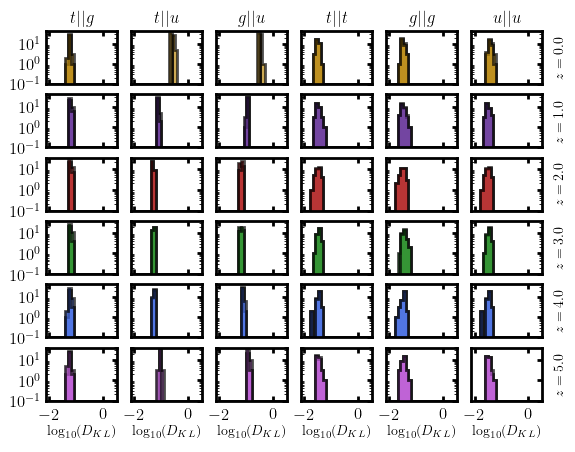
\includegraphics[width=17cm]{figures/graphs/kl_trials_1.png}
% \centering
% \caption{Histograms showing the $D_{KL}$ values for distribution-comparisons between training $t$, generated $g$ and 
%          uniform $u$ cube samples. This graph shows the results for a downsampling kernel of size $k=1$.}
% \label{fig:t_z_imgs}
% \end{figure*}

% \begin{figure*}[hbt!]
% 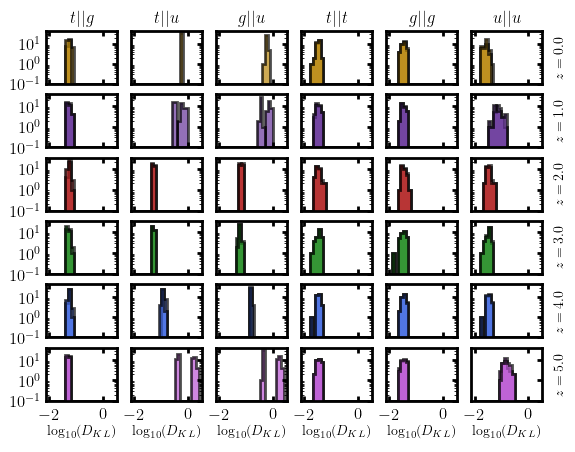
\includegraphics[width=17cm]{figures/graphs/kl_trials_2.png}
% \centering
% \caption{Histograms showing the $D_{KL}$ values for distribution-comparisons between training $t$, generated $g$ and 
%          uniform $u$ cube samples. This graph shows the results for a downsampling kernel of size $k=2$.}
% \label{fig:t_z_imgs}
% \end{figure*}

% \begin{figure*}[hbt!]
% 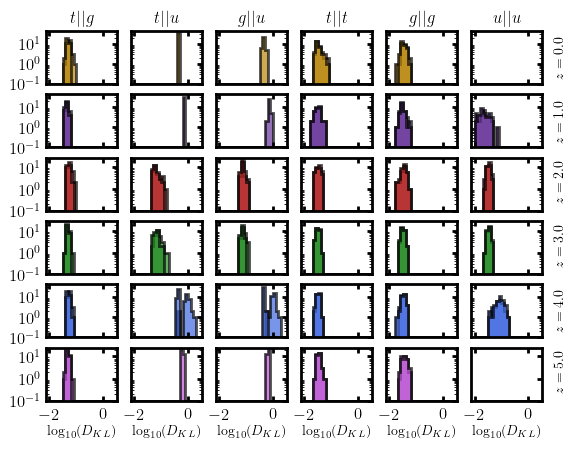
\includegraphics[width=17cm]{figures/graphs/kl_trials_4.png}
% \centering
% \caption{Histograms showing the $D_{KL}$ values for distribution-comparisons between training $t$, generated $g$ and 
%          uniform $u$ cube samples. This graph shows the results for a downsampling kernel of size $k=4$.}
% \label{fig:t_z_imgs}
% \end{figure*}

% \begin{table*}[t]
%   \centering
%   \begin{tabular}{|ccccccc|}
%     \hline\hline
%           & $\langle D_{KL}(t||g) \rangle_z$ & $\langle D_{KL}(t||u) \rangle_z$ & $\langle D_{KL}(g||u)\rangle_z$ & $\langle D_{KL}(t||t)\rangle_z$ & $\langle D_{KL}(g||g) \rangle_z$ & $\langle D_{KL}(u||u) \rangle_z$ \\ 
%           &  $\langle D_{KL}(g||t)\rangle_z$ & $\langle D_{KL}(u||t)\rangle_z$ & $\langle D_{KL}(u||g)\rangle_z$ & $\langle D_{KL}(t||t) \rangle_z$ & $\langle D_{KL}(g||g)\rangle_z$  & $\langle D_{KL}(u||u)\rangle_z$ \\ [1.0ex]
%     \hline\hline
    
%     $k=1$ & $0.060\pm0.005$ & $0.103\pm0.006$ & $0.134\pm0.007$ & $0.032\pm0.006$ & $0.033\pm0.006$ & $0.034\pm0.006$ \\
%           & $0.057\pm0.004$ & $0.088\pm0.005$ & $0.120\pm0.006$ & $0.032\pm0.006$ & $0.033\pm0.006$ & $0.034\pm0.006$ \\ [1ex]

%     $k=2$ & $0.054\pm0.006$ & $2.313\pm0.084$ & $2.317\pm0.165$ & $0.033\pm0.006$ & $0.034\pm0.007$ & $0.059\pm0.016$ \\
%           & $0.052\pm0.005$ & $0.253\pm0.009$ & $0.271\pm0.017$ & $0.033\pm0.006$ & $0.034\pm0.007$ & $0.062\pm0.017$ \\ [1ex]
               
%     $k=4$ & $0.051\pm0.008$ & $6.448\pm0.131$ & $6.492\pm0.418$ & $0.033\pm0.007$ & $0.033\pm0.007$ & $0.030\pm0.009$ \\
%           & $0.049\pm0.006$ & $0.386\pm0.015$ & $0.406\pm0.033$ & $0.033\pm0.007$ & $0.033\pm0.007$ & $0.030\pm0.009$ \\ [1ex]
    
%     \hline\hline
%   \end{tabular}
%   \caption{Results from the $D_{KL}$ trials between each distribution averaged over redshift $z$ for each kernel size $k$.}
%   \label{tab:1}
% \end{table*}

%%%%%%%%%%%%%%%%%%%%%%%%%%%%%%%%%%%%%%%%%%%%%%%%%%%%%%%%%%%%%%%%%%%%%%%%%%%%%%%%%%%%%%%%%%%%%%%%%%%%%%%%%%%%%%%%%%%%%%%%%%%

\subsubsection{Unseen redshift trials}

Figure~\ref{fig:kl_trials_all_z2} shows the results of the $D_{KL}$-trials between for batches of 64 
samples from each distribution repeated for 128 separate comparisons between each distribution pairing. These results are 
produced by using the generator to create samples at values of redshift $z=z'$ that the ACGAN has never been exposed to.

\begin{figure*}[hbt!]
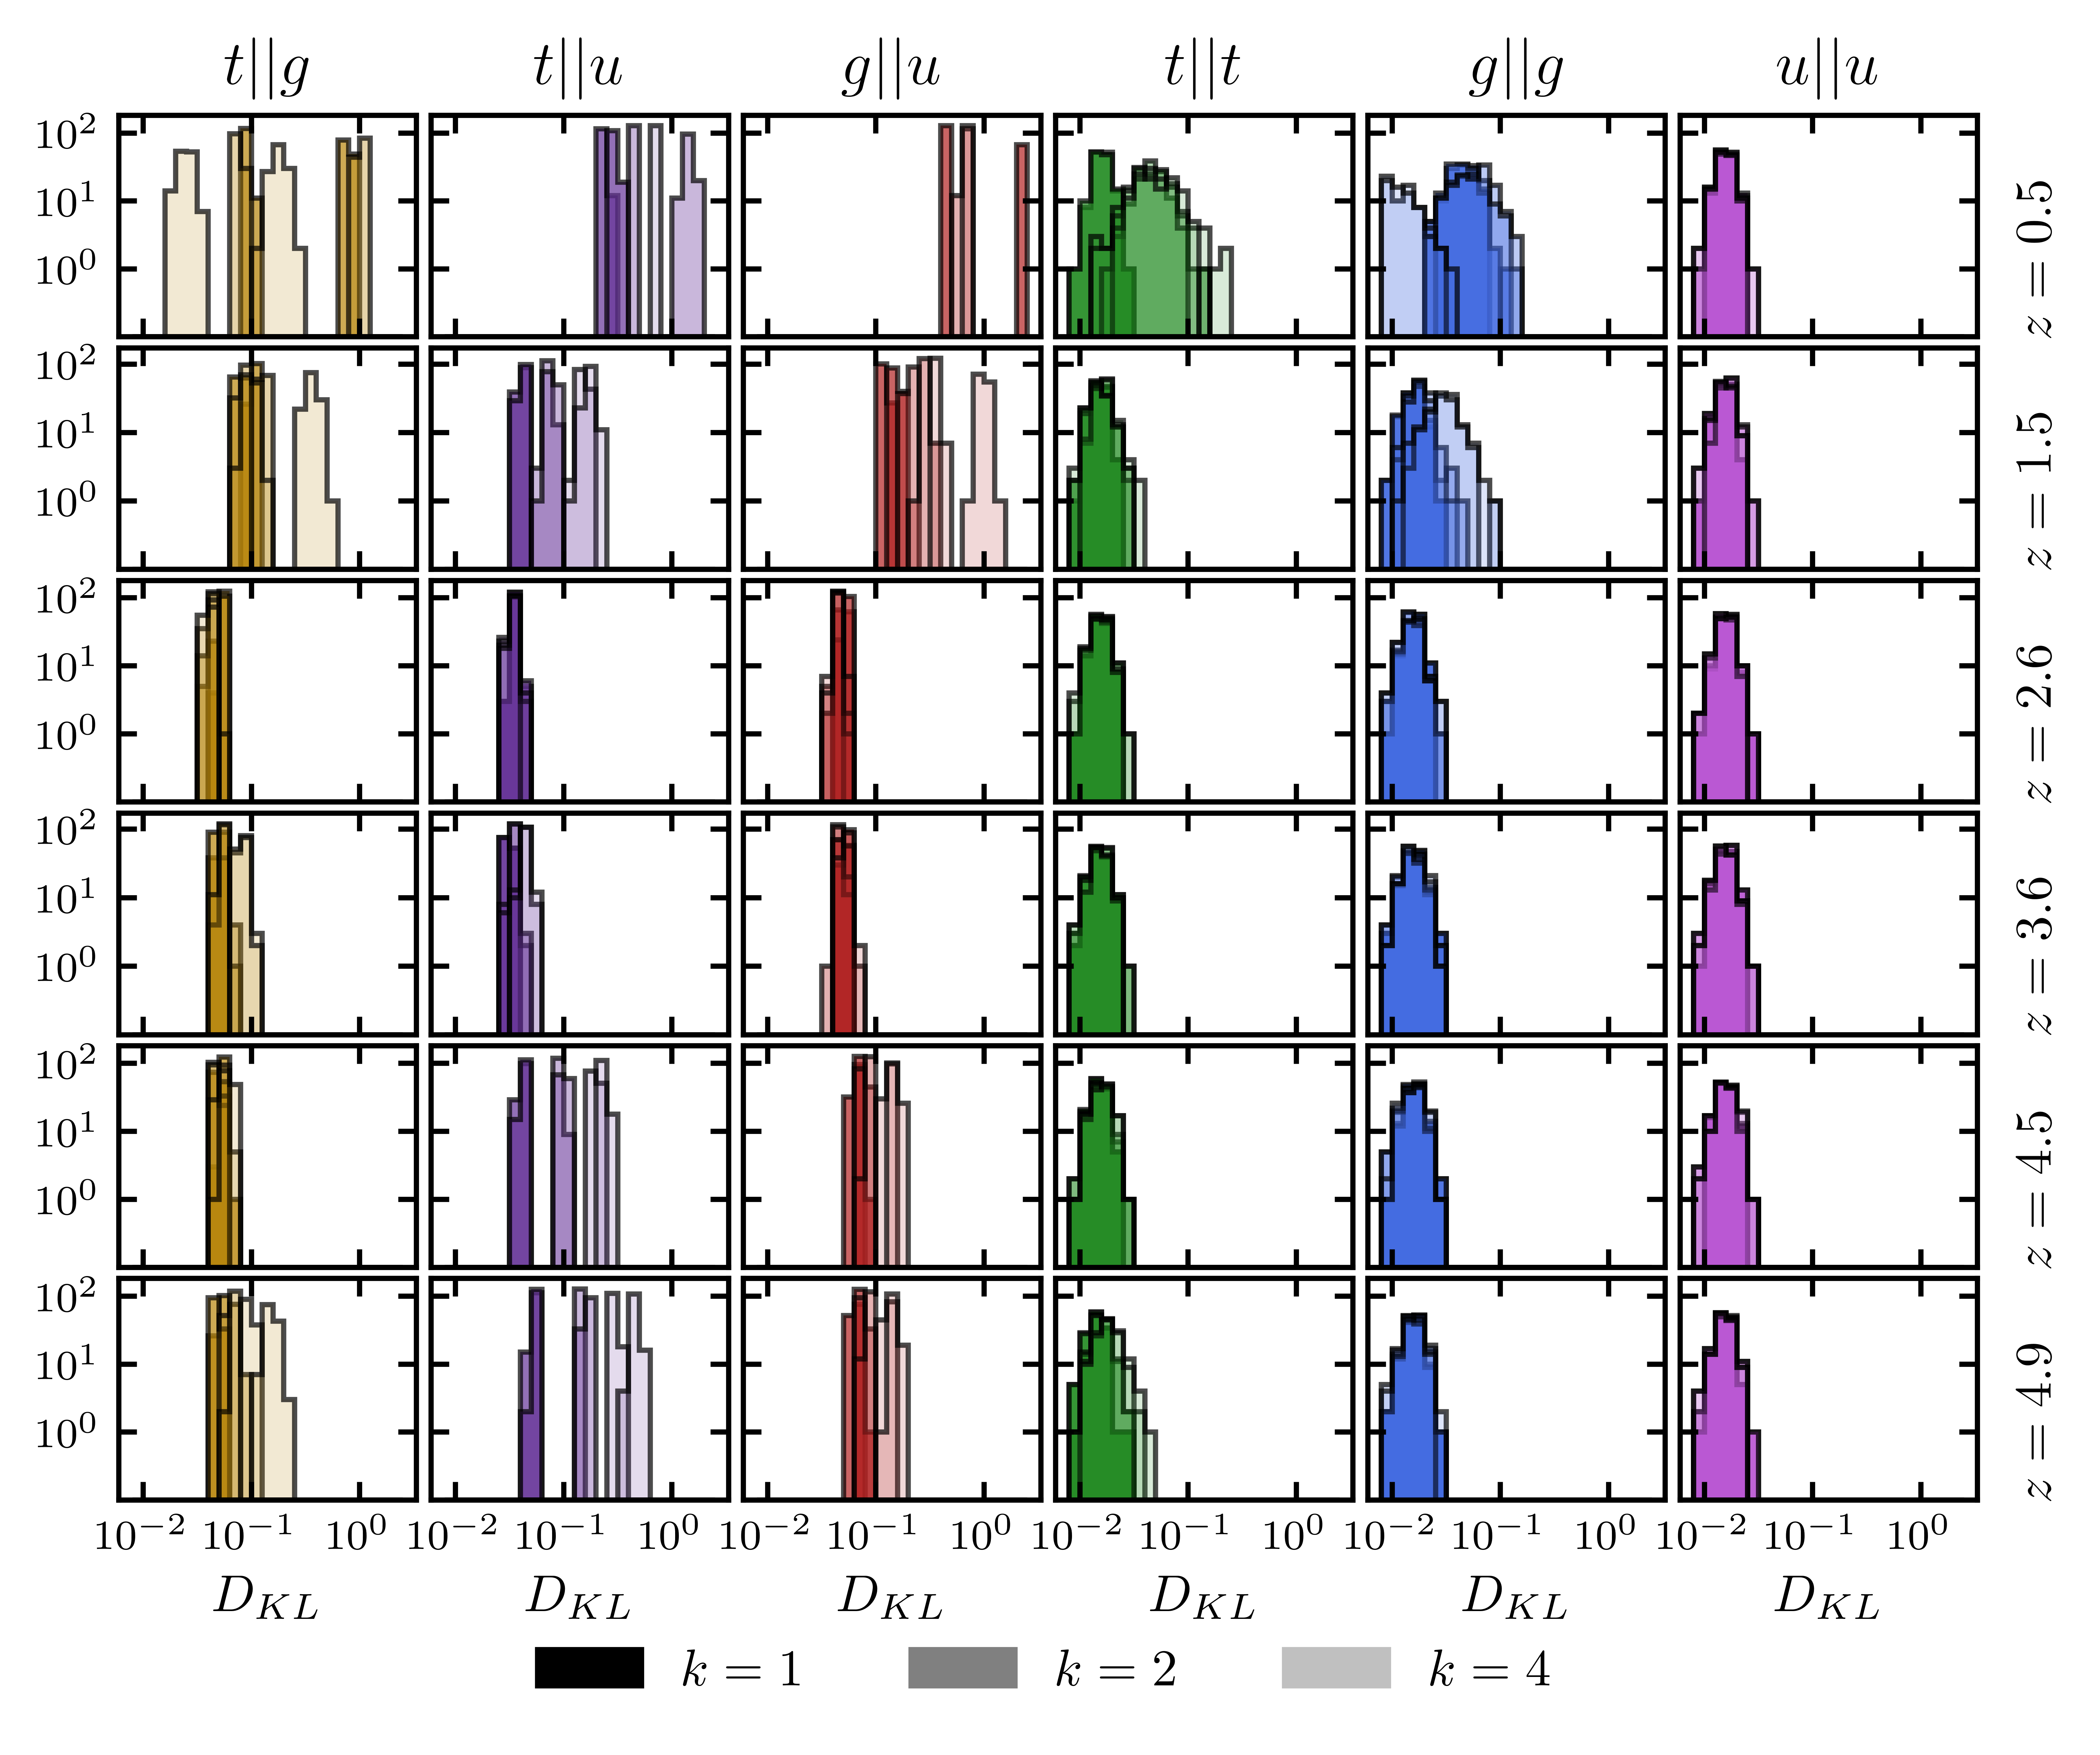
\includegraphics[width=17cm]{figures/graphs/kl_trials_all_z_unseen1.png}
\centering
\caption{Histograms showing the $D_{KL}$ values for distribution-comparisons between training $t$, generated $g$ and 
         uniform $u$ cube samples with cube samples from unseen redshift snapshots in the Millennium-SAGE simulation 
         data This graph shows the results for downsampling kernel values $k \in \{1, 2, 4\}$.}
\label{fig:kl_trials_all_z2}
\end{figure*}

% \begin{table*}[t]
%   \centering
%   \begin{tabular}{|ccccccc|}
%     \hline\hline
%           & $\langle D_{KL}(t||g) \rangle_{z'}$ & $\langle D_{KL}(t||u) \rangle_{z'}$ & $\langle D_{KL}(g||u)\rangle_{z'}$ & $\langle D_{KL}(t||t)\rangle_{z'}$ & $\langle D_{KL}(g||g) \rangle_{z'}$ & $\langle D_{KL}(u||u) \rangle_{z'}$ \\ 
%           &  $\langle D_{KL}(g||t)\rangle_{z'}$ & $\langle D_{KL}(u||t)\rangle_{z'}$ & $\langle D_{KL}(u||g)\rangle_{z'}$ & $\langle D_{KL}(t||t) \rangle_{z'}$ & $\langle D_{KL}(g||g)\rangle_{z'}$  & $\langle D_{KL}(u||u)\rangle_{z'}$ \\ [1.0ex]
%     \hline\hline
    
%     $k=1$ & $0.146\pm0.010$ & $0.100\pm0.005$ & $0.073\pm0.005$ & $0.069\pm0.004$ & $0.081\pm0.004$ & $0.109\pm0.007$ \\
%           & $0.033\pm0.006$ & $0.033\pm0.006$ & $0.036\pm0.007$ & $0.036\pm0.007$ & $0.033\pm0.006$ & $0.033\pm0.006$ \\
%           [1ex]
    
%     $k=2$ & $0.650\pm0.045$ & $0.166\pm0.007$ & $1.390\pm0.074$ & $0.208\pm0.009$ & $0.343\pm0.021$ & $0.174\pm0.011$ \\
%           & $0.033\pm0.006$ & $0.033\pm0.006$ & $0.059\pm0.013$ & $0.061\pm0.014$ & $0.067\pm0.014$ & $0.067\pm0.014$ \\
%           [1ex]
               
%     $k=4$ & $2.233\pm0.120$ & $0.253\pm0.011$ & $5.658\pm0.358$ & $0.417\pm0.022$ & $2.986\pm0.249$ & $0.353\pm0.025$ \\
%           & $0.033\pm0.008$ & $0.032\pm0.008$ & $0.061\pm0.018$ & $0.062\pm0.017$ & $0.080\pm0.025$ & $0.080\pm0.025$ \\
%           [1ex]
%     \hline\hline
%   \end{tabular}
%   \caption{Results from the $D_{KL}$ trials between each distribution averaged over values of unseen redshift $z'$ for each 
%           kernel size $k$.}
%   \label{tab:2}
% \end{table*}

The results point to the fact that the generator is competent at representing values of redshift that lay between the
values that the ACGAN has been exposed to in training. This is interesting because the description for the emergence
of the finite training set of images is certainly more simple than the chronology of the cosmic web that the Millenium-SAGE
models characterise. Figure~\ref{fig:z_kl} shows the relation between the $\langle D_{KL}(g||t) \rangle$ and 
$\langle D_{KL}(t||g) \rangle$ values with redshift $z$. The highest peak coincides with the lowest unseen redshift $z'=0.51$.

The last two unseen redshift values show consistency between kernel sizes and they are similar values to the trained redshift 
values either side of these redshifts. Because these $\langle D_{KL} \rangle$ values have the lowest separation between the 
nearest trained redshifts, it suggests that the ACGAN has trouble obtaining the same coherence in samples either side of the 
median $z$ value of the data it is exposed to. The coherence of the $z$ redshift samples to the $z'$ redshift samples suggests
the ACGAN can represent samples to a distance away from a given trained redshift value of between 0.3 and 0.5.

The similarity between the lowest and highest $z$ and $z'$ $D_{KL}$-histograms suggests that the characteristics of the data 
cause the ACGAN some difficulty in imitating samples at these redshifts successfully, but that it is not necessarily a deficiency 
that only this implementation of the ACGAN would suffer with.

% lack of data? lack of feature maps

\begin{figure}[!ht]%[hbt!]
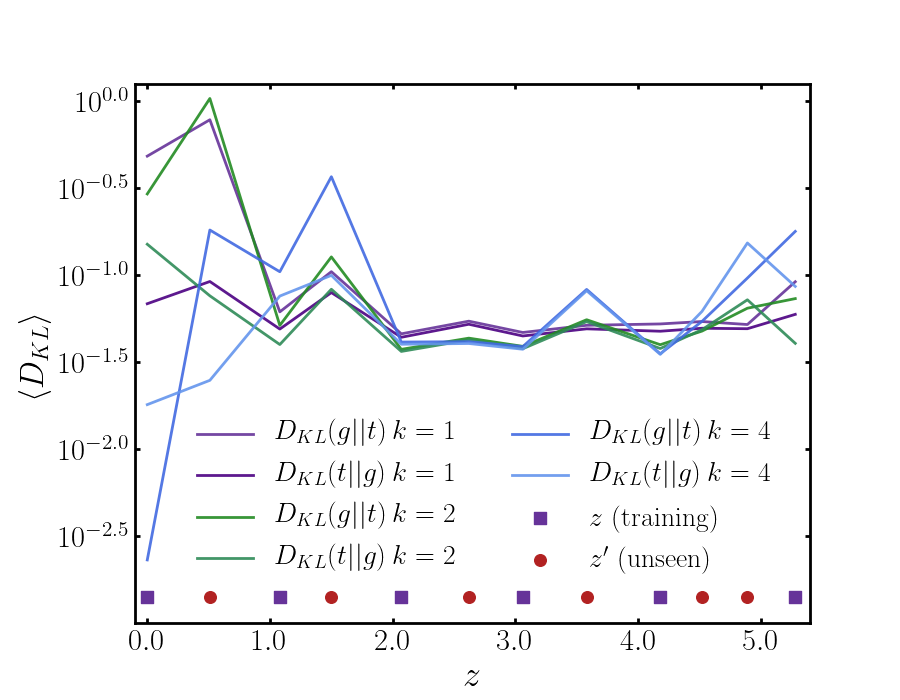
\includegraphics[width=\columnwidth]{figures/graphs/z_kl4.png}
\centering
\caption{The KL-trial means $\langle D_{KL} \rangle$ for comparisons of image distributions 
         $t$ and $g$ for all redshifts $z$ and $z'$ }
\label{fig:z_kl}
\end{figure}



%%%%%%%%%%%%%%%%%%%%%%%%%%%%%%%%%%%%%%%%%%%%%%%%%%%%%%%%%%%%%%%%%%%%%%%%%%%%%%%%%%%%%%%%%%%%%%%%%%%%%%%%%%%%%%%%%%%%%%%%%%%
%%%%%%%%%%%%%%%%%%%%%%%%%%%%%%%%%%%%%%%%%%%%%%%%%%%%%%%%%%%%%%%%%%%%%%%%%%%%%%%%%%%%%%%%%%%%%%%%%%%%%%%%%%%%%%%%%%%%%%%%%%%
%%%%%%%%%%%%%%%%%%%%%%%%%%%%%%%%%%%%%%%%%%%%%%%%%%%%%%%%%%%%%%%%%%%%%%%%%%%%%%%%%%%%%%%%%%%%%%%%%%%%%%%%%%%%%%%%%%%%%%%%%%%

\section{Future work}\label{sec:future_work}
% HPC resources on GANs 
At this outset the capability to generate independent 3D galaxy distributions is the beginning of the full application of 
generative modelling in teaching a machine to generate an artificial universe. The proceeding sections will show potential 
research into achieving the full objective.

%%%%%%%%%%%%%%%%%%%%%%%%%%%%%%%%%%%%%%%%%%%%%%%%%%%%%%%%%%%%%%%%%%%%%%%%%%%%%%%%%%%%%%%%%%%%%%%%%%%%%%%%%%%%%%%%%%%%%%%%%%%
%%%%%%%%%%%%%%%%%%%%%%%%%%%%%%%%%%%%%%%%%%%%%%%%%%%%%%%%%%%%%%%%%%%%%%%%%%%%%%%%%%%%%%%%%%%%%%%%%%%%%%%%%%%%%%%%%%%%%%%%%%%

\subsection{Improvements to the present method}
The strongest dependence of the quality and realism of the generator product are the GAN models and hyper-parameters. It 
should be noted that each of these should really be tested independently but it is quite possible that a lifetime is not 
long enough to do so. The author's opinion is that the best route is to improve the current architecture by increasing the 
number of pixels in the cubes, allowing the depth of the models to increase with more layers, whilst also better translating
the variance in the structure inside the histograms. It has been found that in amplifying the initial parameterised units 
in the first layer of the generator model requires that there are at least $\sim \! 10^4$ units. The use of
fewer units does not allow the generator to draw enough permutations from the potential `proto-cubes' allowed by the 
initial layer. The kernels in the convolutional layers were found to be most effective at size $9 \times 9 \times 9$. 
Though it is expected that some combination of higher kernel sizes would better characterise the histogram structures. 

A larger original simulation with which to sample training data would help the networks process differences between 
individual samples. The larger volume would give more homogeneous samples with less variance in the summary statistics 
per sample. 
% The means, total densities and variances of the pixel distributions in each cube were calculated in each 
% iteration of training. Monitoring these statistics showed that the their variance was up to 10\% of their total values 
% each. Increasing the homogeneity of the samples would decrease this value. 
The sizes of the samples relative to the original simulation volume could also be increased from the tested value to
increase the homogeneity of the samples. Increasing the sample cube size would also allow the $D_{KL}$ testing to consider
more varied structure in the kernel sizes. 

% The $D_{KL}$ trials could be repeated to compare the 3D two-dimensional cube projections with the 2D generated images 
% and training data. This would connect the results of the separate 2D and 3D implementations. For both of the 
% implementations the $p_{KS}$ testing could have been repeated in the same way as the $D_{KL}$ tests to give more 
% understanding of the differences between the distributions. In this work the $p_{KS}$-values would be better understood
% if they were compared to other distribution comparison $p_{KS}$-values.

The other available galaxy properties from the Millennium-SAGE catalogs could also be folded into the generator analysis
to create distributions weighted by luminosity or another characteristic. It is possible that some amount of control over
the generated images and their additional characteristics could deepen the effectiveness of replacing simulation data in 
analyses, allowing samples that are emergent from different cosmological parameters to be considered separately.

In previous work, a regular GAN was trained on the same $z=0$ data and a smaller difference in the mean $D_{KL}(t||g)$ value
was found. As a one class model, this suggests that the architectures in this ACGAN implementation could require a higher 
capacity in terms of convolution filters. The differences in the pixel sparsity between redshift classes increases the need
for more filters in the ACGAN convolutions.
% 3D model works REALLY well - use transposed conv instead of upsampling. As a one-class model, the capacity implies that the
% ACGAN requires more filters that the GPU could not provide.

%%%%%%%%%%%%%%%%%%%%%%%%%%%%%%%%%%%%%%%%%%%%%%%%%%%%%%%%%%%%%%%%%%%%%%%%%%%%%%%%%%%%%%%%%%%%%%%%%%%%%%%%%%%%%%%%%%%%%%%%%%%
%%%%%%%%%%%%%%%%%%%%%%%%%%%%%%%%%%%%%%%%%%%%%%%%%%%%%%%%%%%%%%%%%%%%%%%%%%%%%%%%%%%%%%%%%%%%%%%%%%%%%%%%%%%%%%%%%%%%%%%%%%%

\subsection{Redshift and structure interpolation} 
The latent space from which the generator model samples noise-vectors to change into samples from the model distribution 
encodes informative features in the natural data samples. This latent space can be navigated, typically along the separate 
axes, to interpolate through the features. This could be implemented in the latent space of an ACGAN that is trained on 
data with different redshifts to interpolate between different values of redshift in an inexpensive procedure. This 
interpolation may hold the ability to evolve a collection of samples simultaneously by interpolating through redshift 
values in a continuous way. 

% In the research for this publication, arrays of samples generated by points constituting a path in the latent-space. Uniform
% (along collinear points on one axis) and Gaussian interpolation along a hypershere

% \subsubsection{Latent space navigation}\label{methods:z_navig}
% % show the maths behind it, the general method of doing it. See https://arxiv.org/pdf/1609.04468.pdf, % (Larsen et al., 2016).
In all non-trivial cases, the number of parameters available to the generative model of a GAN through its architecture is 
less than the total parameters that constitute the training set. This means the discriminator and generator must find 
condensed representations of the training data. The generator model is sampled from a set of latent variables in the 
latent space that constitute the latent-vectors $\mathbf{z}$. Vector space arithmetic with points in the latent space 
allows interpolation between tenable examples of learned representations of the training data the GAN is exposed to in 
training. 
% % With the inherent structuring of the latent space by GANs, these operations can allow complex 

Interpolation is the transit between two distinct points in the latent space. In research for this work, spherical interpolation 
was tested as opposed to linear interpolation. The latter being a over-simplistic approach as the latent space of the model 
trained in this work had 256 dimensions with a Gaussian prior $\mathcal{N}(0,1)$. Spherical interpolation~\cite{spherical_interp} uses a great circle arc on the N-dimensional hypersphere in the latent space, with a path given by 

\begin{equation}
    S(q_1, q_2; \mathbf{\mu}) = \frac{\sin (1 - \mu)\theta}{\sin \theta}q_1 + \frac{\sin \mu\theta}{\sin \theta}q_2
\end{equation}

where a discrete set of points between points $q_1$ and $q_2$ are passed to the generator model to create samples~with and
$\mu$ are the discrete proportioned steps between $q_1$ and $q_2$. It should be noted that simple linear interpolation 
along a given axis of the latent space would disregard the curvature of the 256-dimensional latent space and so the path 
along a great circle by spherical interpolation is required.

Typical applications of generating samples along paths interpolated as above concern representations of more natural images.
This type of data, being more tangible to humans, permits results of vector arithmetic in the latent space to be judged easily.
With samples of the cosmic web no such comparisons can be so easily made - it remains a target of future work to explore the 
potential of isolating regions in the latent space according to physically-semantic features in the samples produced using points
there. It is potentially possible to characterise samples in the latent space to query the generator for samples that display, for
example, more or less filament structure. 

%% In these cases, we have performed a linear interpolation which assumes that the latent space is uniformly distributed 
%% hypercube. Technically, our chosen latent space is a 100-dimension hypersphere or multimodal Gaussian distribution.

The problem of mode collapse for the generator model could be estimated by interpolating the 
latent space to create a sample of images to test with each other for similarity. A simple test would be to create the 
mean-image of this sample to test for overlaps but more advanced cross-correlations could show more detail of the overlaps.  

%%%%%%%%%%%%%%%%%%%%%%%%%%%%%%%%%%%%%%%%%%%%%%%%%%%%%%%%%%%%%%%%%%%%%%%%%%%%%%%%%%%%%%%%%%%%%%%%%%%%%%%%%%%%%%%%%%%%%%%%%%%
%%%%%%%%%%%%%%%%%%%%%%%%%%%%%%%%%%%%%%%%%%%%%%%%%%%%%%%%%%%%%%%%%%%%%%%%%%%%%%%%%%%%%%%%%%%%%%%%%%%%%%%%%%%%%%%%%%%%%%%%%%%

\subsection{Universe generation} 
To create a cosmological volume on order of the size of the Millennium-SAGE volume, with the tested default cube-size, a 
generator would need to create around $20$ cubes. The generator model in this work once trained can do so within 
seconds. Whilst in the process of fusing the samples together coherently avoiding density discontinuities would not be a 
trivial task, it is logical to assume that it is a process that is maximally as intensive as generating the cubes 
themselves. It is expected that the GAN would be able to generalise well to higher resolution or larger volume sample data.  

The scaled volumes produced by the GAN require the value of the total number of galaxies contained in the cubes to 
transform the cubes back into coordinate tensors - the initial objects extracted from the simulation. This would be done 
by uniformly distributing the number of galaxy positions required for each histogram cell into each cell. The value of the
total number of galaxies can be passed to the GAN framework and detached to a separate `route' in the models. This value, 
like the histogram cells, would be correctly posited just as the histogram pixel densities are in training. An important 
test for the methods presented would be to compare the original simulation coordinate tensors to those built from generated
samples. 

% Find a way to co-interpolate a massive volume of cubes between different redshifts


% \subsection{Generative variants}
% Some of the other possible architectures and variants of the GAN framework could be implemented to see if there 
% was a efficient or more successful model for the objective in this report. A Wasserstein Generative Adversarial Network
% (WGAN)~\cite{wgan} was tested but it was not found to work as well as the original GAN. The Wasserstein loss function 
% cannot be extended to a categorical version for use in a conditional GAN so if different redshift samples are required 
% for an application the WGAN method would not work anyway. 

% \subsection{Parallelised GANs} 
% One of the problems of training GANs is being sure that the most profitable convergence, best performing 
% architectures and greatest accuracies are obtained. If further work is able to prove that the use of generative models
% can mimic cosmological structure with enough variety and realism, then the High Performance Computing (HPC) resources 
% used for simulations could be used for creating even larger and more detailed cosmological simulations. The concept has
% been shown to work for smaller datasets and generative models in~\cite{parallel_gan1, parallel_gan2}. This is particularly
% important for the case of cosmological simulations because previous simulations involve using assumptions such as the 
% Zel'dovich Approximations~\cite{zeld_approx} and complex numerical codes~\cite{FPM, gadget2}. Deep learning models are 
% not limited to using low order representations for structural phenomena such as clustering~\cite{lagrangian_approx}. The
% datasets available to parallelised generative models can also be far larger and with HPC resources they can use deeper 
% models to process structure at higher resolution. 

% % The ideal, computationally intractable, way to train a GAN to achieve the most statistically sound convergence of 
% the model distribution with the data distribution could be to train an ensemble of GANs. Each GAN could be built up from 
% a single layer with minimal units and an array of separate hyper-parameters for each model. The ensemble system could be 
% tested and at each additional advancement, perhaps the introduction of another layer, the highest achieving GAN could be 
% the root-blueprint for the next series.

% % \subsubsection{Different encodings of data (P_k...)}
% % \subsection{P_k, FFT}

%%%%%%%%%%%%%%%%%%%%%%%%%%%%%%%%%%%%%%%%%%%%%%%%%%%%%%%%%%%%%%%%%%%%%%%%%%%%%%%%%%%%%%%%%%%%%%%%%%%%%%%%%%%%%%%%%%%%%%%%%%%
%%%%%%%%%%%%%%%%%%%%%%%%%%%%%%%%%%%%%%%%%%%%%%%%%%%%%%%%%%%%%%%%%%%%%%%%%%%%%%%%%%%%%%%%%%%%%%%%%%%%%%%%%%%%%%%%%%%%%%%%%%%

\subsection{Simulation transfer}
It is expected that the GAN could perform well on another simulation. The simulations in this work originate from the same 
$\Lambda \text{CDM}$ cosmology and the webbed structure is consistent. An informative transfer would be to a future 
simulation operating at a higher resolution with a greater number of total simulation particles such as the Millennium-XXL 
simulation~\cite{millxxlsim}. The Millennium-XXL simulation uses $6720^3$ particles in a volume of $3000 \: h^{-1} 
\,\textup{Mpc}$. Assuming a larger set of samples from this simulation, the GAN would be recreating the distributions of 
smaller scale cosmological structure that could be tested further. Extending a high-resolution cosmological simulation
using a generative model such as the ACGAN outlined in this work is a realistic and powerful application for future work.

From the experience of obtaining the strongest model in
the ACGAN implementations, increasing the number of pixels increased the performance of the models. This could be due to 
a lower loss of information between an increase in the number of pixels for a pixel in the previous resolution. The 
appearance of the structure is better defined in this way. The lower the number of pixels, the more randomly distributed 
the pixel densities will be when they average over similar features such as filaments. This is a difficult obstacle
for the GAN as this problem is obviously much greater with the 3D samples. The analog to this problem for images would be
the randomness of a set of pixelated images of flowers compared to the same images but in higher resolution. The structure
is consistent between the samples in the latter distribution. 

With the description above it would also be informative to test the GAN models on a far larger simulation volume with 
larger cube sizes. The structure is better exemplified if the spectrum of density values is more continuous because larger
samples tend to less biased sampling. The improved sampling implies a higher statistical significance of the separate 
examples of structure in the training data. This is the product of a much more advanced simulation. Different cosmological
structure could be definitively shown, some of which could have unexplored origins. 

\begin{figure}[hbt!]
\includegraphics[width=\columnwidth]{figures/diagrams/mrobs3.png}
\centering
\caption{A diagram depicting the pencil beams of an observer outward from their location; (a) - the pencil beam and the 
         required volumes (green) to span the beam with unrepeated galaxy samples, (b) - the highest efficiency for 
         obtaining the volumes of a beam from a distribution volume. From Overzier et al. 2012~\cite{MRObs}.}
\label{fig:MRObs}
\end{figure}

% \subsubsection{Power Spectrum}
% The power spectrum $P_k$ is described in Appendix~\ref{appendix:power_spectrum}. This provides a new way of encoding 
% the input simulation data to GAN. It is possible that the GAN could use a procedure outside of training to populate a 
% volume with galaxies if it is given the power spectrum as input data. The three-dimensional fast Fourier transform that 
% would need to be calculated for this task could be done with the \texttt{Nbodykit}~\cite{nbodykit} in future work. 

%%%%%%%%%%%%%%%%%%%%%%%%%%%%%%%%%%%%%%%%%%%%%%%%%%%%%%%%%%%%%%%%%%%%%%%%%%%%%%%%%%%%%%%%%%%%%%%%%%%%%%%%%%%%%%%%%%%%%%%%%%%
%%%%%%%%%%%%%%%%%%%%%%%%%%%%%%%%%%%%%%%%%%%%%%%%%%%%%%%%%%%%%%%%%%%%%%%%%%%%%%%%%%%%%%%%%%%%%%%%%%%%%%%%%%%%%%%%%%%%%%%%%%%

\subsection{Statistical diagnostics}

The next stage for confirming that the generated data could take the place of the simulation data would be to test the 
generated data as though it were natural data once the model and data distributions were similar enough. At this point it 
would be possible for the generated data to offer new insights. The cross-correlations of individual images as well as the 
derivation of the power-spectra are two methods of further testing the generated data.

An important task for this method is to estimate the potential for replacing simulation data with generated data. The 
generator is a fit to the simulation data and sampling a fit does not generate statistically independent samples. In the 
application of generating a large volume of generated samples it is possible this would not be an issue if the factor of 
the increase in the total generated volume was not too large.

%%%%%%%%%%%%%%%%%%%%%%%%%%%%%%%%%%%%%%%%%%%%%%%%%%%%%%%%%%%%%%%%%%%%%%%%%%%%%%%%%%%%%%%%%%%%%%%%%%%%%%%%%%%%%%%%%%%%%%%%%%%
%%%%%%%%%%%%%%%%%%%%%%%%%%%%%%%%%%%%%%%%%%%%%%%%%%%%%%%%%%%%%%%%%%%%%%%%%%%%%%%%%%%%%%%%%%%%%%%%%%%%%%%%%%%%%%%%%%%%%%%%%%%

\subsection{Structuring the latent space}
% as in INFOGAN. I might be able to do this for this ACGAN. Would be really good.

The spectrum of representations for different features in the dataset is held in the latent space of the generator. The 
various features of the cosmic web at different redshift is mapped in an entangled way. The dimensions of $\mathbf{z}$ may 
not correspond to semantic features in the data. There is no default ordering to the process through training. This means 
further work is required to find the effects of each possible axis in the latent space as well as the spherical interpolation paths in the latent space navigation. 

One step towards a more ordered approach was using an InfoGAN pioneered by Chen et al. 2016~\cite{infogan}. This variant on the original GAN 
architecture allows the generator model to disentangle the learned feature representations in an unsupervised manner. This 
is implemented by using a $\mathbf{z}$-vector composed of latent codes $c_z$ and noise. An auxiliary network maps the 
distribution of these latent codes $Q(c_z|\mathbf{x})$ for an image $\mathbf{x}$ to provide a lower bound on the mutual 
information between a subset of the latent codes $c$ and the image $\mathbf{x}$.

It is possible that a conditional model such as an ACGAN could have a conditional information maximizing auxiliary component
to structure the latent space. This could, as is seen in the original INFOGAN results, provide more control on the generated
samples with the potential for changing semantic features such as the filaments and voids within the images.

More recent work~\cite{latent_disentanglement} provides another step towards solving the latent space entanglement problem.
Further work is required to explore the potential for these methods to this work, but there are no obvious reasons why this
would not fit into the current method. 

An elegant solution to improved latent-space sampling~\cite{discriminator_z_sampling} is through use of the trained discriminator 
as a guide to determining suitable regions of the latent space in which to sample. This method relaxes the requirement for an 
optimal discriminator-generator architecture relation by use of an energy function comprising the implicit generator log-density 
and the discriminator logit score. Note that in typical GAN implementations the discriminator is discared after training. 

\subsection{ACGAN architecture and training}
\subsubsection{Parametric components}
% SBN AND CBN
Batch normalisation~\cite{batchnorm} is critical to the function of the ACGAN presented in this work. However this method was derived for non-generative networks, and so normalising over a batch of conditioned latent vectors $\mathbf{z}(c)$ can distort the task of creating the latent space mapping for the generator. Conditional batch normalisation (CBN)~\cite{GAN_CBN} and self-modulated batch normalisation (SBN)~\cite{GAN_SBN} offer alternatives for this task by conditioning a set of learned parameters over the class space $C$ for normalisation. The difference between CBN and SBN are that the labels are required for the normalisation parameters in CBN whereas SBN depends only on the latent vectors. In practice CBN would be useful in both the discriminator and the generator.
\subsubsection{Regularization and training strategy}
% CGD
Recent work by Sch\"{a}fer et al.~\cite{GAN_CGD1, GAN_CGD2} provides an additional regularization, known as competitive gradient descent, to reinvent the interaction of the discriminator and generator models whilst maintaining their independent agencies. No metrics dependent on the space of training images are required such as in gradient penalty techniques for the same purpose. The method ensures that the discriminator model does not exploit the imperceptible errors of the generator products. This means that the generator loss is maximally related to the difference between the model and data distributions.

\subsection{Alternative models and architectures}

The archetypal GAN is a powerful basis to begin the task of reproducing strains of natural data. It is possible that the  objective of this research could be completed through a number of different explorations with not only the GAN framework but also other models such as the Variational Auto-Encoder (VAE)~\cite{vaes, vaes2} with the similar conditional extension \cite{cvae} variant for the optional dependence of the output on redshift $z$. 

One particularly promising extension to the GAN method is the StyleGAN~\cite{nvidia_gan}. The specific part of the architectural innovations in this work that are relevant to this work is the introduction of the intermediate latent space
and adaptive instance normalization. This allows many different modes in the data to be represented in the generated samples.
This could provide a handle on the coupled modes in cosmological structure, leading to more realistic samples. 

%%%%%%%%%%%%%%%%%%%%%%%%%%%%%%%%%%%%%%%%%%%%%%%%%%%%%%%%%%%%%%%%%%%%%%%%%%%%%%%%%%%%%%%%%%%%%%%%%%%%%%%%%%%%%%%%%%%%%%%%%%%
%%%%%%%%%%%%%%%%%%%%%%%%%%%%%%%%%%%%%%%%%%%%%%%%%%%%%%%%%%%%%%%%%%%%%%%%%%%%%%%%%%%%%%%%%%%%%%%%%%%%%%%%%%%%%%%%%%%%%%%%%%%
%%%%%%%%%%%%%%%%%%%%%%%%%%%%%%%%%%%%%%%%%%%%%%%%%%%%%%%%%%%%%%%%%%%%%%%%%%%%%%%%%%%%%%%%%%%%%%%%%%%%%%%%%%%%%%%%%%%%%%%%%%%

\section{Conclusions}\label{sec:conclusions}
This work has demonstrated the potential of Generative Adversarial Networks in reproducing large-scale cosmological 
structure with deep convolutional neural networks. The generator model can create realistic samples, but it is still 
early in terms of stating the generative models as being perfect. In particular this is due to the lack of consistent 
filament structures images.
This realism is not limited to a single example, it is present across a large sample of histograms tested over many 
ensembles from this distribution. The tests cause the generator to sample over a total volume that greatly exceeds the original
simulation volume. This assertion is founded on the statistical tests of Section~\ref{sec:kl_trials} on 
generated data and simulation-data samples. These tests show that rigorous statistical methods native to natural science 
are a potential step forward in profiling the behaviour and function of GANs and other generative frameworks and the field
of artificial intelligence at large. 

Future work has been outlined that builds on the foundations of the reported work, moving towards generating an artificial 
universe at higher levels of statistical agreement with both observation and simulation. There is also a considerable scope 
for abstracting the generative method into inferring properties and parameters that govern the samples.
The methods of deep learning and GANs have been shown to be a valuable tool to extend the expanses of N-body simulations and it 
seems likely their power will be utilised in the next few years of cosmology. 

{\footnotesize \bibliographystyle{ieeetr} %\bibliographystyle{acm}
\bibliography{refs}}

%%%%%%%%%%%%%%%%%%%%%%%%%%%%%%%%%%%%%%%%%%%%%%%%%%%%%%%%%%%%%%%%%%%%%%%%%%%%%%%%%%%%%%%%%%%%%%%%%%%%%%%%%%%%%%%%%%%%%%%%%%%
%%%%%%%%%%%%%%%%%%%%%%%%%%%%%%%%%%%%%%%%%%%%%%%%%%%%%%%%%%%%%%%%%%%%%%%%%%%%%%%%%%%%%%%%%%%%%%%%%%%%%%%%%%%%%%%%%%%%%%%%%%%
%%%%%%%%%%%%%%%%%%%%%%%%%%%%%%%%%%%%%%%%%%%%%%%%%%%%%%%%%%%%%%%%%%%%%%%%%%%%%%%%%%%%%%%%%%%%%%%%%%%%%%%%%%%%%%%%%%%%%%%%%%%

\setcounter{section}{0}
\section*{Appendices}

\addcontentsline{toc}{section}{Appendices}%
% \renewcommand{\section}{A\arabic{section}}
% \section*{Appendixes}
% \setcounter{section}{1}
\appendix

%%%%%%%%%%%%%%%%%%%%%%%%%%%%%%%%%%%%%%%%%%%%%%%%%%%%%%%%%%%%%%%%%%%%%%%%%%%%%%%%%%%%%%%%%%%%%%%%%%%%%%%%%%%%%%%%%%%%%%%%%%%
%%%%%%%%%%%%%%%%%%%%%%%%%%%%%%%%%%%%%%%%%%%%%%%%%%%%%%%%%%%%%%%%%%%%%%%%%%%%%%%%%%%%%%%%%%%%%%%%%%%%%%%%%%%%%%%%%%%%%%%%%%%

% \section{The Power Spectrum $P_k$}\label{appendix:power_spectrum} 
% %http://www.astro.caltech.edu/~george/ay21/eaa/eaa-powspec.pdf
% The Cosmological Principle states that the Universe is homogeneous and isotropic. The appearance of the universe in the 
% scales of the images in this report shows that there are voids without luminous matter as well as filaments and clusters 
% of galaxies.

% % Considering the difference between the appearance of the early Universe and the present day displayed in the relic 
% % CMBR~\cite{wmap1} and its characterisation of primordial temperature fluctuation it is

% The evolution of the small fluctuations in the early Universe into the webbed volumes of the present day is called 
% structure formation. The exact origins are not well understood and the following argument assumes small perturbations 
% in the energy density of the early universe which were amplified by gravity over cosmic time. These density perturbations
% obey the wave equation 

% \begin{equation}
%     \bigg ( \frac{\partial^2}{\partial t^2} - c_s^2\nabla^2\bigg )\delta n
% \end{equation}

% where $c_s^2$ is the sound speed in the cosmological fluid medium (which at this scale is a fluid regardless of its 
% material composition) and $\delta n$ is the small change in number density $n$ caused by the perturbation. The complex
% solutions to the wave equation are 

% \begin{equation}
%     \delta n = C(\mathbf{k})\exp(i(\omega t - \mathbf{k}\cdot\mathbf{x}))
% \end{equation}

% for complex amplitude $C$, where $\mathbf{k}$ is the co-moving wave vector of the density perturbation in the 
% cosmological fluid, $\mathbf{x}$ is the co-moving vector displacement of the fluid and $\omega$ is the angular frequency
% of this oscillation. A perturbation of this fluid can be described as

% \begin{equation}
%     n(\mathbf{x},t) = \bar{n}(t)[1+\delta(\mathbf{x},t)]
% \end{equation}

% where $\bar{n}$ is the spatially homogeneous number density and $\delta(\mathbf{x},t)$ is the density contrast given by

% \begin{equation}
%     \delta = \frac{\delta n}{\bar{n}}=\frac{\delta \rho}{\bar{\rho}}
% \end{equation}

% where $\rho$ and $\bar{\rho}$ are the mass density and its average respectively. The transform to Fourier space is 

% \begin{equation}
%     \delta(\mathbf{k}, t) = \int d^3x \: \textup{e}^{i\mathbf{k}\cdot\mathbf{x}} \: \delta(\mathbf{x},t)
% \end{equation}

% where $\delta(\mathbf{k})$ is the Fourier transform of $\delta(\mathbf{x})$. The density perturbations in the early 
% Universe can be seen through the spatial distribution of galaxies in the universe. The spatial average of the density 
% contrast $\langle \delta(\mathbf{x},t) \rangle$ is zero at any time $t$ from the isotropy of the universe. The correlation
% function $\xi(|\mathbf{x} - \mathbf{y}|,t)$ is defined as

% \begin{equation}
%     \xi(|\mathbf{x} - \mathbf{y}|,t) = \langle \delta(\mathbf{x}, t), \delta(\mathbf{y},t) \rangle
% \end{equation}

% This function can be interpreted as the probability of another galaxy at position $\mathbf{y}$ being a distance $|\mathbf{x}
% - \mathbf{y}|$ from a galaxy at $\mathbf{x}$. $\xi(|\mathbf{x} - \mathbf{y}|,t)$ depends only on $|\mathbf{x} - \mathbf{y}|$
% since the universe is homogeneous and isotropic. The scalar value of the separation gives the isotropic probability. The 
% correlation function is a measure of the degree of clustering in the spatial distribution of galaxies compared to a random
% distribution of the galaxies.

% Returning to the Fourier transform of the density contrast $\delta(\mathbf{x},t)$, the correlation function in 
% $\mathbf{k}$-space is 

% \begin{equation}
%     \langle \delta(\mathbf{k},t), \delta(\mathbf{k}',t) \rangle = 8\pi^3 \delta^3_D(\mathbf{k} + \mathbf{k}') \int d^3 r 
%     \: \textup{e}^{i\mathbf{k}\cdot\mathbf{r}} \: \xi(r,t)
% \end{equation}

% where $\delta_D^3$ is the three-dimensional Dirac-delta function and $\mathbf{r} = \mathbf{x}-\mathbf{y}$. The definition
% of the power spectrum $P_k$ is 

% \begin{equation}
%     P_k = \int d^3 r \: \textup{e}^{i\mathbf{k}\cdot\mathbf{r}} \: \xi(r,t)
% \end{equation}

% which shows the power spectrum is the three-dimensional Fourier transform of the correlation function. This quantity in 
% either a two or three-dimensional space, with the density field fluctuations being drawn from a Gaussian distribution, means
% that the power spectrum gives a distribution of the fluctuations. The power spectrum describes the amplitude of fluctuations
% on different length scales or equivalently mass scales.

%%%%%%%%%%%%%%%%%%%%%%%%%%%%%%%%%%%%%%%%%%%%%%%%%%%%%%%%%%%%%%%%%%%%%%%%%%%%%%%%%%%%%%%%%%%%%%%%%%%%%%%%%%%%%%%%%%%%%%%%%%%
%%%%%%%%%%%%%%%%%%%%%%%%%%%%%%%%%%%%%%%%%%%%%%%%%%%%%%%%%%%%%%%%%%%%%%%%%%%%%%%%%%%%%%%%%%%%%%%%%%%%%%%%%%%%%%%%%%%%%%%%%%%
%%%%%%%%%%%%%%%%%%%%%%%%%%%%%%%%%%%%%%%%%%%%%%%%%%%%%%%%%%%%%%%%%%%%%%%%%%%%%%%%%%%%%%%%%%%%%%%%%%%%%%%%%%%%%%%%%%%%%%%%%%%

\section{GAN architectures and hyper-parameters}\label{appendix:acgan_setup}

The model architectures of the ACGAN models are shown in Table~\ref{table:acgan_archi}. 
The hyper-parameters of the ACGAN implementation are shown in Table~\ref{table:acgan_params}. 

\begin{table}[h!]
\centering
\begin{tabularx}{\columnwidth}{@{}YYY@{}}%{XXX}%{|p{0.5cm} c c c|} 
 \hline
 & \textbf{Activation} & \textbf{Output Shape}  \\ %[0.5ex] 
 \hline\hline
 \bf{\textit{Generator}} & & \\
 \hline\hline
$\mathbf{z}(\mathbf{c})$ & &  (256) \\
 \hline
Linear & BatchNorm  & $(16, 16, 16, 64)$ \\ 
    - &  LeakyReLU & - \\ 
 \hline
 Conv3D & BatchNorm  & $(16, 16, 16, 64)$ \\ 
     ($9\times9\times9$)&  LeakyReLU  & strides=1 \\
 \hline
Conv3DTranspose & BatchNorm  & $(32, 32, 32, 64)$ \\ 
    ($2\times2\times2$)& LeakyReLU & strides=2 \\
 \hline
Conv3D  & - & $(32, 32, 32, 64)$ \\ 
 ($9\times9\times9$)& LeakyReLU & strides=1 \\ [1ex] 
 \hline\hline
Conv3D  & - & $(32, 32, 32, 1)$ \\ 
 ($9\times9\times9$)& tanh & strides=1 \\ [1ex] 
 
 \hline
 \\
 \hline\hline
 
 \bf{\textit{Discriminator}} & &  \\
 \hline  
%  \vspace{0.001cm} & \vspace{0.001cm} & \vspace{0.001cm} \\ [0.01ex]
 $\mathbf{x}$ & &  $(32, 32, 32, 1)$ \\ [0.5ex]
 \hline 
 Conv3D & - & $(32, 32, 32, 16)$ \\
  ($7\times7\times7$)& LeakyReLU &  strides=1 \\ [0.5ex]
 \hline
  Conv3D & BatchNorm & $(16, 16, 16, 16)$ \\
  ($7\times7\times7$) & LeakyReLU &  strides=2 \\ [0.5ex]
 \hline
 Conv3D & BatchNorm & $(16, 16, 16, 32)$ \\ 
 ($7\times7\times7$) & LeakyReLU & strides=1 \\ [0.5ex]
 \hline
  Conv3D & BatchNorm & $(8, 8, 8, 32)$ \\
  ($7\times7\times7$) & LeakyReLU &  strides=2 \\ [0.55ex]
 \hline
 Conv3D & BatchNorm &  $(8, 8, 8, 64)$ \\ 
 ($7\times7\times7$) &  LeakyReLU & strides=1 \\ [0.55ex]
 \hline
%   \textit{Source} & &  \\
 Linear ($p_\mathbf{x}$) & sigmoid & $ 1 $ \\ [0.75ex] 
%   \textit{Classification} & &  \\
 Linear ($p_\mathbf{c}$) & softmax & $ 6 $ \\ [1ex] 
 \hline
\end{tabularx}
\caption{Architectures for the generator and discriminator networks in the ACGAN.}
\label{table:acgan_archi}
\end{table}


\begin{table}[h!]
\centering
\begin{tabularx}{\columnwidth}{@{}l *5{>{\centering\arraybackslash}X}@{}}%{||c c||} 
 \hline
  \textbf{Hyper-parameter} & \textbf{Value}  \\ [0.5ex] 
 \hline\hline
 Discriminator learning rate & $2 \times 10^{-6}$   \\ 
 Discriminator dropout factor & 0.3  \\
 Generator learning rate & $2 \times 10^{-6}$   \\ 
 $\mathbf{z}$ dimension & 256  \\
 $\mathbf{z}$ prior distribution & $\mathcal{N}(0,1)$  \\
 Batch size / total samples & 64 / 384   \\ [1ex]
\hline
\end{tabularx}
\caption{Values of critical hyper-parameters used in the ACGAN implementation.}
\label{table:acgan_params}
\end{table}

%%%%%%%%%%%%%%%%%%%%%%%%%%%%%%%%%%%%%%%%%%%%%%%%%%%%%%%%%%%%%%%%%%%%%%%%%%%%%%%%%%%%%%%%%%%%%%%%%%%%%%%%%%%%%%%%%%%%%%%%%%%
%%%%%%%%%%%%%%%%%%%%%%%%%%%%%%%%%%%%%%%%%%%%%%%%%%%%%%%%%%%%%%%%%%%%%%%%%%%%%%%%%%%%%%%%%%%%%%%%%%%%%%%%%%%%%%%%%%%%%%%%%%%
%%%%%%%%%%%%%%%%%%%%%%%%%%%%%%%%%%%%%%%%%%%%%%%%%%%%%%%%%%%%%%%%%%%%%%%%%%%%%%%%%%%%%%%%%%%%%%%%%%%%%%%%%%%%%%%%%%%%%%%%%%%

\section{Kullback-Leibler Divergence}\label{appendix:kl_div} 

\subsection{The Kullback-Leibler Divergence}\label{appendix:kl_div_section}

A measure for the difference in the information content of two probability distributions $P(\textup{x})$ and 
$Q(\textup{x})$ over the same random variable $\textup{x}$ is given by the Kullback-Leibler (KL) divergence 

\begin{eqnarray}
  D_{KL}(P||Q) &=& \mathbb{E}_{\text{x}\sim P} \bigg [\log \frac{P(x)}{Q(x)} \bigg ]\nonumber \\ 
               &=& \mathbb{E}_{\text{x}\sim P} [\log P(x) - \log Q(x)]  % \\
               %&=& \Big \langle \log P(x) \Big \rangle - \Big \langle \log Q(x) \Big \rangle
\end{eqnarray}
The KL divergence is clearly only positive and only equal to zero if the distributions are exactly the same. For 
continuous variables the zero value for the case of two identical distributions is for `almost everywhere' - the 
relation holds everywhere in space except on a set of measure zero. The KL divergence is not a symmetric quantity; 
$D_{KL}(P||Q) \neq  D_{KL}(Q||P)$.

%%%%%%%%%%%%%%%%%%%%%%%%%%%%%%%%%%%%%%%%%%%%%%%%%%%%%%%%%%%%%%%%%%%%%%%%%%%%%%%%%%%%%%%%%%%%%%%%%%%%%%%%%%%%%%%%%%%%%%%%%%%
%%%%%%%%%%%%%%%%%%%%%%%%%%%%%%%%%%%%%%%%%%%%%%%%%%%%%%%%%%%%%%%%%%%%%%%%%%%%%%%%%%%%%%%%%%%%%%%%%%%%%%%%%%%%%%%%%%%%%%%%%%%

\subsection{Cross-entropy}\label{appendix:cross_entropy}
% To diagnose the exact function of the GAN in determining its adjustments toward a Nash equilibrium one must consider the 
% objective functions that the models independently optimise. 
% In on Appendix~\ref{appendix:kl_div_section}, 
The sum of the KL divergence for $P$ and $Q$ with the Shannon entropy of $P$ gives the cross-entropy $H(P,Q)$ of $P$ and 
$Q$ as

\begin{eqnarray}
    H(P,Q) &=& H(P) + D_{KL}(P||Q) \nonumber \\
           &=& -\mathbb{E}_{\text{x}\sim P} \log Q(x)
\end{eqnarray}

Note that minimizing the cross-entropy with respect to $Q$ is equivalent to minimizing the KL divergence because the 
differential entropy of $P$ is independent of $Q$~\cite{gf_book}. 

The objective function $J^{(D)}$ defined in Section~\ref{sec:gans} means the discriminator tries to maximize the 
probability of correctly classifying real and fake samples. This is the same as maximizing two separate cross-entropies. 
The first is the cross-entropy of the discriminator classifying the real samples from the data distribution $p_{data}$ as 
real. The second is the cross-entropy of the discriminator of classifying the fake samples from the generator distribution
$p_{model}$ as fake. 

%%%%%%%%%%%%%%%%%%%%%%%%%%%%%%%%%%%%%%%%%%%%%%%%%%%%%%%%%%%%%%%%%%%%%%%%%%%%%%%%%%%%%%%%%%%%%%%%%%%%%%%%%%%%%%%%%%%%%%%%%%%
%%%%%%%%%%%%%%%%%%%%%%%%%%%%%%%%%%%%%%%%%%%%%%%%%%%%%%%%%%%%%%%%%%%%%%%%%%%%%%%%%%%%%%%%%%%%%%%%%%%%%%%%%%%%%%%%%%%%%%%%%%%
% \section{Kolmogorov-Smirnov Test}\label{appendix:ks_test}
% The Kolmogorov-Smirnov (KS) test can show whether a sample comes from a population with a specific distribution or not. 
% It is based on the empirical distribution function (EDF) which is defined, for $N$ magnitude-ordered data points $\{x_i\}$, 
% as

% \begin{equation}
%     E_N = \frac{n(i)}{N}
% \end{equation}

% where $n(i)$ is the number of points with values less than $x_i$. It has been assumed that $\{x_i\}$ are independent and 
% identically distributed; in other words, that the samples $\{x_i\}$ are independent of each other and are all drawn from 
% the same probability distribution. With a model cumulative distribution function (CDF) $R(x)$ to test the cumulative 
% data distribution function against, the KS test statistic $D_{KS}$ is 

% \begin{equation}
%     D_{KS} = \max |R(x) - S(x)|
% \end{equation}

% So $D_{KS}$ is the greatest difference between the model CDF $R(x)$ and the EDF of the data $S(x)$. The model CDF 
% represents the distribution to test for the null hypothesis. For this work this is the comparison of the mean image of 
% the data-generating distribution $p_{data}$ to the mean image of the generated data distribution $p_{model}$. The null 
% hypothesis is the default statement on the comparison that there is no significant correlation. Figure~\ref{fig:ks_diagram}
% shows two data distributions and a model distribution with comparisons of the corresponding EDFs and CDF.

% \begin{figure}[!ht]
% 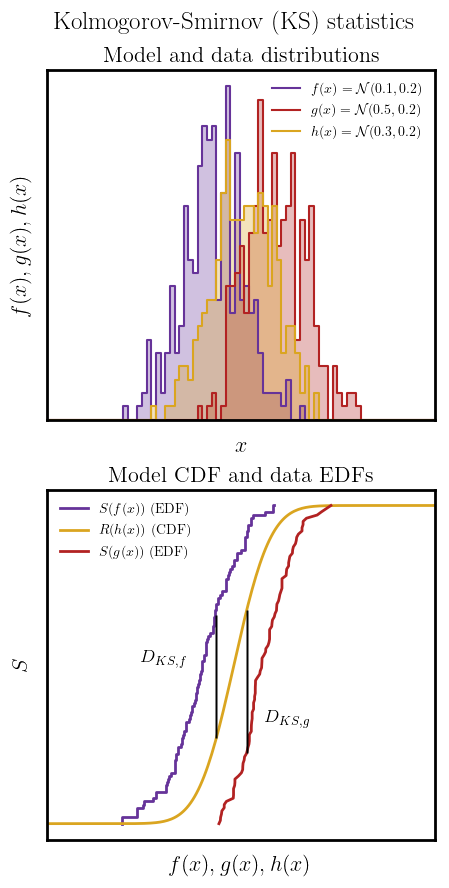
\includegraphics[width=0.8\columnwidth]{figures/graphs/ks_diagram.png}
% \centering
% \caption{An illustration of the KS statistic for two data distributions $f(x)$ and $g(x)$ and one model distribution 
% $h(x)$. The model cumulative distribution function (CDF) and data empricial distribution functions (EDFs) are shown.}
% \label{fig:ks_diagram}
% \end{figure}

% The KS test $p$-value $p_{KS}$ is calculated during GAN training. The $p$-value is defined as the probability of 
% obtaining test results at least as extreme as the results actually observed during the test, assuming that the null 
% hypothesis is correct. This translates to quoting the probability of obtaining the KS test statistic $D_{KS}$ given 
% that the distributions are not correlated. The strength of the KS test is that no underlying population distribution 
% function is asserted before calculating $p_{KS}$. The $p_{KS}$ value is referenced against an $\alpha$-value that 
% thresholds the value to reject the null hypothesis with. For $\alpha=0.01$ and a sample size of 64 for each of the 
% compared ensembles in the training loop determinations of $p_{KS}$, this provides a $p$-value of $0.20$. In this work
% all the KS $p$-values were calculated using the SciPy~\cite{scipy} \texttt{stats.ks\_2samp}~function. 







% % % % %%%%%%%%%%%%%%%%%%%%%%%%%%%%%%%%%%%%%%%%%%%%%%%%%%%%%%%%%%%%%%%%%%%%%%%%%%%%%%%%%%%%%%%%%%%%%
% % % % %           references
% % % % %%%%%%%%%%%%%%%%%%%%%%%%%%%%%%%%%%%%%%%%%%%%%%%%%%%%%%%%%%%%%%%%%%%%%%%%%%%%%%%%%%%%%%%%%%%%%


% % % % % \small
% % % % % \bibliographystyle{bibstyle}
% % % % % \bibliography{refs}

%%%%%%%%%%%%%%%%%%%%%%%%%%%%%%%%%%%%%%%%%%%%%%%%%%%%%%%%%%%%%%%%%%%%%%%%%%%%%%%%%%%%%%%%%%%%%%%%%%%%%%%%%%%%%%%%%%%%%%%%%%%
%%%%%%%%%%%%%%%%%%%%%%%%%%%%%%%%%%%%%%%%%%%%%%%%%%%%%%%%%%%%%%%%%%%%%%%%%%%%%%%%%%%%%%%%%%%%%%%%%%%%%%%%%%%%%%%%%%%%%%%%%%%

\section*{Acknowledgements}

Thank you to Prof. Martin Hendry and Dr. Chris Messenger for their time and guidance. I learnt a lot that I will use in the 
future. I am inspired and I look forward to researching AI in cosmology in the future. Thank you to Michael Williams and 
Jordan `McGAN' McGinn for their insights and discussions. 

\footnotesize

% \section*{Declarations}
\subsection*{Data and code availability}
All code can be found at
\url{https://github.com/JedHmr/universe_gen}.
%\footnote{url date:2020-03-21}. 
Some extra material can be found on
\url{http://www.astro.gla.ac.uk/users/jed/} 
%\footnote{url date:2020-03-21} 


% \subsection*{Acknowledgements} 


\end{document}
